\chapter{Verification and Validation of Hybrid Method}
\label{ch:vavohm}

%The verification and validation of the hybrid method focuses on 4 aspects:
%\begin{itemize}
%\item Lamb-Oseen vortex evolution at $Re=1000$ (section \ref{sec:vvhm-love})
%\item Clercx-Bruneau dipole convection at $Re=625$ (section \ref{sec:vvhm-cbdc})
%\item Clercx-Bruneau dipole collision at $Re=550$ (section \ref{sec:vvhm-cbdcoll})
%\item Stalled elliptical airfoil at $Re=5000$ (section \ref{sec:vvhm-ea})
%\item Multi-body problem at $Re=550$ (section \ref{sec:vvhm-mb})
%\end{itemize}

%We investigated several test-cases: the Lamb-Oseen vortex problem, the Clercx-Bruneau dipole collision by Clercx and Bruneau \cite{Clercx2006a}, the impulsively started cylinder test case, an elliptical airfoil at $Re=5000$ and a multi-body problem.

This chapter focuses on the verification and the validation of the hybrid method. The implementation of the hybrid method was first verified using the analytical solutions of the Lamb-Oseen vortex problem, as the test case helped us quantify any errors in the coupling. The validation of the hybrid solver was performed using the test cases provided from literature. The Clercx-Bruneau dipole collision problem of Clercx and Bruneau \cite{Clercx2006a}, provide a detailed analysis on the evolution of the vorticity field and the generation of vorticity from the wall boundary. The impulsively started cylinder problem investigated by Koumoutsakos and Leonard \cite{Koumoutsakos1995a}, and Rosenfeld et al. \cite{MosheRosenFeldDochanKwak1991} showed the evolution of the forces acting on an immersed cylinder in a free-stream flow.

The final stage of the validation was to show the feasibility of simulation the flow around a full VAWT. To perform this we investigated the flow past a stalled airfoil at $Re=5000$, and the flow around a multi-body problem with two cylinders.

\section{Lamb-Oseen Vortex Evolution}
\label{sec:vvhm-love}
The Lamb-Oseen vortex test case simulates the evolution of a laminar vortex core in an unbounded domain. In section \ref{subsec:lagrangianLambOseen}, we used this test case to verify and validate the implementation of the vortex blobs of the Lagrangian solver and in section \ref{subsec:eulerianLambOseen}, we used it to verify the implementation of the Eulerian solver. Therefore, in a similar fashion we employed this test case to verify the coupling of the hybrid solver. 

The unbounded nature of the problem helps us to neglect the influence of the vortex panel on the coupling strategy, and helps us focus on the vorticity field interpolation error discussed in section \ref{subsec:coupling-vpri}. Furthermore, with the analytical solution, we were able to quantitatively present the importance of ensuring conservation of circulation. 

%of wall solid boundary (i.e the wall). Therefore, this test case did not require the panel solver in the Lagrangian solver as we are only concerned with the coupling of the vortex blobs to the Eulerian solver. Thus, we primarily focused on the vorticity field interpolation error discussed in section \ref{subsec:coupling-vpri}. Furthermore, with the analytical solution, we were able to quantitatively present the importance of ensuring conservation of circulation.

%A parameter sensitivity analysis was therefore performed to determine their effects on the coupling error.
Moreover, we were able to quantify the influences of the discretization on the accuracy of the coupling. The parameters that determine the spatial discretization of the vortex blobs are the nominal particle spacing $h$, and the overlap ratio $\lambda$ (see Figure \ref{fig:blobOverlap}). The spatial discretization of the Eulerian solver is regarded as a control variable for this test case as its impact was concluded in section \ref{subsec:eulerianLambOseen}. The parameters that determine the temporal discretization of the hybrid method are the time step size of the Eulerian solver $\Delta t_E$, and the time step size of the Lagrangian solver $\Delta t_L$. These are determined according to equation \ref{eq:timeStepDependency}, with $k_E$ being the number of Eulerian sub-steps.

%The coupling error was quantified by determining the growth of maximum relative error in vorticity $\epsilon_{\omega}$ given by equation \ref{eq:maxRelErrorDef}, the approach used in section \ref{subsec:lagrangianLambOseen} and in section \ref{subsec:eulerianLambOseen}. 


\subsection{Problem Definition}

The Lamb-Oseen Vortex problem is defined by the vorticity field and the velocity field, equations \ref{eq:lo_voeq} and \ref{eq:lo_veeq}, respectively. The hybrid solver is initialized by first assigning the strengths of the vortex blobs using equation \ref{eq:lo_pie}. The Eulerian domain $\Omega_E$ is then initialized using the solution of the Lagrangian solver. Daeninck \cite{Daeninck2006} used this approach to enhance the coupling between the methods ensuring minimum interpolation error.

Figure \ref{fig:HLO_dc} shows the hybrid domain configuration for the Lamb-Oseen vortex problem with the Lagrangian domain $\Omega_L$ spanning the full fluid domain. The Eulerian domain $\Omega_E$ only resolves the center of the Lamb-Oseen core, $\Omega_E = [-0.5,-0.5] \times [-0.5,-0.5]$. The boundary of the Eulerian domain $\partial \Omega_E$ is a Dirichlet velocity boundary $\partial \Omega_E = \Sigma_d$ where the velocity boundary condition is applied, as described in section \ref{subsec:hybrid-ca}. The correction of the Lagrangian domain is performed in the interpolation domain $\Omega_{I}$ according to the procedures described in section \ref{sec:coupling-mlca}. The outer boundary of the interpolation domain $\Sigma_{o}$ is defined with an offset $d_{bdry}$ from the Eulerian boundary $\Sigma_d$ by a distance $d_{bdry} = 2\cdot h$, where $h$ is the nominal blob spacing. Similar choice was made by Stock \cite{Stock2010a} (discussed in section \ref{subsec:hybrid-lcs}), and ensures that the potential inaccuracies at the outer Eulerian boundary is ignored during the interpolation procedure.

	\begin{figure}[!b]
	\centering
	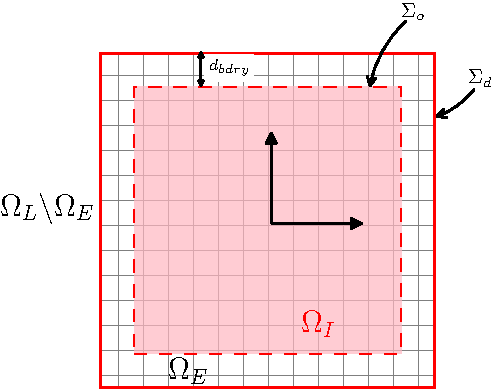
\includegraphics[width=0.5\linewidth]{./figures/validation/lambOseen/hlo_dd-crop.pdf}
	\caption{(\textit{Not to scale}) The domain decomposition for the Lamb-Oseen vortex problem, $\Omega_E$. The Eulerian domain is defined as $\Omega_E = [-0.5,0.5]\times[-0.5,0.5]$ with Dirichlet boundary $\Sigma_d$ [{\color{plotRed}{---}}, solid red]. The parameters of the discretization are tabulated in table \ref{tab:HLO_pt}.}
	\label{fig:HLO_dc}
	\end{figure}

The spatial discretization of the Eulerian domain $\Omega_E$ is regarded as a control (i.e fixed) variable. Therefore, the parameter sensitivity analysis is performed by varying the discretization of the Lagrangian method only. The Eulerian domain is discretized with an unstructured mesh generated with GMSH (see section \ref{subsec:mgugmsh}) having, $N_{cells} = 26448$  and grid size $h_{grid}$ ranging from $0.007$ to $0.0016$. 

The Lamb-Oseen vortex problem is defined according to the parameters tabulated in table \ref{tab:HLO_pt}. The center of the core is located at $(x,y)=(0,0)$, where the Eulerian domain $\Omega_E$ is also centered. The parameters are chosen such that vorticity $\omega$ and velocity $\mathbf{u}$ is non-zero at the boundary of the Eulerian domain $\Sigma_d$, Figure \ref{fig:HLO_dc}. The evolution of the Lagrangian solver and the Eulerian solver is performed according to sections \label{sec:eu-eotlm} and \ref{sec:eu-eotem} respectively.

% The Lagrangian solver performs TRS for diffusion of the vortex blobs, see section \ref{subsubsec:srs}. The scheme requires vortex blob redistribution at every step, $f_{redis} = 1$. In conjunction with the redistribution, the population control is also performed at every step, $f_{pc}=1$ with $(\Gamma_{loc},\Gamma_{glob})$ as tabulated in table \ref{tab:HLO_pt}.

\subsection{Results and Discussion}

The investigation of the Lamb-Oseen vortex problem is divided into three parts. The first part of the investigation concerns with comparing several stages of the hybrid coupling, defined in section \ref{subsec:UvOvF}. We compared the uncoupled scheme with the one-way coupled scheme and with the fully coupled scheme. These successive coupling investigation helped us determine the source of the error, and furthermore quantify the errors in the coupling process. The second part of the investigation, section \ref{subsubsec:coc} focuses on importance of conservation of circulation that was discussed in section \ref{subsec:coupling-cotc}. The results of the non-conserved and conserved scheme are compared to conclude the importance of conservation of circulation. During these two investigations, the parameters tabulated in table \ref{tab:HLO_pt} are used. The third and final investigation is dedicated to the parameter sensitivity analysis, section \ref{subsubsec:psa}. The parameters that determine the spatial and temporal discretization of the scheme is investigated to verify the convergence of scheme.

	\ctable[
		caption = {Summary of the parameters for the Lamb-Oseen vortex evolution.},
		label   = {tab:HLO_pt},
		pos = !t,]{lcll}{}{\FL
		
		Parameters 					& Value 	& Unit					& Description \ML
		$\Gamma_c$\T               	& 1 &\si{m^2.s^{-1}} 				& Core strength\\
		$\Omega$               		& $[-0.5,0.5]\times[-0.5,0.5]$ &\si{m}		& Eulerian domain bounds \\
		$\nu$						& $0.001$ &\si{kg.s^{-1}.m^{-1}}& Kinematic viscosity\\
		$ \tau$ 		    		& $100$ 	&\si{s}	& Lamb-Oseen time constant\\
		$\lambda$						& 1 & - & Overlap ratio\\
		$h$							& 0.01 & \si{m} & Nominal blob spacing\\
		$(\Gamma_{loc},\Gamma_{glob})$			& (\num{1e-14}, \num{1e-14}) & - & Population control threshold\\
		$h_{grid}$ 					& \numrange{0.007}{0.016} & \si{m} & FE cell diameter span \\
		$ N_{\mathrm{cells}}$ 		& $26448$ 	& -						& Number of mesh cells\\
		$\Delta t_L$				& 0.001 & \si{s} & Lagrangian time step size\\
		$\Delta t_E$				& 0.001 & \si{s} & Eulerian time step size\\		
		$k_E$						& 1 & - & Eulerian sub-steps\\
		$ N_{\mathrm{t-steps}}$ 	& 1000 & -				& Number of time integration steps\\
		$t$ 		    			& \numrange{0}{1} 	&\si{s}			& Simulation time span\\		
		$d_{bdry}$					& $2\cdot{h}$ & \si{m} & Interpolation boundary offset from $\Sigma_o$\LL}

\subsubsection{Uncoupled vs. One-way Coupled vs. Fully Coupled}
\label{subsec:UvOvF}
The several stages of the hybrid coupling with the fully Eulerian test case, to verify the implementation of the hybrid algorithm. The three stages of the coupling are as follows:

\begin{itemize}
\item \textbf{Uncoupled}: In the uncoupled test case, we only focus on the Eulerian subdomain of the hybrid scheme, Figure \ref{fig:HLO_dc}. The boundary conditions for the Eulerian Dirichlet boundary are obtained directly from the analytical solution, equation \ref{eq:eLO_veq}. This test helps us quantify the base error due the nature of the FEM serves as the benchmark for further investigation.
\item \textbf{One-way coupled}: The one-way coupled test case is a partially coupled hybrid scheme. Here the Eulerian method obtains the boundary condition from the Lagrangian method and the Lagrangian subdomain remains unmodified throughout the simulation. The purpose of this test cases is to quantify any error due the transfer of the solution from Lagrangian to Eulerian method.
\item \textbf{Fully coupled}: The fully coupled test case performs the full coupling strategy, according to the steps described in section \ref{subsec:hybrid-ca}. The Eulerian method is evolved using the Lagrangian solution. At the end of each time step, the Lagrangian solution inside the interpolation domain $\Omega_{I}$, Figure \ref{fig:HLO_dc}, is corrected. This test case helped us quantify the error in transferring the Eulerian solution to the Lagrangian method.
\end{itemize}
	
	\begin{figure}[!b]
     \centering
     \begin{subfigure}[t]{0.45\textwidth}
             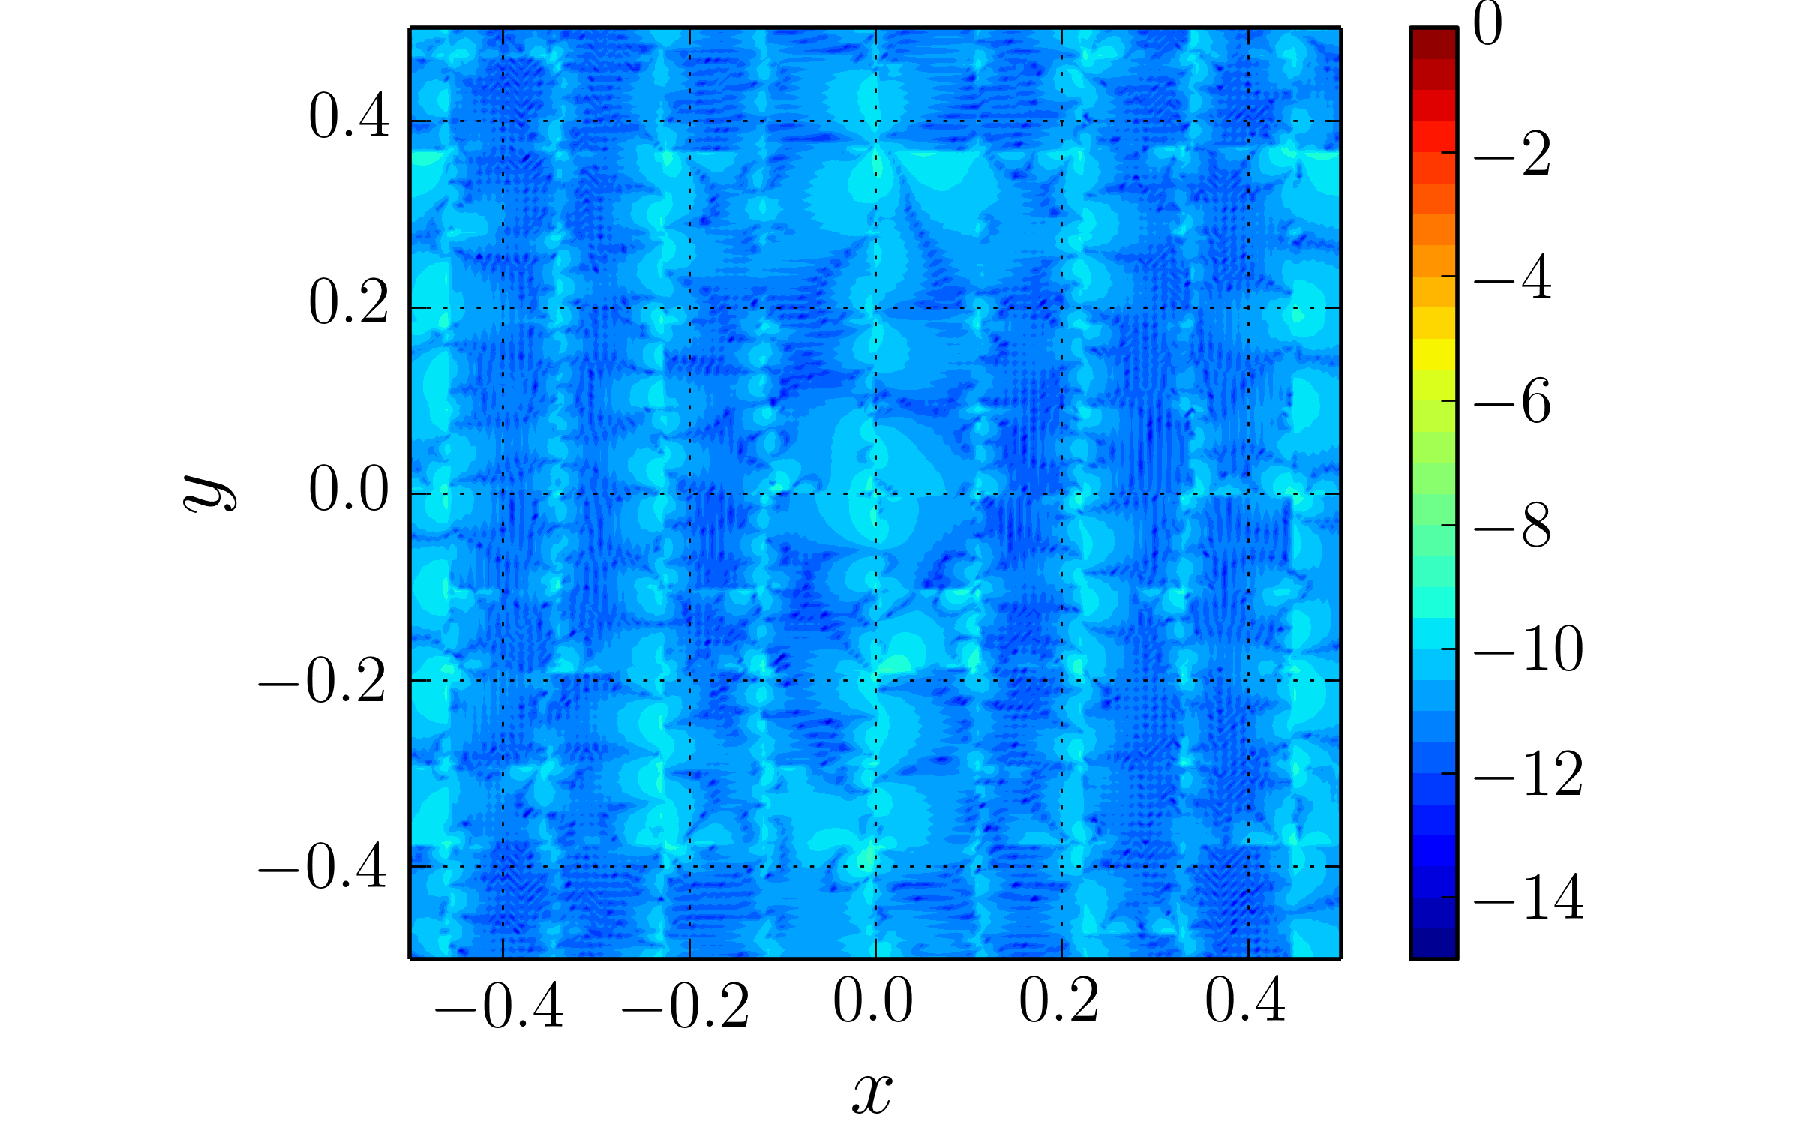
\includegraphics[width=\linewidth]{./figures/validation/lambOseen/lambOseen_fully_vErrorInitial_raster.png}
             \caption{Velocity}
             \label{fig:lambOseen_oneway_vErrorInitial}
     \end{subfigure}%
     \qquad %add desired spacing between images, e. g. ~, \quad, \qquad etc.
       %(or a blank line to force the subfigure onto a new line)
     \begin{subfigure}[t]{0.45\textwidth}
             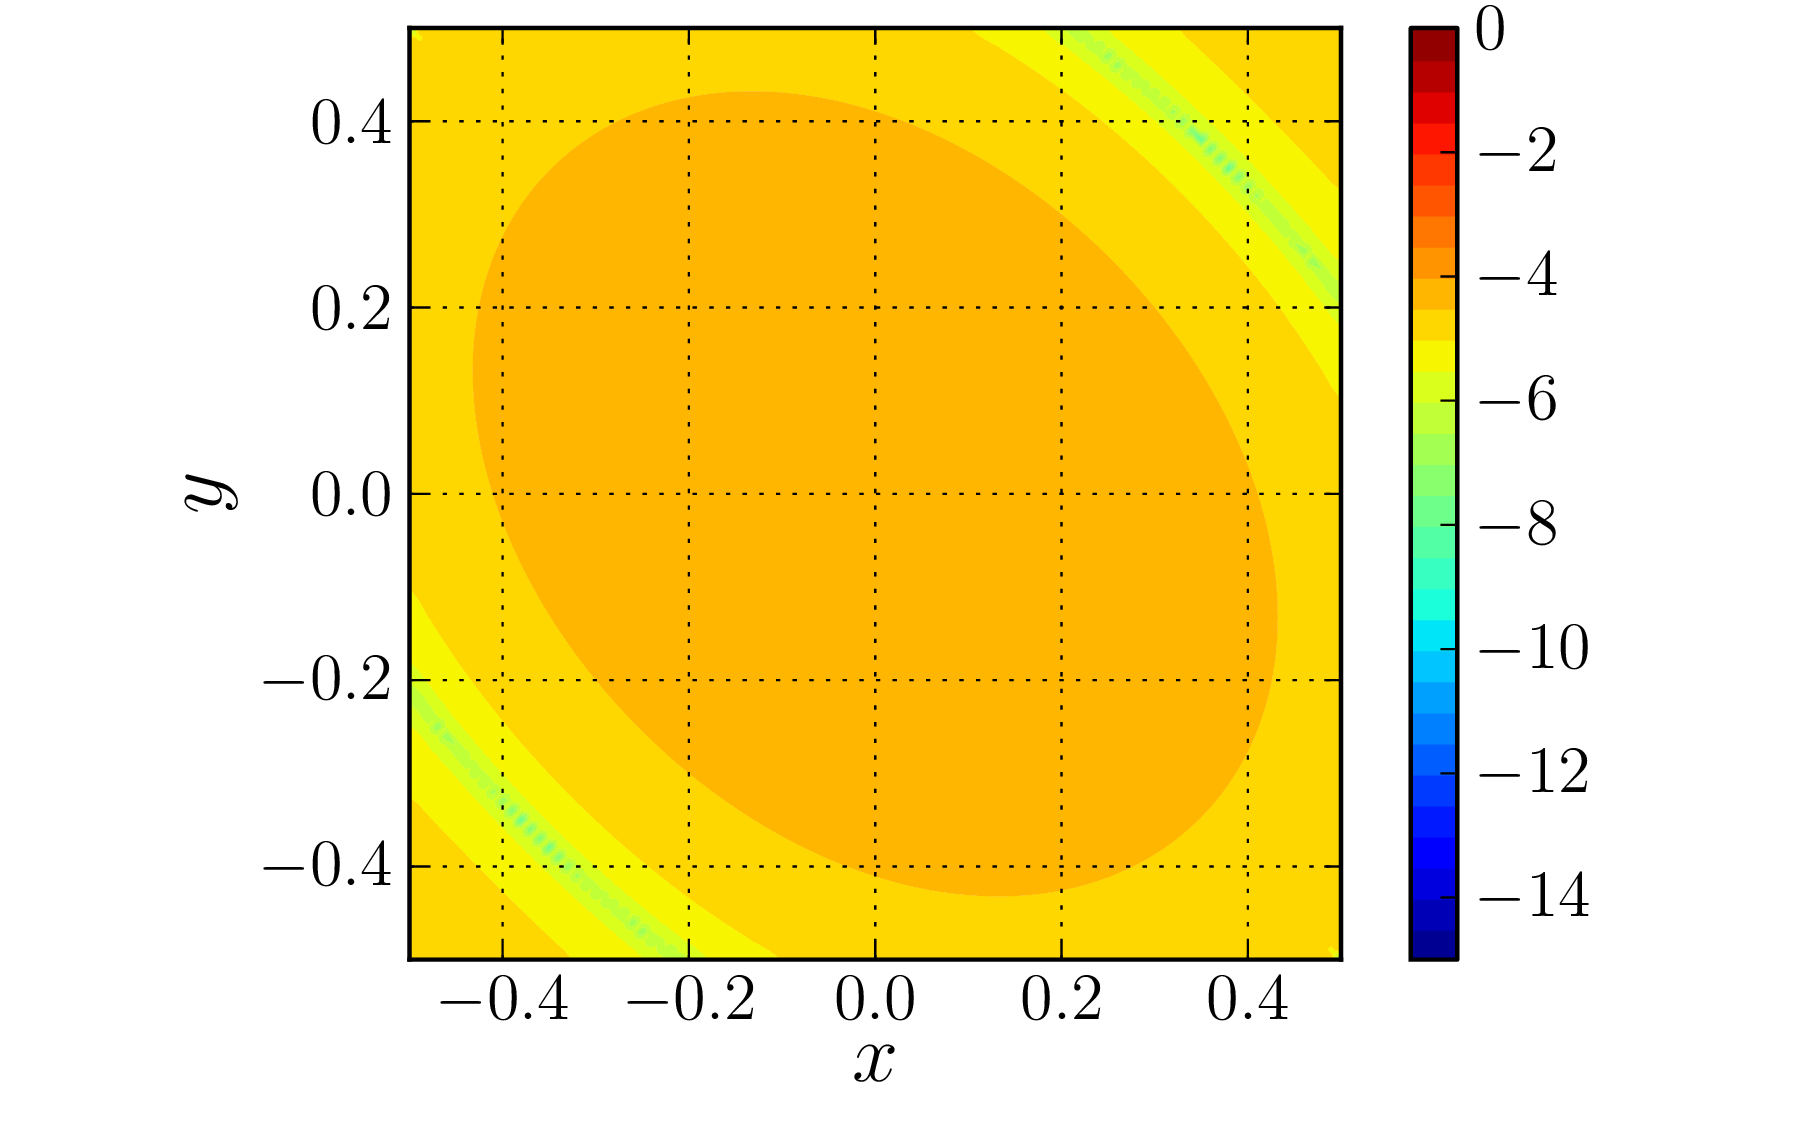
\includegraphics[width=\linewidth]{./figures/validation/lambOseen/lambOseen_fully_wErrorInitial_compressed.png}
             \caption{Vorticity}
             \label{fig:lambOseen_uncoupled_wErrorInitial}
     \end{subfigure}
     \caption{Initial relative error at $t=0$ inside the Eulerian domain $\Omega_E$. The figure depicts \textbf{(a)} the relative error in velocity $\mathbf{u}$, and \textbf{(b)} the relative error in vorticity $\omega$.}
     \label{fig:lambOseen_initialError}
	\end{figure}
		
Figure \ref{fig:lambOseen_initialError} depicts the initial relative error in velocity and vorticity inside the Eulerian domain $\Omega_E$. The relative error in velocity is near machine epsilon $\epsilon \le \num{e-10}$, but the error in vorticity is in the order of \num{e-5}. This occurs because the solution was initialized using the velocity field and the vorticity was determined numerically as described in section \ref{subsec:dtvf}. Therefore, the increase in the error shown in figure is as expected.

	\begin{figure}[!t]
	\centering
	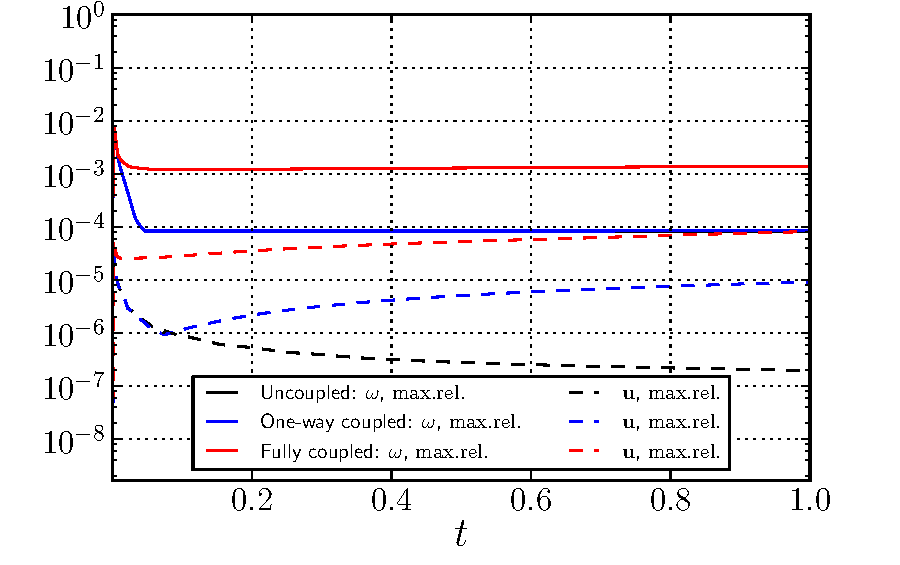
\includegraphics[width=0.6\linewidth]{./figures/validation/lambOseent2/lambOseen_comparision_corrected.pdf}
	\caption{Evolution of the maximum relative error in velocity (dashed) and the maximum relative error in vorticity (solid), equation \ref{eq:maxRelErrorDef}, from $t=0$ to $t=1$, using the parameters tabulated in table \ref{tab:HLO_pt}. The figure compares uncoupled case (\textbf{black}) vs. the one-way coupled case ({\color{plotBlue}{\textbf{blue}}}) vs. the fully coupled case ({\color{plotRed}{\textbf{red}}}).}
	\label{fig:lambOseen_comparison}
	\end{figure}

Figure \ref{fig:lambOseen_comparison} shows the evolution of maximum relative error in vorticity $\omega$ and velocity $\mathbf{u}$ of the uncoupled, one-way coupled and the fully coupled cases inside the Eulerian domain $\Omega_E$ w.r.t. the analytical solution, equation \ref{eq:lo_voeq}. The initial observation shows that the error in velocity is two to three orders of magnitude lower than the error in vorticity. The figure shows that the uncoupled scheme has the lowest error in vorticity and velocity. This is expected as the boundary condition is directly obtained from the analytical solution and therefore minimum error is introduced. As time progresses, the error in velocity converges near \num{e-7} and the error in vorticity converges near \num{e-4}.

	\begin{figure}[!b]
     \centering
     \begin{subfigure}[t]{0.45\textwidth}
             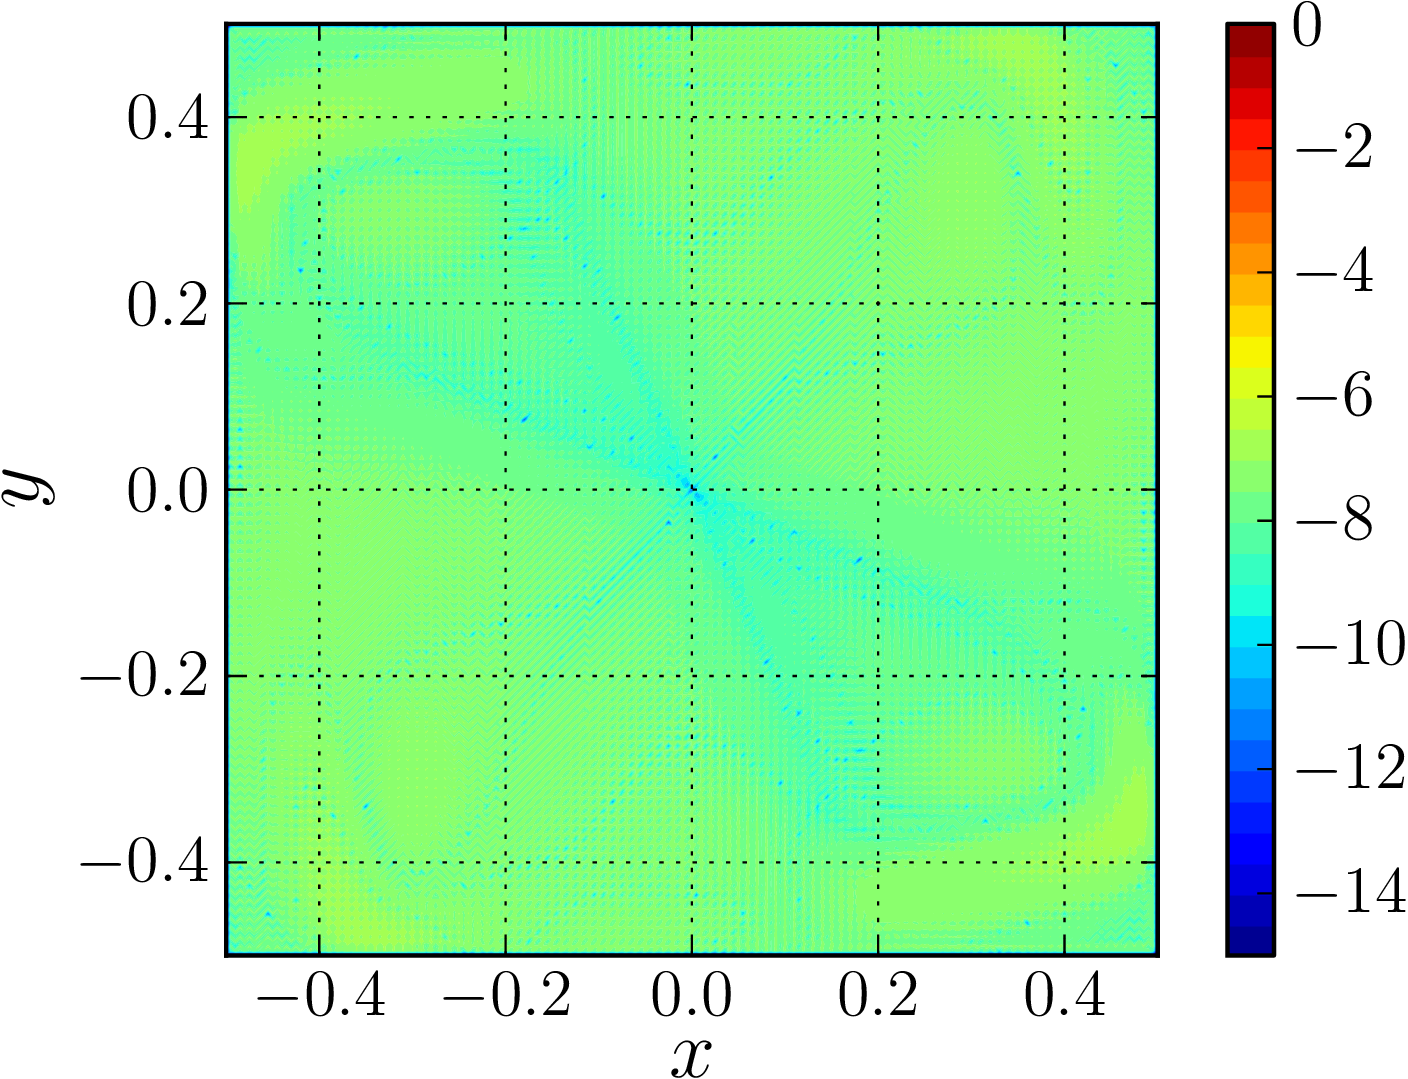
\includegraphics[width=\linewidth]{./figures/validation/lambOseent2/lambOseen_uncoupled_vErrorFinal_compressed-crop.png}
             \caption{Uncoupled; velocity $\mathbf{u}$}
             \label{fig:lambOseen_uncoupled_vErrorFinal}
     \end{subfigure}%
     \qquad %add desired spacing between images, e. g. ~, \quad, \qquad etc.
       %(or a blank line to force the subfigure onto a new line)
     \begin{subfigure}[t]{0.45\textwidth}
             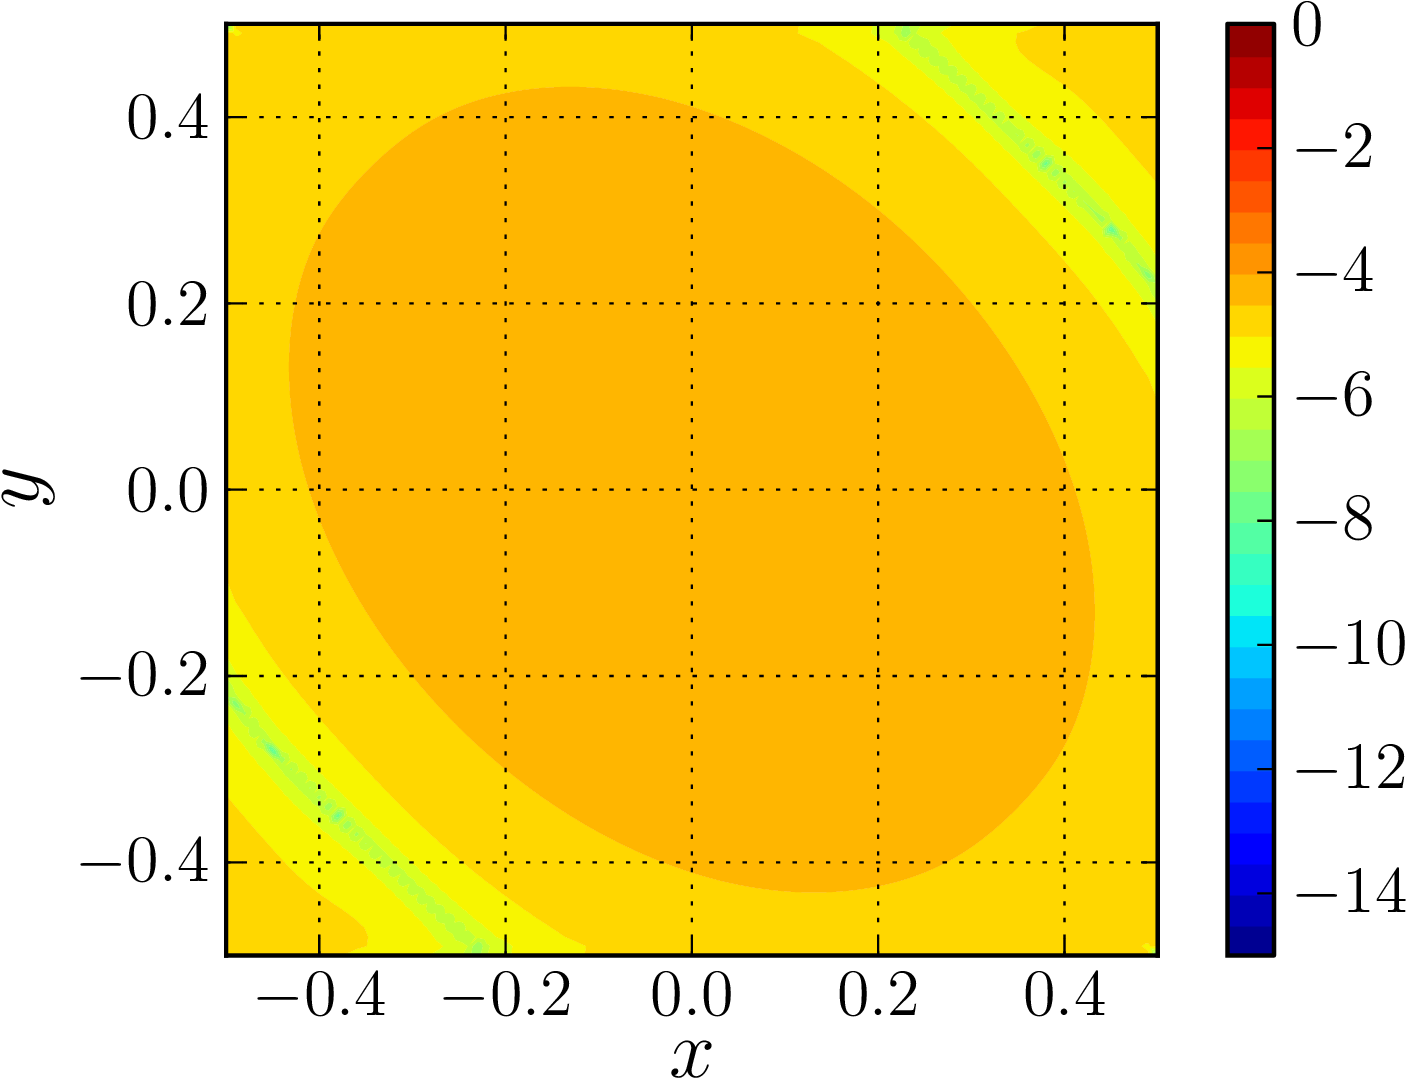
\includegraphics[width=\linewidth]{./figures/validation/lambOseent2/lambOseen_uncoupled_wErrorFinal_compressed-crop.png}
             \caption{Uncoupled; vorticity $\omega$}
             \label{fig:lambOseen_uncoupled_wErrorFinal}
     \end{subfigure}%       
       
     \begin{subfigure}[t]{0.45\textwidth}
             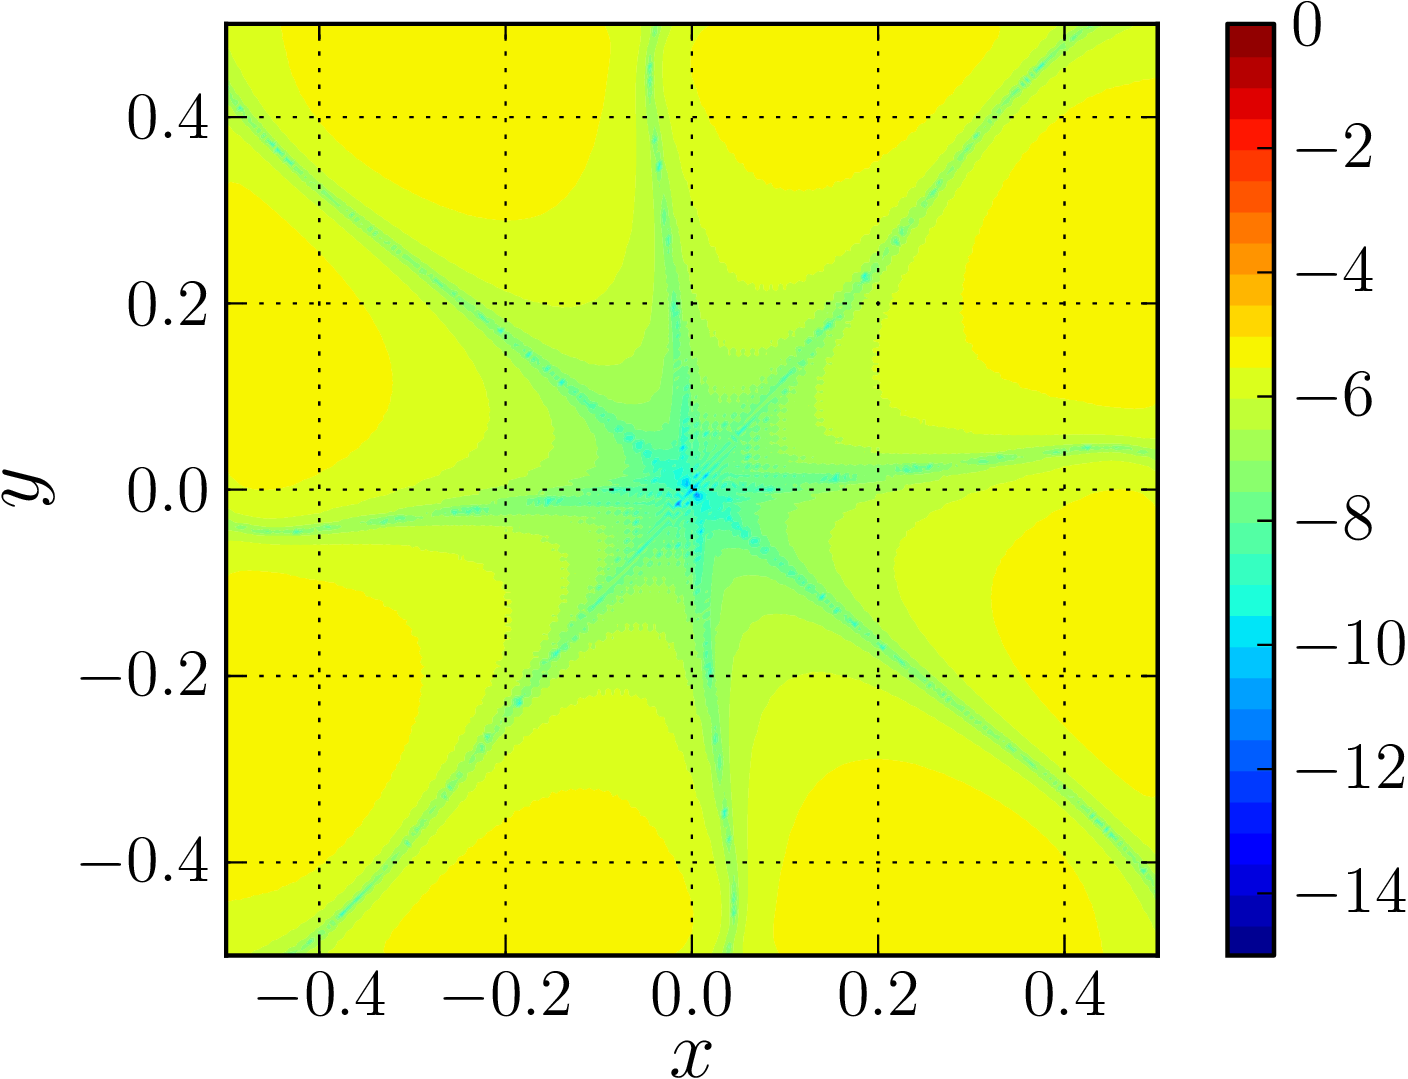
\includegraphics[width=\linewidth]{./figures/validation/lambOseent2/lambOseen_oneway_vErrorFinal_compressed-crop.png}
             \caption{One-way coupled; velocity $\mathbf{u}$}
             \label{fig:lambOseen_oneway_vErrorFinal}
     \end{subfigure}
     \qquad
     \begin{subfigure}[t]{0.45\textwidth}
             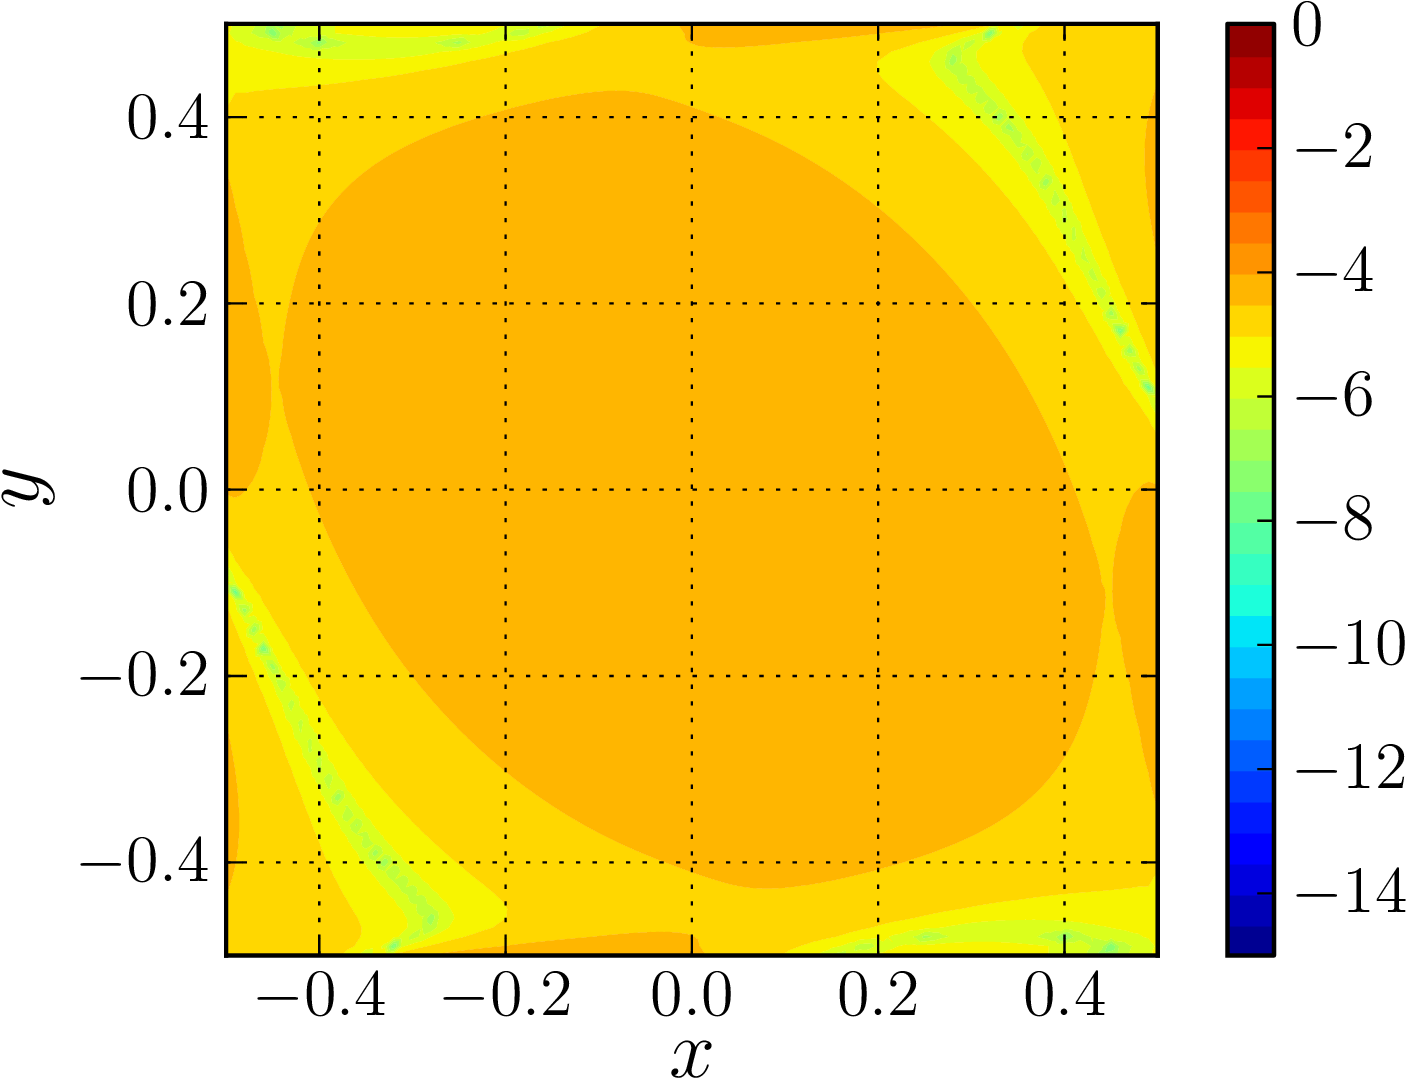
\includegraphics[width=\linewidth]{./figures/validation/lambOseent2/lambOseen_oneway_wErrorFinal_compressed-crop.png}
             \caption{One-way coupled; vorticity $\omega$}
             \label{fig:lambOseen_oneway_wErrorFinal}
     \end{subfigure}     
   
     \begin{subfigure}[t]{0.45\textwidth}
             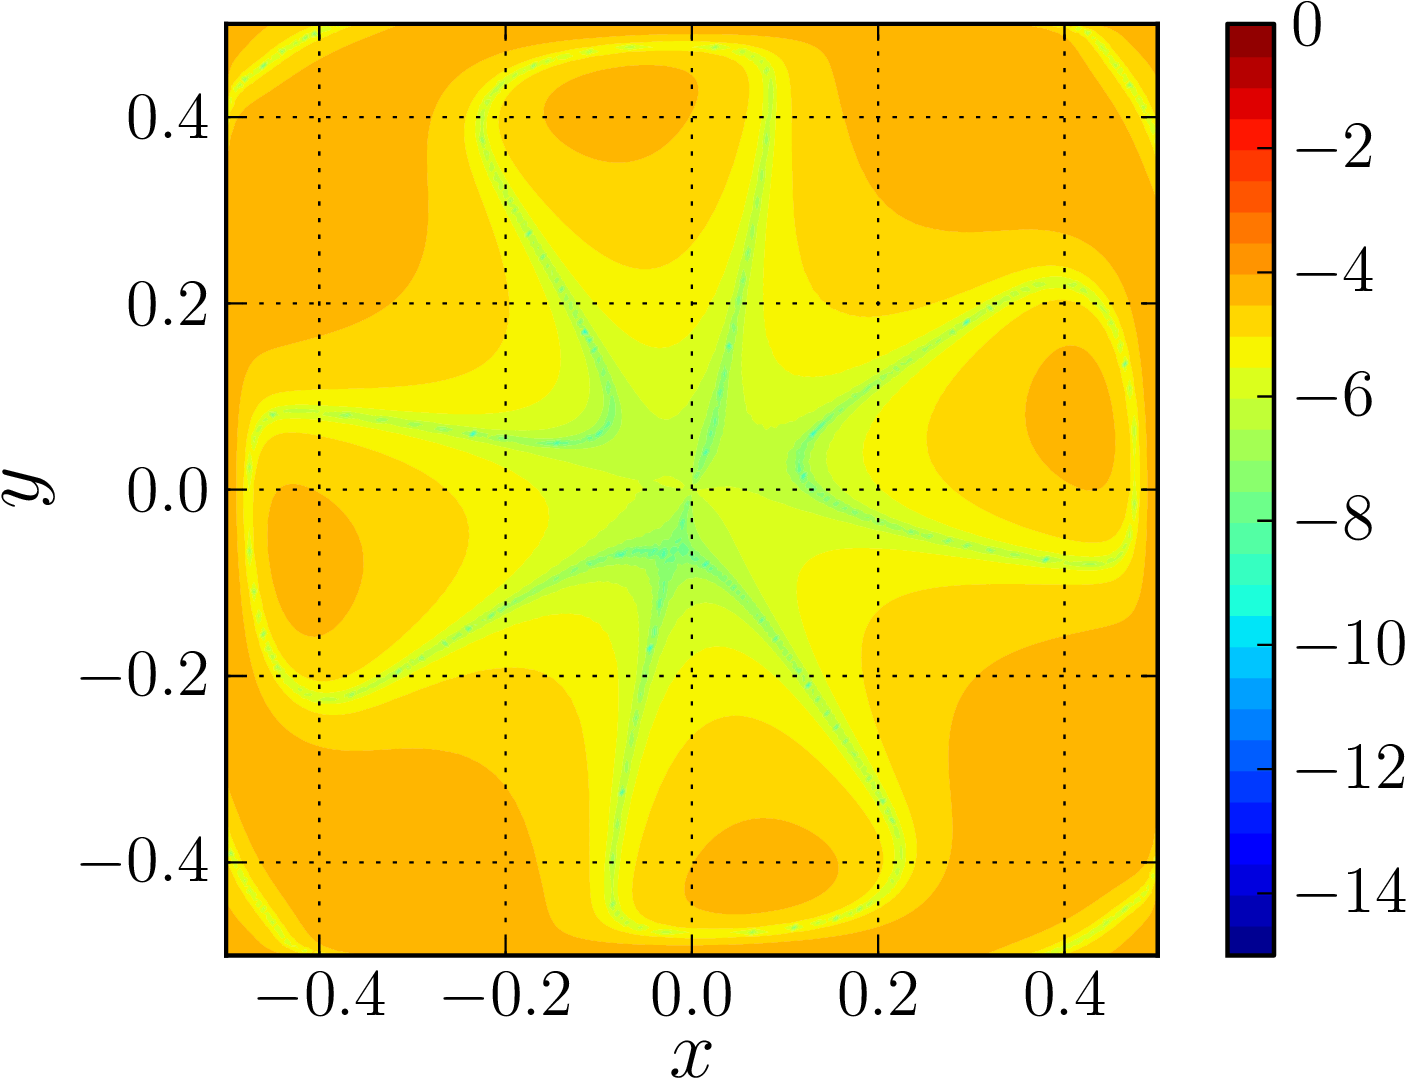
\includegraphics[width=\linewidth]{./figures/validation/lambOseent2/lambOseen_fully_vErrorFinal_compressed-crop.png}
             \caption{Fully coupled; velocity $\mathbf{u}$}
             \label{fig:lambOseen_fully_vErrorFinal}
     \end{subfigure}     
     \qquad
     \begin{subfigure}[t]{0.45\textwidth}
             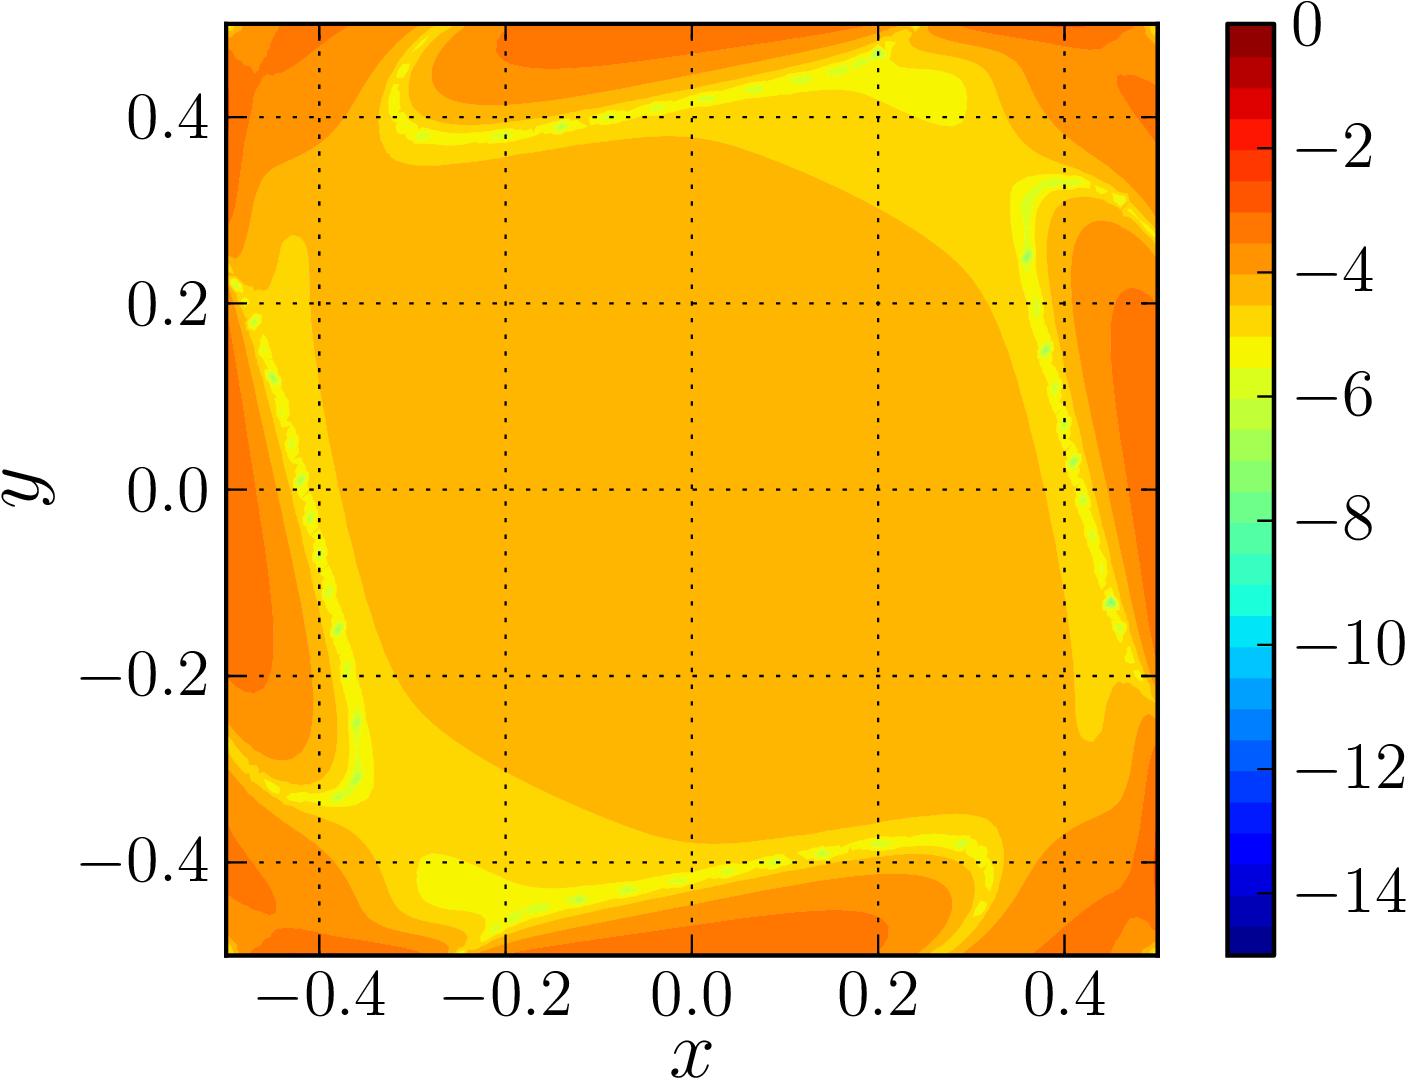
\includegraphics[width=\linewidth]{./figures/validation/lambOseent2/lambOseen_fully_wErrorFinal_compressed-crop.png}
             \caption{Fully coupled; vorticity $\omega$}
             \label{fig:lambOseen_fully_wErrorFinal}
     \end{subfigure}        
     
     \caption{Plot of the relative error in velocity (\textit{left}) and relative error in vorticity (\textit{right}) in the Eulerian domain $\Omega_E$ at $t=1$. The figure compares the error between \textbf{(a)}\textbf{(b)} the uncoupled, \textbf{(c)}\textbf{(d)} the one-way coupled, and \textbf{(e)}\textbf{(f)} the fully coupled cases.}
     \label{fig:lambOseen_finalError}
	\end{figure}

The one-way coupled case shows an increase in the relative error in velocity field $\mathbf{u}$ inside the Eulerian domain $\Omega_E$. However, the difference is negligible at the initial stages of the simulation. This states that the analytical solution was well represented by the vortex blobs with a small discretization error. At $t=1$, the error in velocity increases by two orders of magnitude from \num{e-7} to \num{e-5}, w.r.t to the uncoupled scheme. This was expected as the velocity boundary conditions for the Eulerian domain is obtained from the discrete solution of the Lagrangian method. In section \ref{subsec:lagrangianLambOseen}, we observed the behavior of evolution of the Lagrangian solution and this behavior is introduced into the Eulerian method. To investigate the convergence of this error, we will later investigated the error for various Lagrangian discretizations.

The fully coupled case demonstrates that there is an additional source of error. Unlike the one-way coupled case, the increase in the error is observed from the start of the simulation, implying that this is due to the correction of the strengths of the vortex blobs. In section \ref{subsec:coupling-vpri}, we discussed that the re-initialization of the vortex blobs introduces smoothing error in the vorticity field (i.e the Gaussian blurring of the vorticity field). This causes the Lagrangian solution to further deviate from the analytical solution of the Lamb-Oseen vortex. The consequence of this was that at $t=1$, the error in vorticity $\epsilon_{\omega}$ increased from \num{e-4} to \num{e-3} and the error in velocity increased from \num{e-5} to \num{e-4}, w.r.t the one-way coupled case.

%The transfer of the discrete vorticity field from the Eulerian method to the Lagrangian method (i.e the correction process) causes an additional increase in the discretization error of the Lagrangian solution. This causes the Lagrangian solution to further deviate from the analytical solution of the Lamb-Oseen vortex. The main component of the discretization error is the smoothing error (i.e Gaussian blurring of the vorticity field) when using mollified vortex kernels, discussed in section \ref{subsec:hy_iwtca}. The Gaussian blurring of the vorticity field adds an additional error when re-initializing the vortex blobs inside the interpolation domain $\Omega_{int}$.		

Figure \ref{fig:lambOseen_finalError} shows the relative error in velocity and vorticity inside the Eulerian domain $\Omega_E$ at $t=1$, for the three stages of coupling. We observe that there is an increase in error when going from the uncoupled scheme to the one-way coupled scheme to the fully coupled. Comparing the uncoupled scheme to the one-way coupled scheme, an increase in error is observed at the boundary of the Eulerian domain $\Sigma_d$.  Comparing the one-way coupled to fully coupled case, we see that there is an additional increase in the error from the boundary. Therefore, the artificial vorticity generated from the boundary is due to the mismatch in the solutions of the Eulerian and the Lagrangian method. A larger mismatch in the solution will introduce strong artificial vorticity at the boundary.
%The error originates from the small error in the Dirichlet boundary conditions at the boundary $\Sigma_d$. due to the larger error in the Dirichlet boundary condition. Figure \ref{fig:lambOseen_fully_wErrorFinal} clearly shows this artificial vorticity generated from the boundary, and can be concluded that this is due to the mismatch in the solutions of the Eulerian and the Lagrangian method.

Thus, we were able to determine the sources of the errors in the hybrid coupling. The error in vorticity, represented by the artificial vorticity near the outer Eulerian boundary $\Sigma_o$, is a culmination of the discretization error of the Lagrangian method and the Eulerian method. Therefore, if we were to use a higher resolution, we expect a greater matching of the Eulerian method and the Lagrangian method. Section \ref{subsubsec:psa}, is dedicated to validate this claim.


%The error in vorticity ()we observe here vorticity is culmination of errors introduced during various stages of coupling. %The strength of the artificial vorticity at the boundary is proportional to the error in the coupling and to ensure an accurate coupling scheme, we have ensure this vorticity does not corrupt the characteristics of the original vorticity field. Therefore, we modified the discretization of the Lagrangian field such that the artificial vorticity generated from the boundary is less the threshold of influence (i.e $<1\%$ of the maximum vorticity $\max\{\omega\}$).

\subsubsection{Conservation of circulation}
\label{subsubsec:coc}

The approach for ensuring conservation of circulation during the coupling process was discussed in section 	\ref{subsec:coupling-cotc}. To validate the importance of conservation of circulation, we ran two simulations with and without the conservation of circulation during the transfer of vorticity from the Eulerian method to the Lagrangian method. The control variables of the simulation are the parameters tabulated in table \ref{tab:HLO_pt}.

	\begin{figure}[!b]
     \centering
     \begin{subfigure}[t]{0.45\textwidth}
             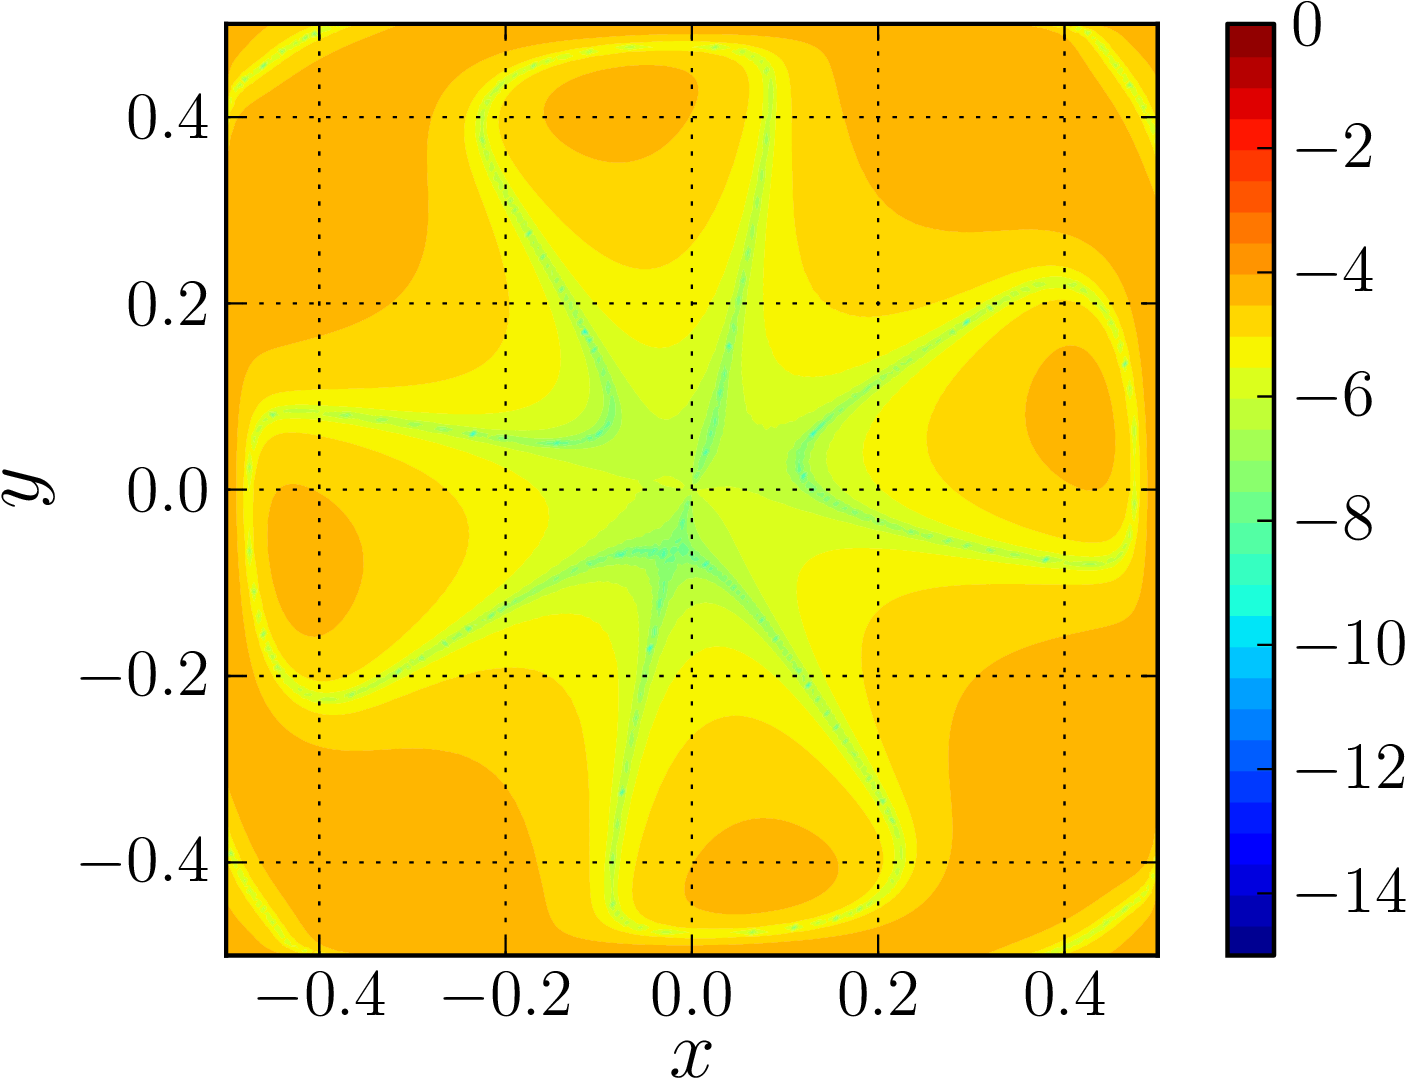
\includegraphics[width=\linewidth]{./figures/validation/lambOseent2/lambOseen_fully_vErrorFinal_compressed-crop.png}
             \caption{Conservation \texttt{on}; velocity $\mathbf{u}$}
             \label{fig:lambOseen_fullyCon_vErrorFinal}
     \end{subfigure}%
     \qquad %add desired spacing between images, e. g. ~, \quad, \qquad etc.
       %(or a blank line to force the subfigure onto a new line)
    \begin{subfigure}[t]{0.45\textwidth}
             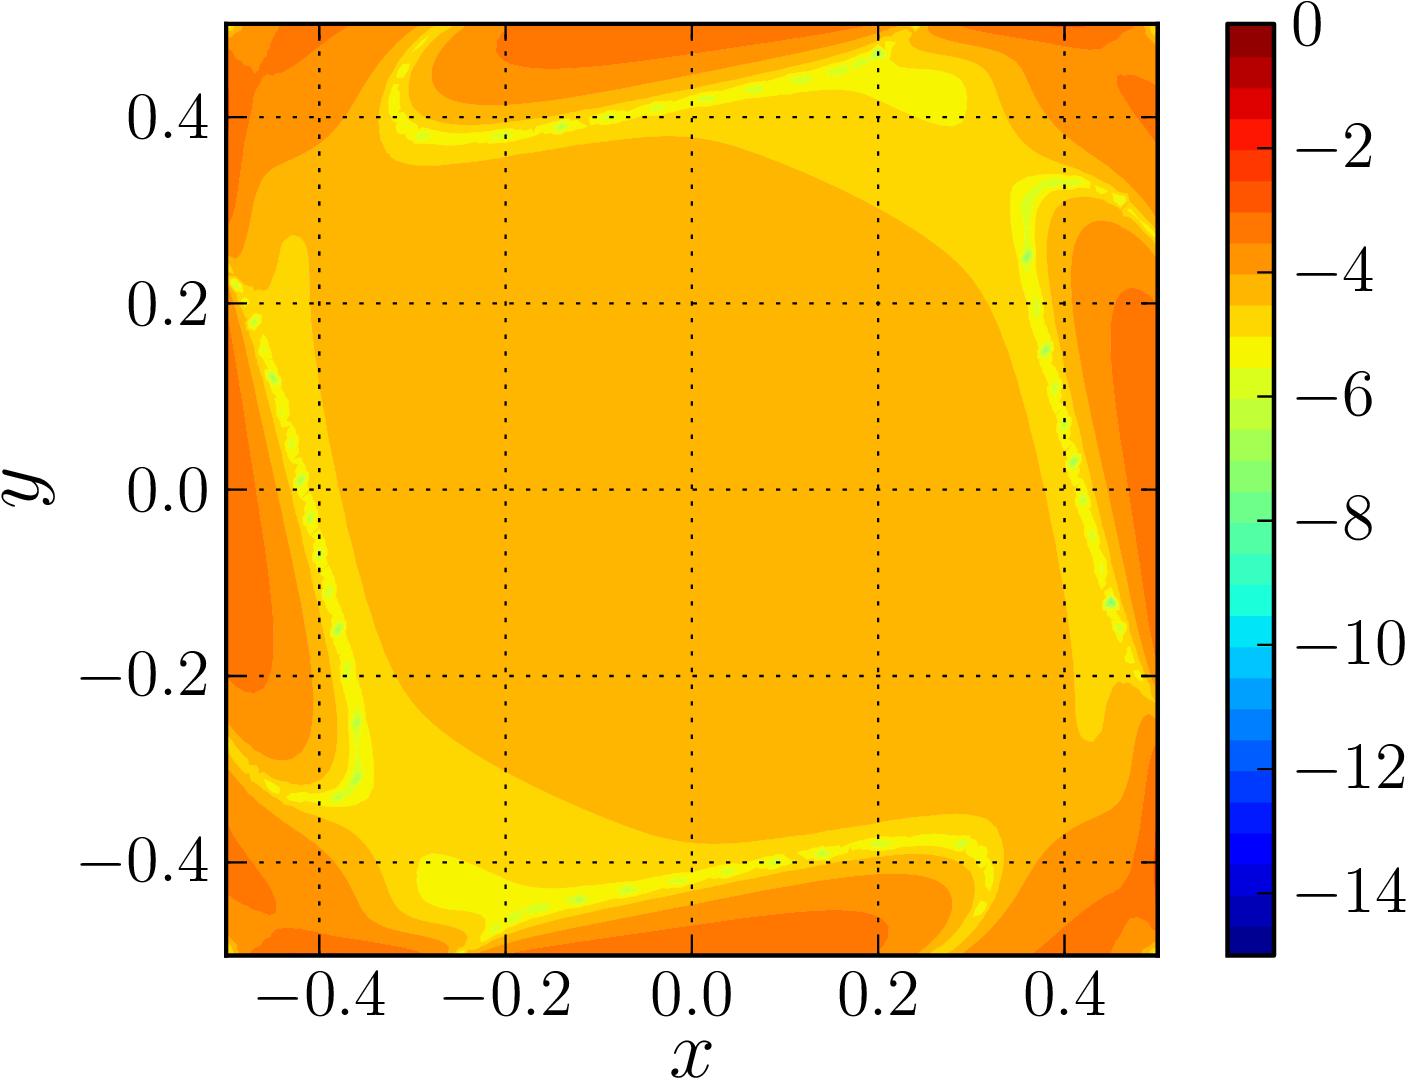
\includegraphics[width=\linewidth]{./figures/validation/lambOseent2/lambOseen_fully_wErrorFinal_compressed-crop.png}
             \caption{Conservation \texttt{on}; vorticity $\omega$}
             \label{fig:lambOseen_fullyCon_wErrorFinal}
     \end{subfigure}%     
            
     \begin{subfigure}[t]{0.45\textwidth}
             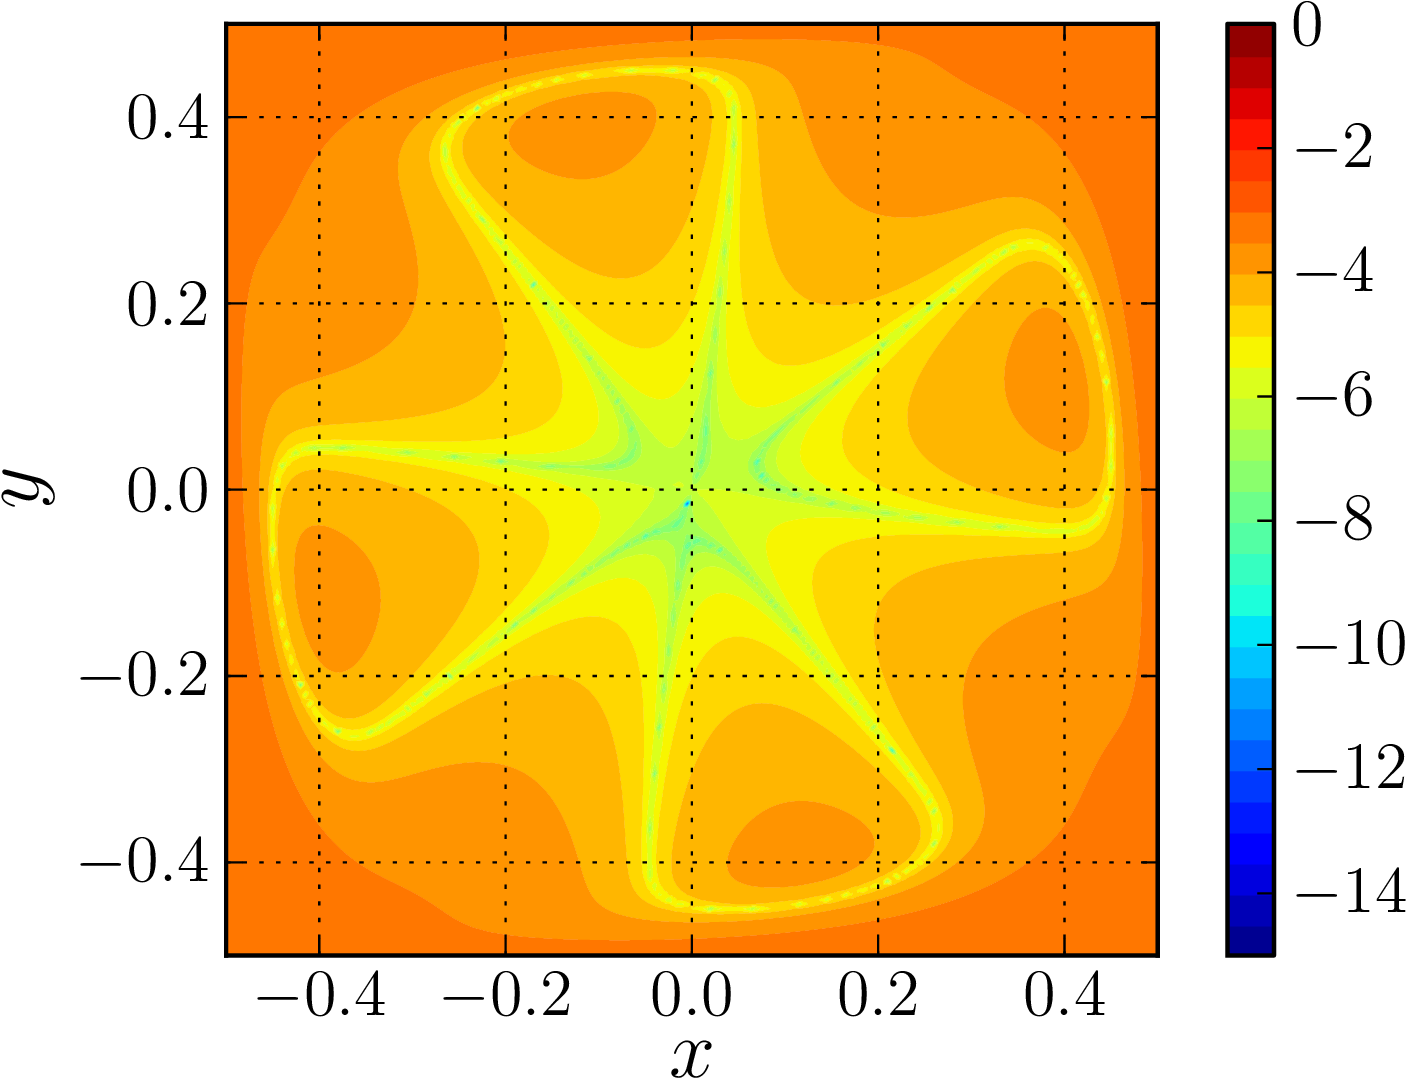
\includegraphics[width=\linewidth]{./figures/validation/lambOseent2/lambOseen_fullyCoff_vErrorFinal_compressed-crop.png}
             \caption{Conservation \texttt{off}; velocity $\mathbf{u}$}
             \label{fig:lambOseen_fullyCoff_vErrorFinal}
     \end{subfigure}
     \qquad     
     \begin{subfigure}[t]{0.45\textwidth}
             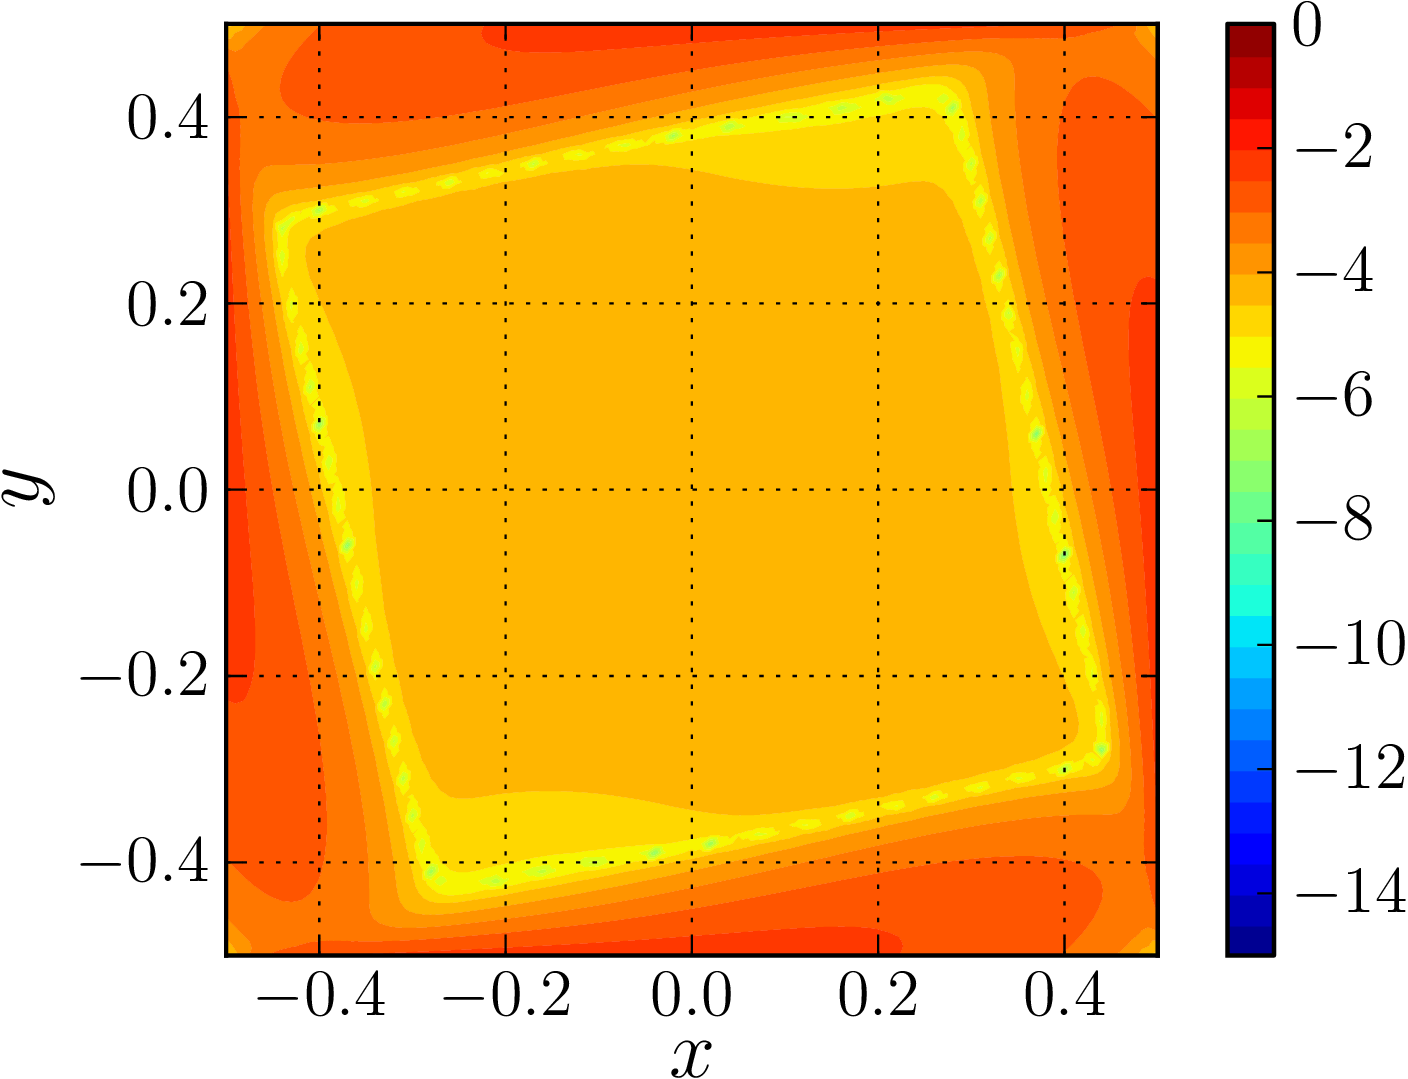
\includegraphics[width=\linewidth]{./figures/validation/lambOseent2/lambOseen_fullyCoff_wErrorFinal_compressed-crop.png}
             \caption{Conservation \texttt{off}; vorticity $\omega$}
             \label{fig:lambOseen_fullyCoff_wErrorFinal}
     \end{subfigure}  
  
     \caption{Plot of the relative error in velocity (left) and the relative error in vorticity (right) in the Eulerian domain $\Omega_E$ at $t=1$. The figure compares the error between \textbf{(a)}\textbf{(b)} without conservation of circulation, and \textbf{(c)}\textbf{(d)} with the conservation of circulation.}
     \label{fig:lambOseen_conservation_contourf}
	\end{figure}
	
	\begin{figure}[!p]
	\centering
	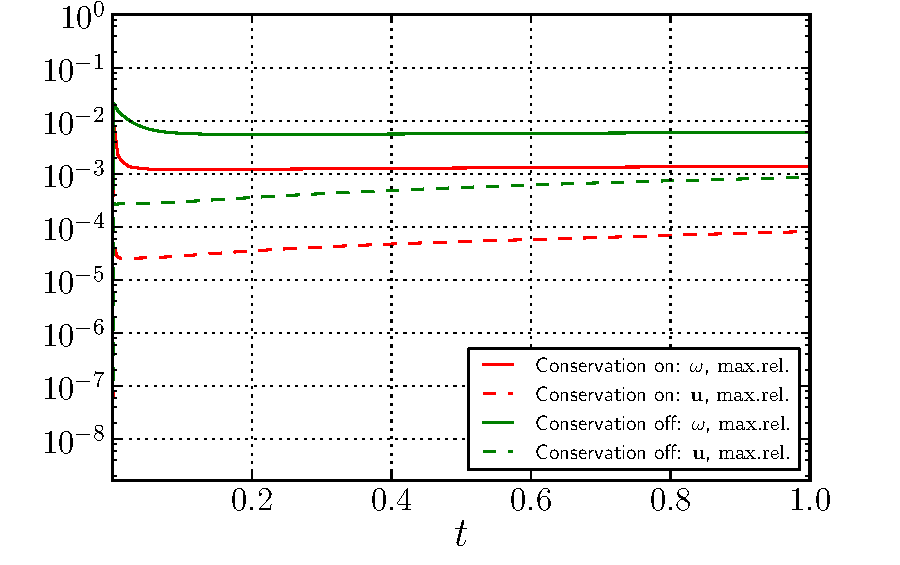
\includegraphics[width=0.6\linewidth]{./figures/validation/lambOseent2/lambOseen_comparision_conservation_compressed.pdf}
	\caption{Plot of the maximum relative error in vorticity $\epsilon_{\omega}$ [ - -, dashed] and maximum relative error in vorticity $\epsilon_{\mathbf{u}}$ [ ---, solid], equation \ref{eq:maxRelErrorDef}, from $t=0$ to $t=1$, using the parameters tabulated in table \ref{tab:HLO_pt}. The figure compares the coupling scheme with conservation of circulation ({\color{plotRed}{\textbf{red}}}) vs. the coupling scheme without conservation of circulation ({\color{plotGreen}{\textbf{green}}}).}
	\label{fig:lambOseen_comparision_conservation}
	\end{figure}	

	\begin{figure}[!p]
	\centering
	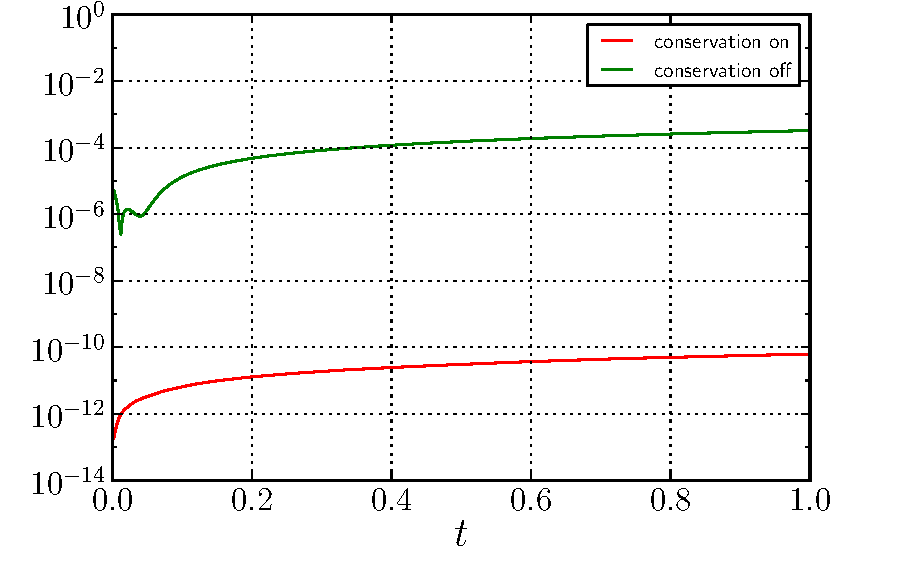
\includegraphics[width=0.6\linewidth]{./figures/validation/lambOseent2/lambOseen_comparision_conservation_circulation_compressed.pdf}
	\caption{Plot of the error in total circulation $\epsilon_{\Gamma}$ of the Lagrangian method from $t=0$ to $t=1$. The figure compares the scheme with conservation of circulation [ {\color{plotRed}{\textbf{---}}}, solid {\color{plotRed}{\textbf{red}}}], and the scheme without conservation of circulation [ {\color{plotGreen}{\textbf{---}}}, solid {\color{plotGreen}{\textbf{green}}}].}
	\label{fig:lambOseen_comparision_conservation_circulation}
	\end{figure}	
	

Figure \ref{fig:lambOseen_conservation_contourf} compares the error in the Eulerian domain $\Omega_E$ of the coupling approach without the conservation circulation against the approach satisfying the conservation of circulation, at $t=1$. We see that the scheme without the conservation has significantly larger error than the scheme with conservation. The maximum error is near the Eulerian boundary $\Sigma_d$ and shows an increase in the artificial vorticity emanating from the boundary due to the larger mismatch in the solutions, Figure \ref{fig:lambOseen_fullyCoff_wErrorFinal}. However, when we ensure that circulation is conserved, Figure \ref{fig:lambOseen_fullyCon_wErrorFinal}, the boundary produces significantly less error.


	

Figure \ref{fig:lambOseen_comparision_conservation} shows the evolution of the maximum relative error from $t=0$ to $t=1$, comparing the results of with and without the conservation of circulation. Observing the difference in the relative error in velocity and vorticity, we see that the scheme without the conservation of circulation produces larger errors at all times $t$. At $t=1$, we observe that the scheme without the conservation of circulation has a relative error in vorticity near \num{e-2}, whereas with the conservation of circulation, the relative error is an order of magnitude lower, reaching only \num{e-3}. Similarly for velocity, the scheme without the conservation of circulation has the relative error approaching \num{e-3}, whereas with the conservation enabled, the error only reaches \num{e-4}. 

Figure \ref{fig:lambOseen_comparision_conservation_circulation} shows the change in total circulation from $t=0$ to $t=1$ for the non-conserved and conserved scheme. It is apparent that without the conservation of circulation, the error in total circulation is significantly larger and approaches \num{e-3}. If the circulation is not conserved explicitly, the transfer of vorticity from the Eulerian method to the Lagrangian method introduces additional error in total circulation. By ensuring conservation of circulation, as described in section \ref{subsec:coupling-cotc}, we see that the error in total circulation is significantly smaller, near \num{e-10}. %It is to be noted that there will be still a linear increase in the total circulation is due to the population control of the vortex blobs, removing the circulation $\Gamma_{glob}$ at every evaluation, as described in section \ref{subsubsec:srs}.

Thus, we have determined that another potential source of error during the coupling of the two methods is the mismatch in the circulation. If we do not ensure conservation of circulation, the error in coupling is reflected by generation of large artificial vorticity, emanating from the outer Eulerian boundary $\Sigma_o$. The results validates this observation and therefore the algorithm described in section \ref{subsec:coupling-cotc} is vital for valid hybrid scheme.

\subsubsection{Parameter sensitivity analysis}
\label{subsubsec:psa}

The final question we have to answer is how discretization effects the coupling process. To determine this we varied the spatial and temporal resolution of the Lagrangian method and quantified the increase in the error. 

	\begin{figure}[!b]
	\centering
	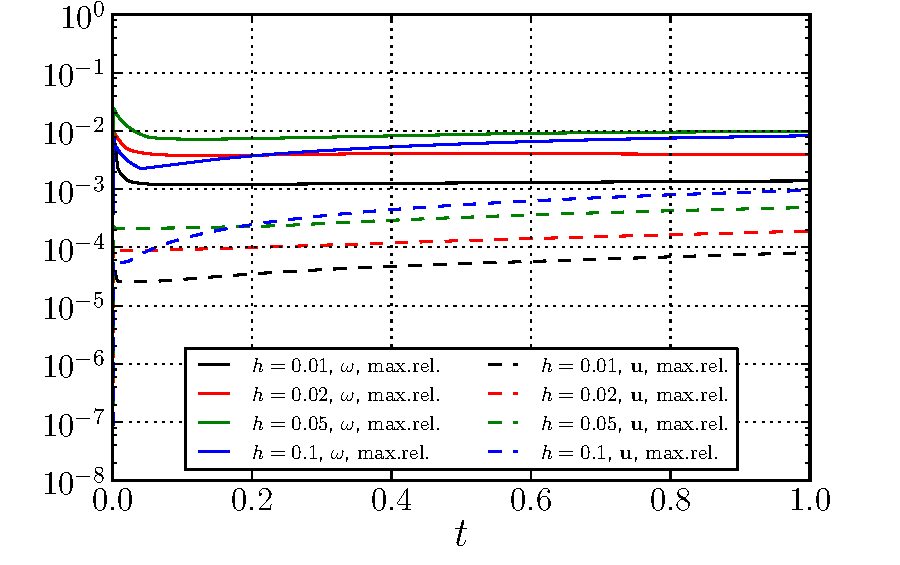
\includegraphics[width=0.6\linewidth]{./figures/validation/lambOseen/lambOseen_parameter_h.pdf}
	\caption{Evolution of the maximum relative error for various nominal blob spacing $h = [0.01,0.02,0.05,0.1]$ from $t=0$ to $t=1$.} %The figures shows the maximum relative error in vorticity [ - -, dashed] and maximum relative error in vorticity [ ---, solid].}
	\label{fig:lambOseen_parameter_h}
	\end{figure}

	\begin{figure}[!p]
	\centering
	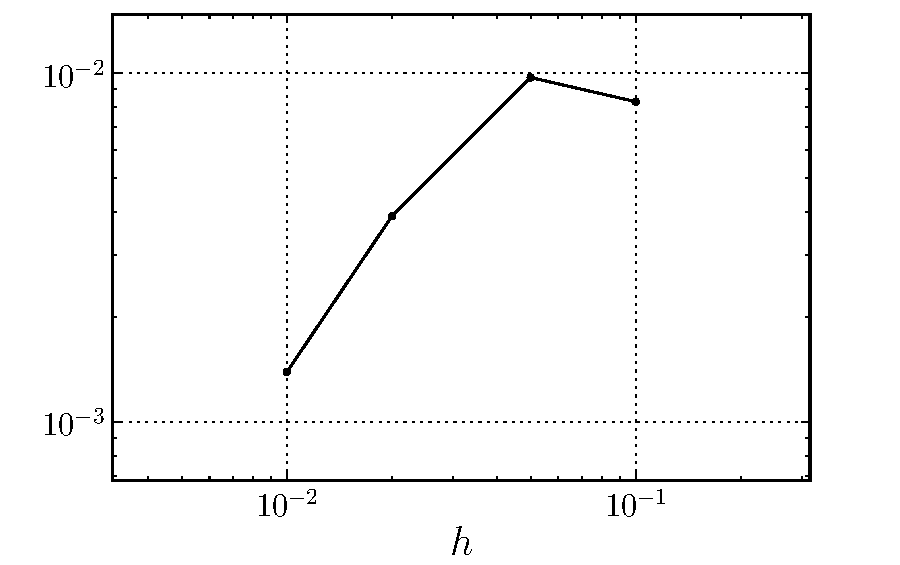
\includegraphics[width=0.6\linewidth]{./figures/validation/lambOseen/lambOseen_parameter_h_Trend.pdf}
	\caption{Convergence of the maximum relative error in vorticity due to the nominal blob spacing $h = [0.01,0.02,0.05,0.1]$.}
	\label{fig:lambOseen_parameter_h_Trend}
	\end{figure}
	
	\begin{figure}[!p]
	\centering
	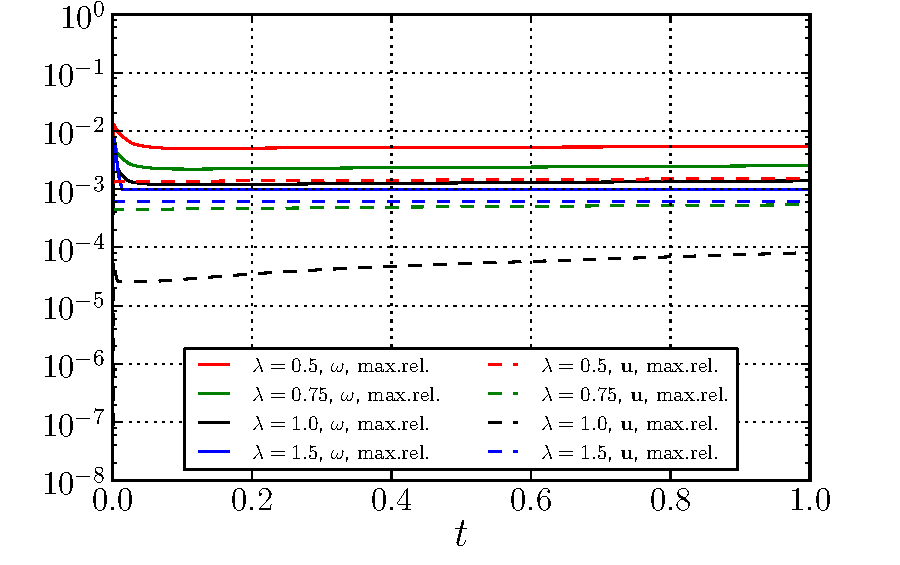
\includegraphics[width=0.6\linewidth]{./figures/validation/lambOseen/lambOseen_parameter_overlap.pdf}
	\caption{Evolution of the maximum relative error for various overlap ratios $\lambda = [0.5, 0.75, 1.0, 1.5]$ from $t=0$ to $t=1$. The figures shows the maximum relative error in vorticity [ - -, dashed] and the maximum relative error in vorticity [ ---, solid].}
	\label{fig:lambOseen_parameter_overlap}
	\end{figure}		

	\begin{figure}[!p]
     \centering
     \begin{subfigure}[t]{0.45\textwidth}
             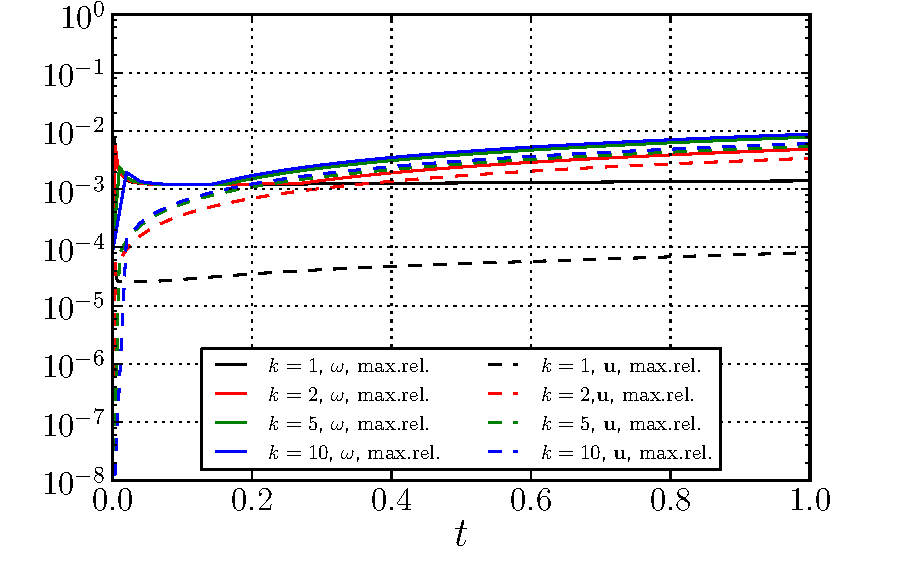
\includegraphics[width=\linewidth]{./figures/validation/lambOseen/lambOseen_parameter_k.pdf}
             \caption{$\Delta t_L = [0.001,0.002,0.005,0.01]$, $\Delta t_E = 0.001$}
             \label{fig:lambOseen_parameter_k_dtL}
     \end{subfigure}     
     \qquad
     \begin{subfigure}[t]{0.45\textwidth}
             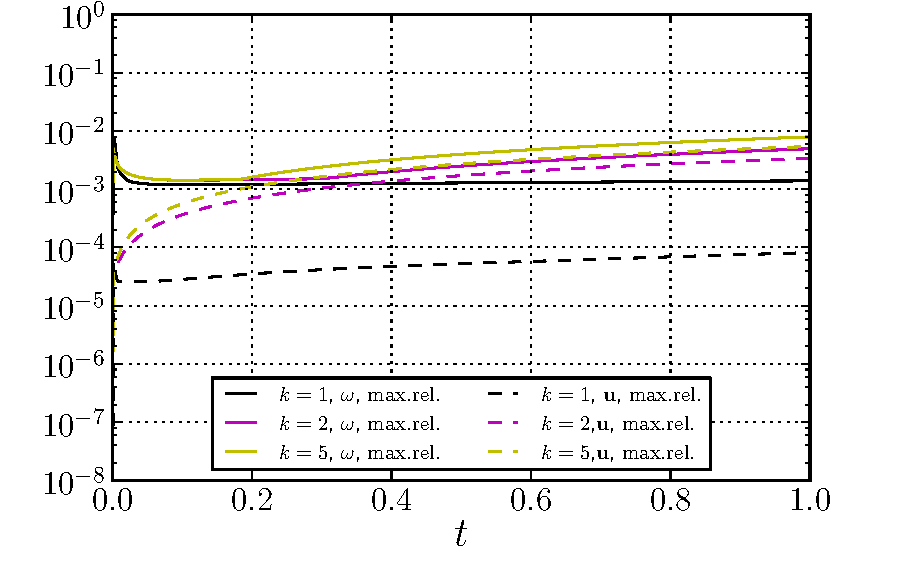
\includegraphics[width=\linewidth]{./figures/validation/lambOseen/lambOseen_parameter_k_dtE.pdf}
             \caption{$\Delta t_E = [0.001,0.0005,0.0002]$, $\Delta t_L = 0.001$}
             \label{fig:lambOseen_parameter_k_dtE}
     \end{subfigure}        
     
     \caption{Evolution of the maximum relative error from $t=0$ to $t=1$ for various number of Eulerian sub-steps $k_E = [1,2,5,10]$, modifying (\textbf{a}) the Lagrangian time step $\Delta t_L$, and (\textbf{b}) the Eulerian time step $\Delta t_E$. The figures shows the maximum relative error in vorticity [ - -, dashed] and maximum relative error in vorticity [ ---, solid].}
     \label{fig:lambOseen_parameter_k}
	\end{figure}

The spatial discretization of the Lagrangian method was modified by varying the nominal blob spacing $h$ and the overlap ratio $\lambda$. The temporal discretization was modified by varying the Lagrangian time step size $\Delta t_L$. The control variables of the simulations are the ones tabulated in table \ref{tab:HLO_pt}.




%The parameter sensitivity analysis is the last stage of the Lamb-Oseen vortex investigation. The Lamb-Oseen vortex test case was ideal to determining the effects of the temporal and the spatial discretization of the hybrid method on the accuracy of the coupling. 

	
	
Figure \ref{fig:lambOseen_parameter_h} shows the impact of varying the nominal blob spacing $h$ on the coupling. The maximum relative error in vorticity and the maximum relative error in velocity is plotted from $t=0$ to $t=1$ for nominal blob spacing $h = [0.01,0.02,0.05,0.1]$. The figure shows that increasing the spatial resolution of the Lagrangian method reduces the error. At $t=1$, the minimum error is observed for $h=0.01$ with the relative error in velocity at \num{e-4} and the relative error in vorticity at \num{e-3}. The maximum relative error is observed for $h=0.1$, with \num{e-3} for relative error in velocity and \num{e-2} for relative error in vorticity. This implies that the growth in error is of order one. Figure \ref{fig:lambOseen_parameter_h_Trend} shows the variation in the maximum relative error in vorticity at $t=1$ for various nominal blob spacing $h$. The figure indeed shows that the change in error due to the spatial discretization is of order one.

	


Figure \ref{fig:lambOseen_parameter_overlap} compares the evolution of the maximum relative error for various overlap ratios, $\lambda = [0.5, 0.75, 1.0, 1.5]$. We see that the minimum error in velocity and vorticity is observed for the overlap ratio $\lambda = 1$. As we move from this value, an increase in the error is observable. In section \ref{subsubsec:convergenceInterpolation}, we determined that to reduce the Gaussian blurring of the vorticity field from the Gaussian vortex kernels, we require an overlap ratio $\lambda=1$ and a small nominal blob spacing $h$. The parameter sensitivity analysis on the spatial discretization validates this observation and states that to ensure minimum error in coupling, these criteria has to be satisfied.

Figure \ref{fig:lambOseen_parameter_k_dtL} shows the effect of modifying the Lagrangian time step size $\Delta t_L$ w.r.t a fixed Eulerian time step size. With $\Delta t_E=0.001$ and the number of Eulerian sub-steps $k_E = [1,2,5,10]$, the Lagrangian time steps become $\Delta t_L = k_E\cdot\Delta t_E = [0.001,0.002,0.005,0.01]$. In Figure \ref{fig:lambOseen_parameter_k_dtE}, we instead vary the Eulerian time step $\Delta t_E = \Delta t_L/k_E = [0.001,0.0005,0.0002]$, with $\Delta t_L=0.001$ and $k_E = [1,2,5]$. We see that the error in coupling reduces as the resolution of the time discretization matches with each other, when $k_E = 1$. We see that when we use a higher number of Eulerian sub-step, regardless of varying the Lagrangian or the Eulerian time step, there is an increase in the error in coupling. 

%We see that the minimum error occurs when the time steps match (i.e $\Delta t_L = \Delta t_E$). However if increase the number of Eulerian time steps from $k_E = 1 $ to $k_E=2$, there an substantial increase in the relative error in velocity. This observation states that the linear interpolation used for sub-stepping process, has potential for improvement. A possible solution might be to employ a higher-order interpolation method for determining the Eulerian Dirichlet boundary condition at the sub-steps.

%Figure \ref{fig:lambOseen_parameter_k_Trend} shows the convergence trend of error in vorticity due to number of Eulerian sub-step $k_E$. 
%
%	\begin{figure}[!h]
%	\centering
%	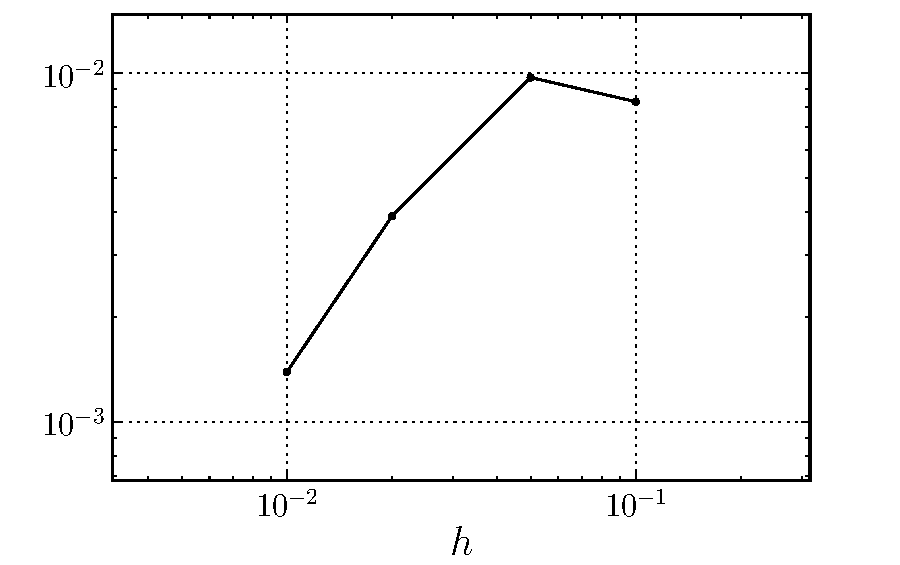
\includegraphics[width=0.6\linewidth]{./figures/validation/lambOseen/lambOseen_parameter_h_Trend.pdf}
%	\caption{Convergence of the error in coupling due to the number of Eulerian sub-step $k_E$ at $t=1$. The control variables are tabulated in table \ref{tab:HLO_pt}}.
%	\label{fig:lambOseen_parameter_k_Trend}
%	\end{figure}

\subsection{Conclusion}

In section \ref{subsec:UvOvF}, we observed that moving from uncoupled to one-way coupled case, increases the relative error in velocity. The growth in error was mainly due to the time integration error of the Lagrangian method. When moving from one-way coupled to fully coupled scheme, there is a tangible increase in the relative error in vorticity and an additional increase in the error in velocity. The increase in this error was due to the re-initialization of the vortex blobs introducing an additional smoothing error at each correction step. 

In section \ref{subsubsec:coc}, we observed that conservation of circulation is vital in ensuring an accurate coupling strategy. The transfer of vorticity from the Eulerian method to the Lagrangian method, must be performed with a focus on the conservation of circulation, to ensure that the artificial vorticity at the Eulerian Dirichlet boundary $\Sigma_d$ is minimal.

In section \ref{subsubsec:psa}, we investigated the impact of varying the spatial and temporal discretization on the accuracy of the coupling. We determined there is an increase in error, if the Lagrangian method is spatially under-resolved w.r.t to the Eulerian method. An overlap ratio of $\lambda=1$ was shown to have the minimum error during the coupling, as it ensures minimum Gaussian blurring. Varying the number of Eulerian sub-steps $k_E$, showed that the linear interpolation for the Dirichlet boundary condition is potential source of improvement.

Ultimately, the errors observed in the results can be explained and are consistent with the theory. We determined that in order to ensure a minimum error during the hybrid coupling, we must have a high spatial resolution at the zone of vorticity transfer (i.e the interpolation region $\Omega_I$), such that the discretization error of the two methods have minimum effect on the overall accuracy. Furthermore, we determined that conservation of circulation is vital to ensure correct transfer of solution between both methods and the algorithms described in section \ref{seec:coupling-mthlcs} are vital to ensure a proper Lagrangian correction step. 

\section{Clercx-Bruneau Dipole Convection}
\label{sec:vvhm-cbdc}

In section \ref{sec:vvhm-love}, we determined the source of the errors when coupling the Eulerian and the Lagrangian solution of ta Lamb-Oseen vortex diffusion case. However, an important aspect of domain decomposition method is the passage of a vortex core through a decomposed domain as it is a common phenomena in a VAWT simulation. As the blades pass through its own wake, they will encounter a shed vortex core from the previous blades. Therefore, the purpose of the Clercx-Bruneau dipole convection test cases is to determine whether the present hybrid method is capable of accurately describe a passage of a vortex core through a given Eulerian domain.

\subsection{Problem Definition}

To simulate the travel of a vortex core, we used the analytical expression of the Clercx-Bruneau dipole \cite{Clercx2006a} as the initial condition and simulated its convection through an Eulerian domain. The hybrid domain decomposition of this investigation is depicted in Figure \ref{fig:hcbconv_dd}. The Eulerian domain $\Omega_E$ is finite with bounds $[-0.25,0.25]\times[-0.5,0.5]$. The Clercx-Bruneau dipole, defined by equation \ref{fig:hcbconv_dd}, is initialized outside the Eulerian domain $\Omega_L\backslash\Omega_E$ at $(x_1,y_1) = (-1,0.1)$ and $(x_2,y_2)=(-1,-0.1)$, corresponding to the positive and negative cores, respectively. As the simulation progresses, the dipole convects along the $x$-axis, passing through the Eulerian domain.

	\begin{figure}[!h]
	\centering
	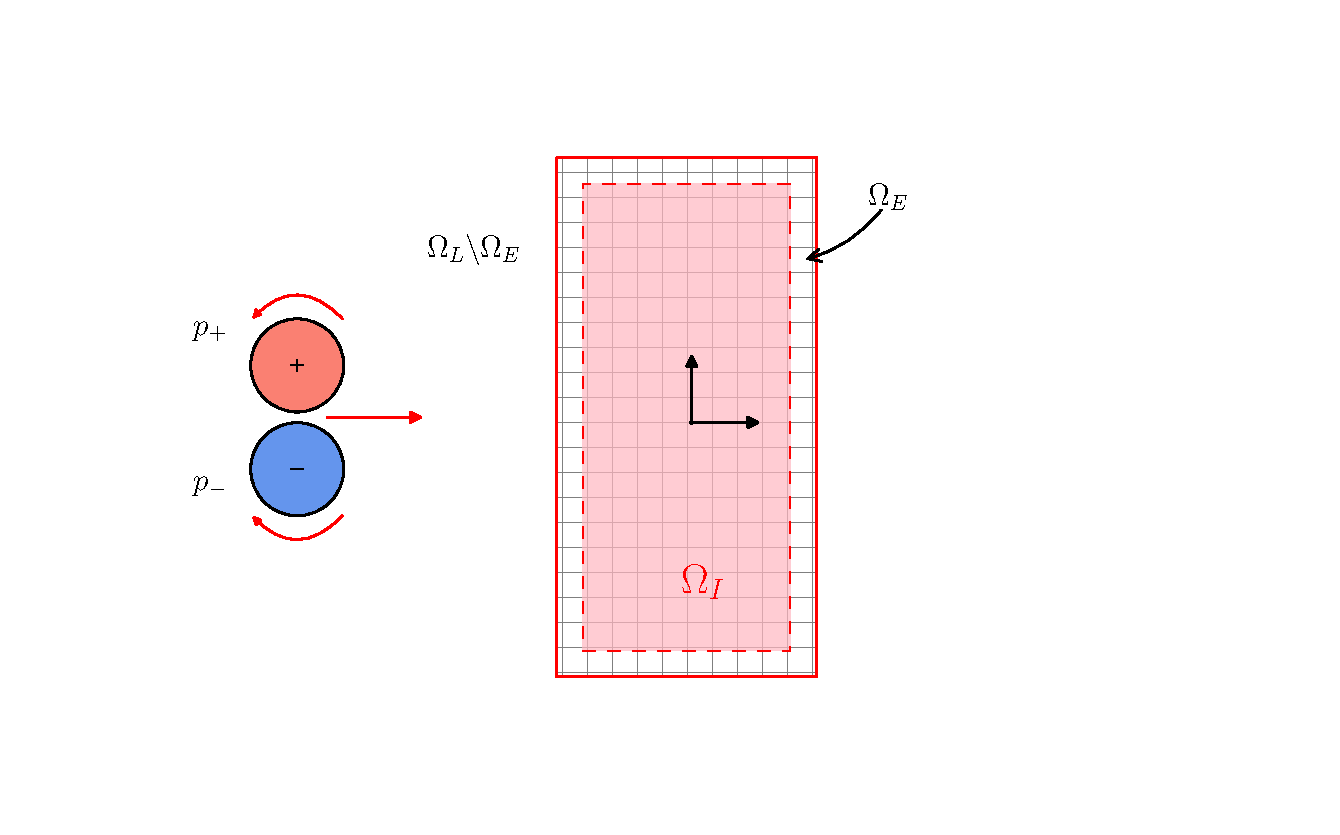
\includegraphics[trim=0cm 2.5cm 0cm 2.5cm, clip, width=\linewidth]{./figures/validation/cbConv/hcbconv_dd.pdf}
	\caption{(\textit{Not to Scale}) The domain decomposition for the Clercx-Bruneau convection problem, with the positive pole located at $p_{+}=(x_1,y_1) = (-1,0.1)$ and negative pole located at $p_{-}=(x_2,y_2)=(-1,-0.1)$. The parameters of the simulation are tabulated in table \ref{tab:HcbConvection_pt}.}
	\label{fig:hcbconv_dd}
	\end{figure}
	
The Eulerian and the Lagrangian domain are discretized according to the parameters shown in table \ref{tab:HcbConvection_pt}. The simulation was first benchmarked using a Finite Element (FE) only simulation, and a Vortex Particle Method (VPM) only simulation, providing an basis for hybrid simulation. To ensure that FE only simulation was valid, the Eulerian domain $\Omega_E$ spanned up to the far-field of the dipole, where the vorticity and the induced velocity are zero. The Eulerian domain $\Omega_E$ of the FE only simulation spanned $[-3,3]\times[-2,2]$. %For a valid comparison, these benchmark simulations followed similar parameters as the ones tabulated in table \ref{tab:HcbConvection_pt}.

	\ctable[
		caption = {Summary of the parameters for the Clercx-Bruneau dipole convection problem.},
		label   = {tab:HcbConvection_pt},
		pos = !t,]{lcll}{\tnote[a]{Obtained from Renac et al. \cite{Renac2013}}}{\FL
		
		Parameters 					& Value 	& Unit					& Description \ML
		$\Omega_E$             		& $[-0.25,0.25]\times[-0.5,0.5]$ &\si{m}	& Eulerian domain bounds \\
		$Re$						& 625 & - & Reynolds number\\
		$U$							& 1 & \si{m.s^{-1}} & Characteristic velocity\\
		$W$							& 1 & \si{m} & Characteristic Length\\
		$\nu$						& \num{1.6e-3} & \si{kg.s^{-1}.m^{-1}} & Kinematic viscosity\\
		$(x,y)_{1,2}$				& $(-1,\pm0.1)$ & \si{m} & Initial location of the monopoles\\
		$\omega_e$					& 299.528385375226\tmark[a] & - & Characteristic vorticity of the monopole\\
		$\lambda$					& 1 & - & Overlap ratio\\
		$h$							& 0.005 & \si{m} & Nominal blob spacing\\
		$h_{grid}$ 					& $\approx0.007$ & \si{m}	& FE cell diameter \\
		$ N_{\mathrm{cells}}$ 		& $40000$ 	& -						& Number of mesh cells\\
		$\Delta t_L$				& \num{2.5e-4} & \si{s} & Lagrangian time step size\\
		$\Delta t_E$				& \num{2.5e-5} & \si{s} & Eulerian time step size\\		
		$k_E$						& 10 & - & Eulerian sub-steps\\
		$ N_{\mathrm{t-steps}}$ 	& 2800 & -			& Number of time integration steps\\
		$t$							& 0 to 0.7 & - & Simulation time\\
		$d_{bdry}$					& $2\cdot{h}$ & \si{m} & Interpolation boundary offset\LL}


\subsection{Results}

	\begin{figure}[!t]
	\centering
	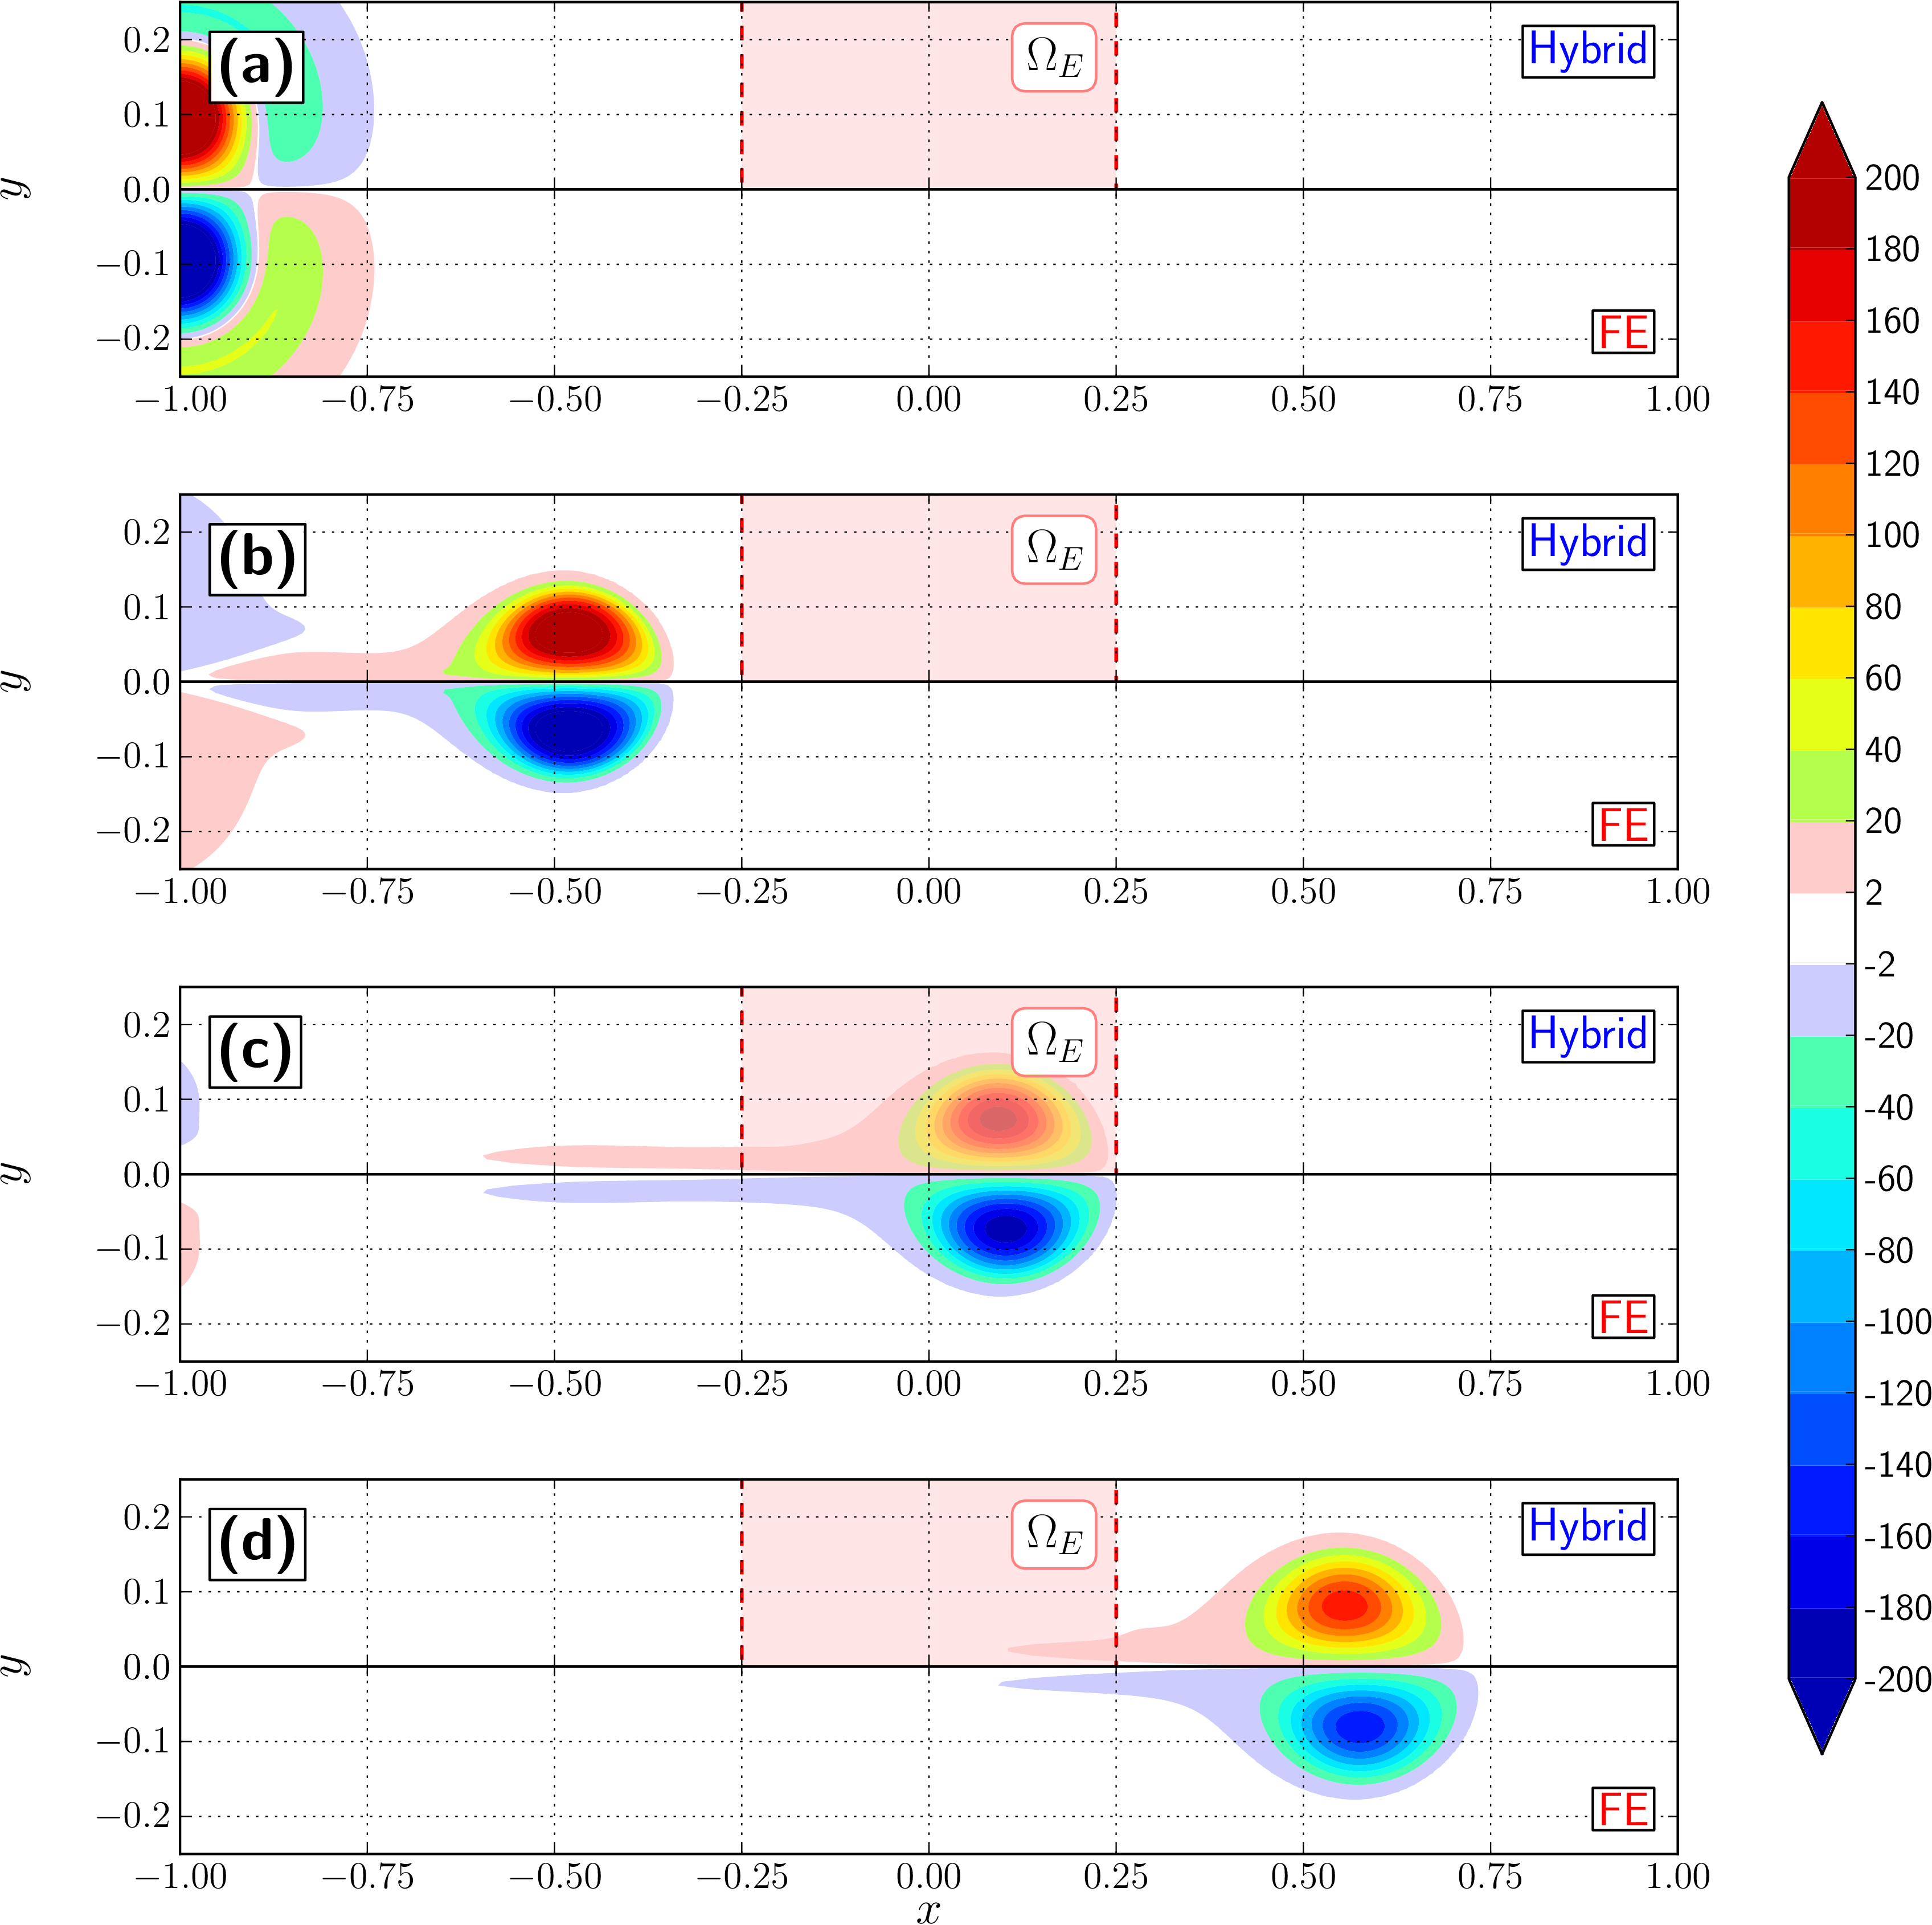
\includegraphics[width=\linewidth]{./figures/validation/cbConv/hybrid_doubleMonopoleConvection_contourfPlots-crop.png}
	\caption{Plot of the Clercx-Bruneau dipole at $t=[0,0.2,0.4,0.7]$ using parameters tabulated in table \ref{tab:HcbConvection_pt}. The figure compares the hybrid simulation (top halves) against the FE only simulation (bottom halves).}
	\label{fig:hybrid_doubleMonopoleConvection_contourfPlots}
	\end{figure}

	\begin{figure}[!t]
     \centering
     \begin{subfigure}[t]{0.48\textwidth}
             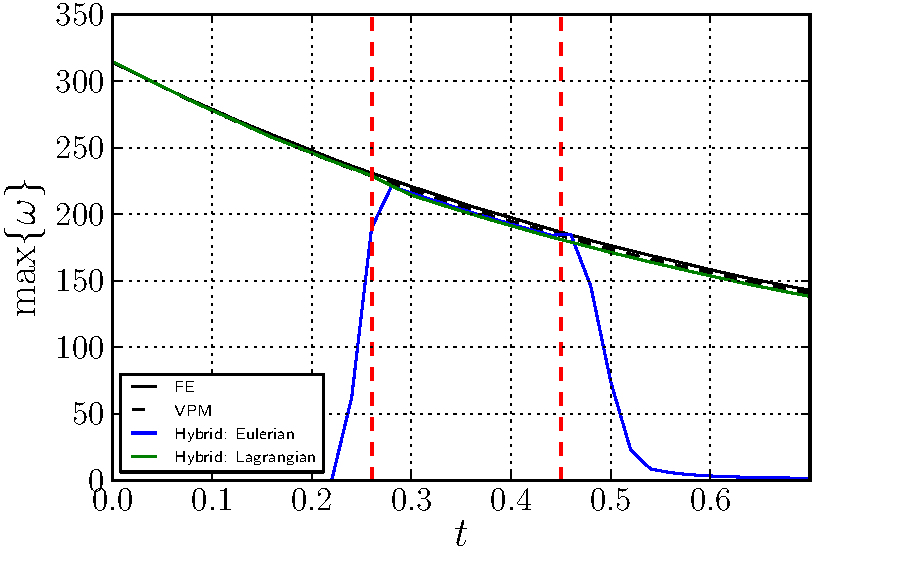
\includegraphics[width=\linewidth]{./figures/validation/cbConv/hybrid_dipoleConvection_hybridSubDomains_wMax.pdf}
             \caption{Comparison of the hybrid sub-domains}
             \label{fig:hybrid_dipoleConvection_hybridSubDomains_wMax}
     \end{subfigure}     
     ~ %\qquad
     \begin{subfigure}[t]{0.48\textwidth}
             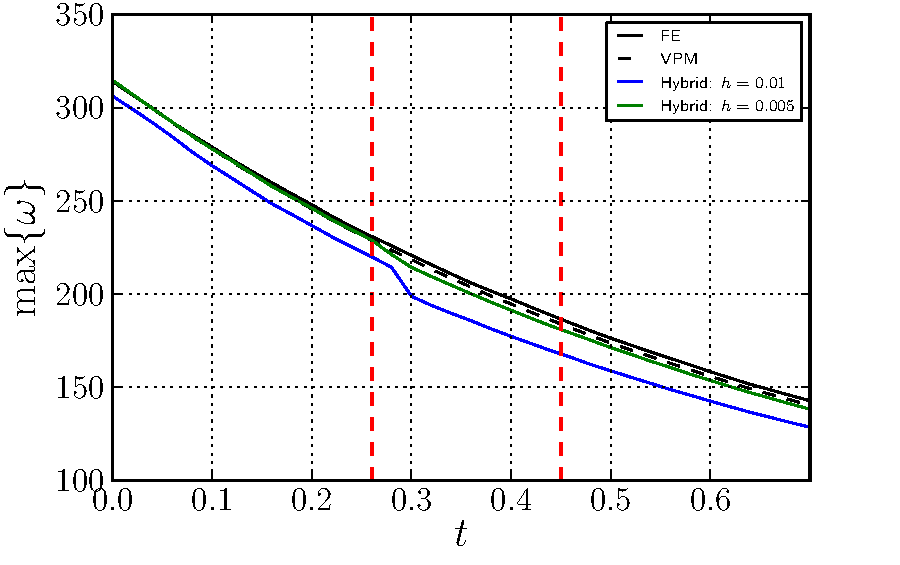
\includegraphics[width=\linewidth]{./figures/validation/cbConv/hybrid_dipoleConvection_comparison_parameter_wMax.pdf}
             \caption{Comparison with a less resolved hybrid method}
             \label{fig:hybrid_dipoleConvection_comparison_parameter_wMax}
     \end{subfigure}        
     
     \caption{Evolution of the maximum vorticity $\max\{\omega\}$ from $t=0$ to $t=0.7$. The solutions are compared with the benchmark results of FE only [---, solid black], and VPM only [- -, dashed black] simulations. The figure depicts (\textbf{a}) the maximum vorticity in the Eulerian and the Lagrangian sub-domain of the hybrid method, and (\textbf{b}) the maximum vorticity of hybrid method with nominal blob spacing $h=0.01$ and $h=0.005$.}
     \label{fig:hybrid_dipoleConvection_comparison_wMax}
	\end{figure}	
	
%	\begin{figure}[!p]
%     \centering
%     \begin{subfigure}[t]{0.48\textwidth}
%             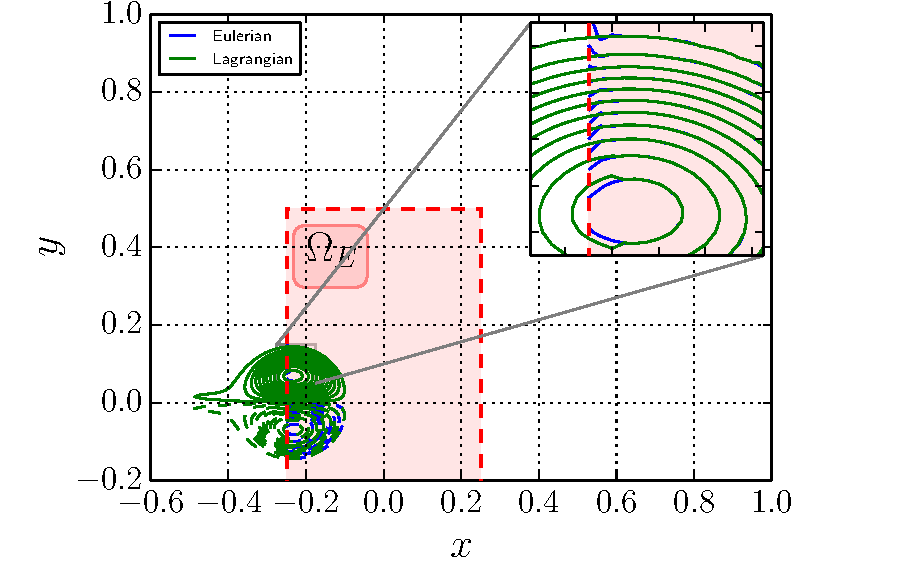
\includegraphics[width=\linewidth]{./figures/validation/cbConv/hybrid_doubleMonopoleConvection_entering2.pdf}
%             \caption{Entering at $t=0.26$}
%             \label{fig:hybrid_doubleMonopoleConvection_entering2}
%     \end{subfigure}     
%     ~ %\qquad
%     \begin{subfigure}[t]{0.48\textwidth}
%             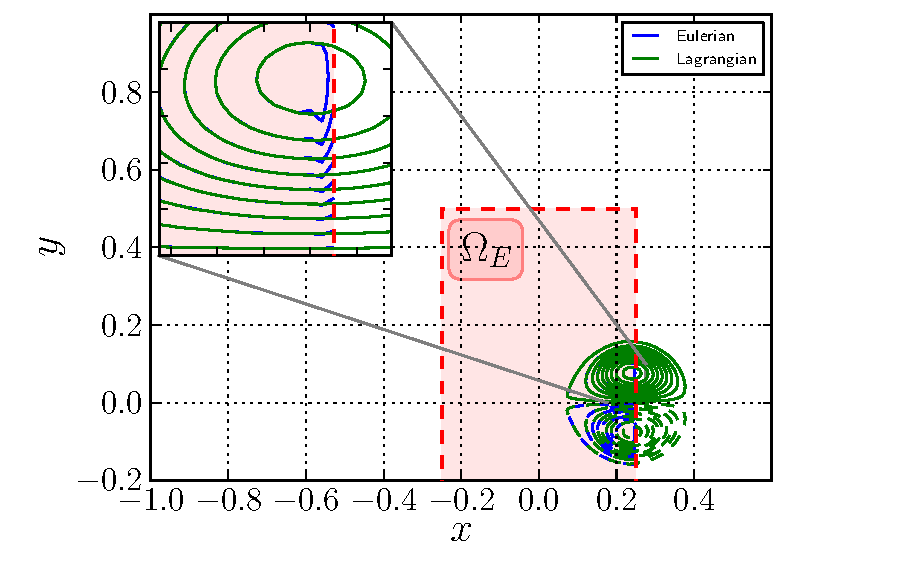
\includegraphics[width=\linewidth]{./figures/validation/cbConv/hybrid_doubleMonopoleConvection_exiting.pdf}
%             \caption{Exiting at $t=0.45$}
%             \label{fig:hybrid_doubleMonopoleConvection_exiting}
%     \end{subfigure}        
%     
%     \caption{Vorticity contour plots of the dipole with levels ...,-50,-30,-10,10,30,50,... of the Eulerian and the Lagrangian sub-domains. The figure highlights the effect of the artificial vorticity at the boundary of the Eulerian domain.}
%     \label{fig:hybrid_doubleMonopoleConvection_ent_exi}
%	\end{figure}
	
	\begin{figure}[!b]
     \centering
     \begin{subfigure}[t]{0.48\textwidth}
             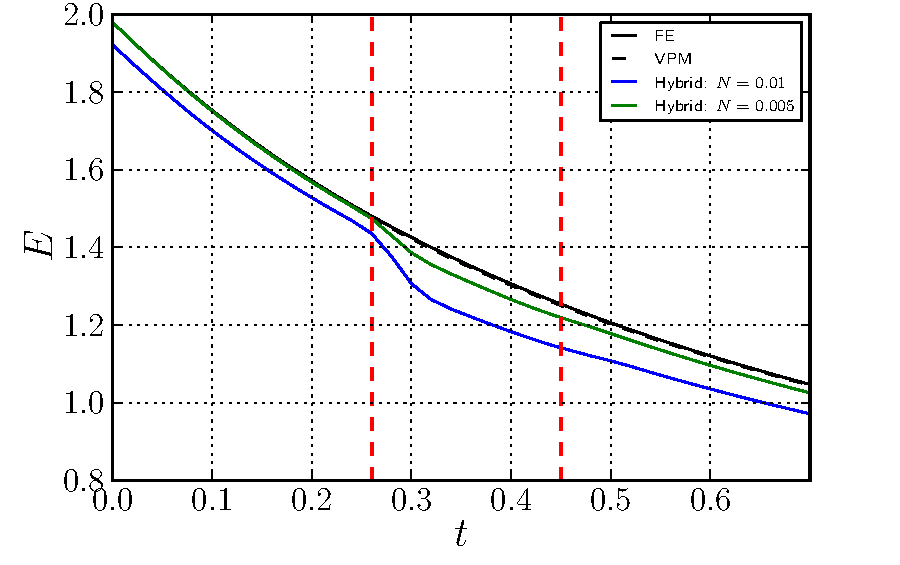
\includegraphics[width=\linewidth]{./figures/validation/cbConv/hybrid_dipoleConvection_comparison_parameter_E.pdf}
             \caption{Kinetic energy $E$}
             \label{fig:hybrid_dipoleConvection_comparison_parameter_E}
     \end{subfigure}     
     ~
     \begin{subfigure}[t]{0.48\textwidth}
             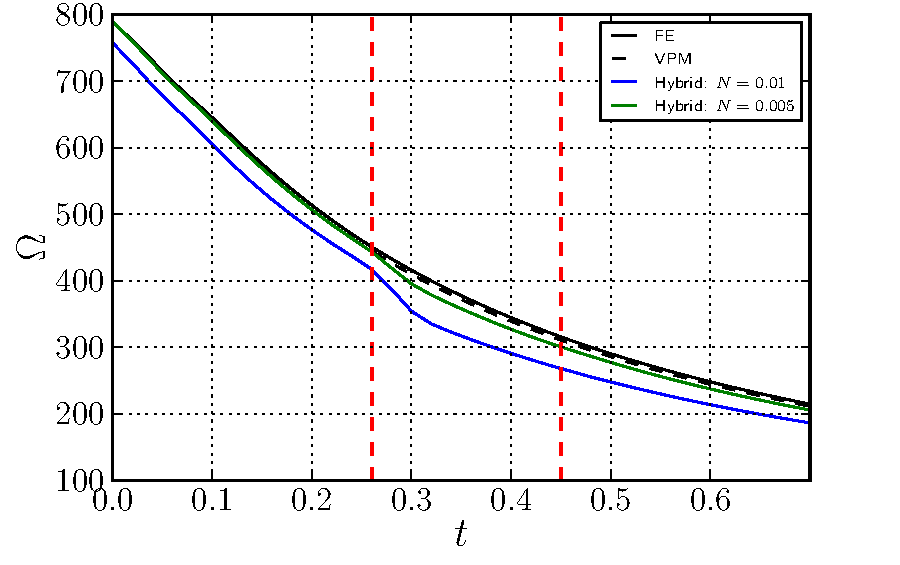
\includegraphics[width=\linewidth]{./figures/validation/cbConv/hybrid_dipoleConvection_comparison_parameter_Omega.pdf}
             \caption{Enstrophy $\Omega$}
             \label{fig:hybrid_dipoleConvection_comparison_parameter_Omega}
     \end{subfigure}        
     
     \caption{Evolution of the (\textbf{a}) kinetic energy $E$ and (\textbf{b}) enstrophy for the nominal blob spacing $h=0.01$ and $h=0.005$.}
     \label{fig:hybrid_dipoleConvection_comparison_parameter}
	\end{figure}
	
To determine whether the hybrid method was capable of accurate describe the passage of the Clercx-Bruneau dipole through the Eulerian domain, we first compared the plot of the vorticity field of the hybrid method with FE only simulation. Figure \ref{fig:hybrid_doubleMonopoleConvection_contourfPlots} compares the vorticity field of the FE simulation and the hybrid simulation at $t=[0,0.2,0.4,0.6]$. The top half of each subplot belongs to the hybrid simulation, whereas the bottom half to the FE only simulation. The cores of the dipole enters the Eulerian domain at $t=0.26$ and exits the domain at $t=0.45$. We see that the plot of the vorticity field matches till $t=0.7$. At $t=0.7$ however, the vorticity distribution in the hybrid method is lagging w.r.t the FE only simulation. 

%However in figure \ref{fig:hybrid_doubleMonopoleConvection_c ontourfPlots}c, the solutions start to deviate, and at $t=0.7$, figure \ref{fig:hybrid_doubleMonopoleConvection_contourfPlots}d, it is apparent that the dipole in the hybrid method is lagging w.r.t to the FE only simulation. This would imply that the passage of the vortex through the domain has a stalling influence on the vorticity evolution.

To investigate further on this influence of the passage, we analyzed variation in maximum vorticity $\omega_{max}$. Figure \ref{fig:hybrid_dipoleConvection_hybridSubDomains_wMax} shows evolution of the maximum vorticity $\omega_{max}$ from $t=0$ to $t=0.7$ in the Eulerian and the Lagrangian sub-domain of the hybrid simulation, the FE only simulation, and the VPM only simulation. At $t=0.26$, the maximum vorticity in the Eulerian sub-domain starts to increase, signifying the entering of the vortex core. Similarly, at $t=0.45$, the maximum vorticity starts to decrease, signifying the exiting of the vortex core. As the dipole enters the sub-domain, there is drop in the maximum vorticity. 
The explanation to this phenomena is the interaction of the artificial vorticity at the boundary $\Sigma_d$ with the solution. To confirm that influence of this artificial vorticity scales with the resolution of the simulation at the region of coupling (as concluded in section ??), we performed a simulation with lower resolution.

% in the vorticity in the Eulerian domain is the generation of the artificial vorticity. When the core of the dipole is right next the Eulerian boundary $\Sigma_d$, the influence of the vorticity on the boundary is larger. However, with the implementation of Stocks interpolation tolerance at the boundary, this artificial vorticity is somewhat neglected.
%A possible explanation to this phenomena might be error due to the artificial vorticity at the boundary. In section \ref{}, we observed that error in coupling introduces artificial vorticity at the boundary and the strength of this vorticity is proportional to the error in coupling. 
	
%Figure \ref{fig:hybrid_doubleMonopoleConvection_entering2} shows a vorticity contour plot of the Lagrangian method and the Eulerian method, at $t=0.28$ when the dipole has just entered the Eulerian domain. We see that there is a mismatch in the vorticity at the boundary of the Eulerian domain. Similarly, there is a slight mismatch in the vorticity field when the dipole leaves the Eulerian domain, figure \ref{fig:hybrid_doubleMonopoleConvection_exiting}.

Figure \ref{fig:hybrid_dipoleConvection_comparison_parameter_wMax} compares the evolution of maximum vorticity $\omega_{max}$ for nominal blob spacing $h=0.005$ and a lower resolution of $h=0.01$. We determine that the less resolved simulation indeed shows a larger drop in maximum vorticity, validating that the minimizing the artificial vorticity at boundary brings the accuracy hybrid simulation to the FE only simulation.

The evolution of the kinetic energy $E$ and the enstrophy $\Omega$ shows the similar behavior, Figures \ref{fig:hybrid_dipoleConvection_comparison_parameter_E} and Figure \ref{fig:hybrid_dipoleConvection_comparison_parameter_Omega}, respectively. The figures shows that with increasing spatial resolution, the hybrid simulation is able to simulate similar variation in flow parameters as the convection FE only or VPM only simulation. 

% shows that during the entry there is larger change in the kinetic energy and the enstrophy of the flow. The artificial vorticity causes an increased diffusion of the dipole. With the reduced strength of the vortex core, the dipole is weaker in energy and travels a shorter distance, as observed in figure \ref{fig:hybrid_doubleMonopoleConvection_contourfPlots}. The effect is more sever for a lower resolved Lagrangian method, as seen for the simulation with $h=0.01$.

\subsection{Discussion of results}

In conclusion, the results of the Clercx-Bruneau dipole convection simulation showed that:
\begin{itemize}
\item As the resolution of the hybrid method decreases at the overlap region, the effects of the artificial vorticity becomes greater.
\item A larger artificial vorticity at the boundary $\Sigma_d$, causes a greater lagging effect on the convection of the dipole.
\item A larger artificial vorticity at the boundary $\Sigma_d$, causes a larger reduction in the maximum vorticity $\omega_{\mathrm{max}}$, the kinetic energy $E$ and the enstrophy $\Omega$ at the entry of the dipole.
\end{itemize}

These results imply that for a less resolved Lagrangian method, the large artificial vorticity near the boundary has a significant diffusive effect on the vortex cores. The increased diffusion of the vortex cores causes the lagging phenomena and the larger drop in the maximum vorticity and the kinetic Energy. Therefore to accurate simulate the passage of a vortex core through the Eulerian domain, we need to minimize the influence of the artificial vorticity at the boundary. As the artificial vorticity is a representation of the difference in the Eulerian and the Lagrangian solution, we need to ensure that they have a matching discretization at the region of the overlap. Figure \ref{fig:hybrid_dipoleConvection_comparison_parameter_wMax} confirms this claim and shows that the effect reduces with matching discretization.

The results showed that with a matching spatial discretization, the hybrid method is indeed capable of simulating a passage of a dipole through the Eulerian domain. However, the limitation of the present study is that have not investigated in these finding are similar for different flow conditions such as:
\begin{itemize}
\item a higher Reynolds number
\item a large dipole convection velocity
\item a convection of a single monopole
\end{itemize}

These additional investigations could provide a stronger validation on whether the hybrid method is capable of simulation the passage of a vortex core through the decomposed Eulerian domain. Though, in the context of the present study, where we are concerned with laminar flow simulation, the understanding of the current investigation can be used for the other test cases.

%A suggestion to improve the validation of the vortex passage problem would be investigate for a higher Reynolds number, or a higher dipole convection velocity. However, for the present study as we are interested in a laminar regime simulations, the current dipole convection investigation should be valid for other test cases of the present study.

%In conclusion, we see that a high resolution discretization of the Lagrangian method inside the Eulerian domain $\Omega_L \cap \Omega_E$ is paramount for accurate transfer of information to and from the Eulerian method. For a lower resolved Lagrangian method in this region introduces artificial vorticity at the boundary of the Eulerian domain $\Sigma_d$, corrupting the solution of the coupling.

\section{Clercx-Bruneau Dipole Collision}
\label{sec:vvhm-cbdcoll}

In this section, we study the Clercx-Bruneau dipole colliding with a solid wall. The main goal this investigation is it determine if the hybrid method is able to accurately deal with a wall bounded problem. A Finite Element (FE) only investigation was first performed in section \ref{subsec:eul_cbdc} and was validated against the study of Clercx and Bruneau \cite{Clercx2006a}. We determined that the FE only simulation was able to provide results matching thel literature and therefore will be used as a benchmark for the present investigation.

\subsection{Problem Definition}

The setup of the hybrid domain is as shown in Figure \ref{fig:hcbdc_dd}. The Eulerian sub-domain $\Omega_E$ resolves the near-wall region, and the Lagrangian sub-domain domain resolves the complete fluid domain and is bounded by the no-slip wall $\Sigma_{w}$ (shown in blue). The Eulerian domain $\Omega_E$ extends from the wall $\Sigma_{w}$ to the boundary $\Sigma_{d}$, where the velocity boundary condition from the Lagrangian method is prescribed. The parameters of the simulation are tabulated in table \ref{tab:h_clercxBruneauParameters}.

	\begin{figure}[H]
	\centering
	%\includegraphics[trim=0cm 2.5cm 0cm 2.5cm, clip, width=\linewidth]
	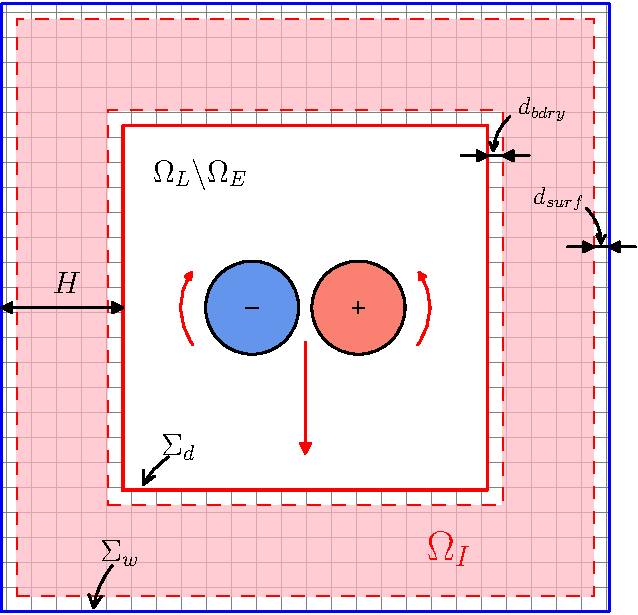
\includegraphics[width=0.6\linewidth]{./figures/validation/cbColl/hcbdc_dd-crop.pdf}
	\caption{[\textit{Not to Scale}] The domain decomposition for the Clercx-Bruneau dipole collision problem, with the positive pole at $p_{+}=(x_1,y_1) = (0.1,0)$ and negative pole at $p_{-}=(x_2,y_2)=(-0.1,0)$. The parameters of the simulation are tabulated in table \ref{tab:h_clercxBruneauParameters}.}
	\label{fig:hcbdc_dd}
	\end{figure}

	\ctable[
		caption = {Summary of the parameters for the Clercx-Bruneau dipole collision.},
		label   = {tab:h_clercxBruneauParameters},
		pos = !t,]{lcll}{\tnote[a]{Obtained from Renac et al. \cite{Renac2013}}}{\FL
		Parameters					& Value 				& Unit		& Description \ML
		$\Omega$               		& $\left[-1,1\right]^2$ &\si{m}		& Extend of Eulerian domain from wall $\Sigma_d$ \\
		$H$ & 0.2 & \si{m} & Eulerian domain width\\
		$Re$  			       		& $625$ 				&-			& Reynolds number \\ 
		$U$							& 1 & \si{m.s^{-1}} & Characteristic velocity\\
		$W$							& 1 & \si{m} & Characteristic Length\\
		$\nu$						& $\num{1.6e-3}$ 		&\si{kg.s^{-1}.m^{-1}}& Kinematic viscosity\\
		$ (x,y)_{1,2}$				& $(\pm0.1,0)$			& \si{m}    & Initial location of the dipole\\
		$\omega_e$					& 299.528385375226\tmark[a] & - & Characteristic vorticity of the monopole\\
		$\lambda$					& 1 & - & Overlap ratio\\
		$h$							& 0.003 & \si{m} & Nominal blob spacing\\
		$N_{panels}$ & 400 & - & Number of panels\\
		$h_{grid}$ 					& $0.005$ to $0.01$ & \si{m}	& FE cell diameter \\	
		$ N_{\mathrm{cells}}$ 		& $58272$ 	& -						& Number of mesh cells\\	
		$\Delta t_L$				& \num{2.5e-4} & \si{s} & Lagrangian time step size\\
		$\Delta t_E$				& \num{2.5e-5} & \si{s} & Eulerian time step size\\		
		$k_E$						& 10 & - & Eulerian sub-steps\\			
		$ N_{\mathrm{t-steps}}$ 	& 4000 & -			& Number of time integration steps\\
		$t$							& 0 to 1 & - & Simulation time\\
		$d_{bdry}$					& $2\cdot{h}$ & \si{m} & Interpolation domain offset from $\Sigma_d$\\
		$d_{surf}$					& $3\cdot{h}$ & \si{m} & Interpolation domain offset from $\Sigma_{w}$\LL}

As we are dealing with the wall-bounded problem, we require the vortex panel method to enforce the boundary condition in the Lagrangian method. In section \ref{subsec:hybrid-lcs}, we described the decomposition of the Lagrangian domain $\Omega_L$ into the vortex blob domain $\Omega_b$ and the vortex panel domain $\Omega_p$. Therefore, this decomposition was applied to this problem.

The dipole is initialized in the center of the domain, in the Lagrangian only domain $\Omega_L\backslash\Omega_E$ at the locations $(x,y)_{1,2}$. As the simulation progresses, the dipole travels along the negative $y$-axis, entering the Eulerian domain $\Omega$ and colliding with the no-slip wall $\Sigma_{w}$.

\subsection{Results}

The first step of the investigation was to compare the vorticity plots with the FE only simulation. Figure \ref{fig:hybrid_doubleMonolope_contourfComparison} shows the state of the dipole at $t=[0,0.2,0.4,0.6,0.8,1]$. The figure compares the hybrid simulation (left half) with the FE only simulation (right half), investigated in section \ref{subsec:eul_cbdc}. Onces the dipole enters the Eulerian domain, at $t=0.4$, we observe that there is a slight difference in the solution. The vorticity contours of $-10\leqslant \omega\leqslant-1$ (gray contours) and  $1\leqslant \omega\leqslant10$ (pink contours) shows that the near the core of the dipole there is a difference between the FE only simulation and the hybrid simulation. At $t=0.6$, we see there exists less vorticity in between $-1\leqslant1$ (white regions). The possible explanation of this behavior is the existence of the artificial vorticity. These artificial vorticity, which has a maximum absolute magnitude less than 5, has an effect on the vorticity profile of pink and gray vorticity contours. However, as the maximum absolute magnitude of the vorticity is $\max\{\omega\}=300$, the artificial vorticity is only $2\%$ of the maximum vorticity.

% We observe a slight artificial vorticity emanating from the Eulerian boundary $\Sigma_d$, corrupting the vorticity field. The corruption of the vorticity field is apparent when observing the hybrid plot at $t=0.4$, at the location $x=-0.2$ and $y=-0.8$. The artificial vorticity is in order of $<\pm5$. Note that with the maximum vorticity in the fluid near $\max\{\omega\}=300$ is near $2\%$ of the maximum vorticity.

Figure \ref{fig:hybrid_vorticity_contour_comparison} compares the vorticity contour at $t=1$ against the FE only simulation. We see there is a slight difference in the vorticity contour lines of hybrid solution, figure \ref{fig:hybrid_dipole_contourLine_t1p0}. The shape of the contour lines near the wall is slightly different, and furthermore, the location of the core is also shifted.

	\begin{figure}[!p]
	\centering
	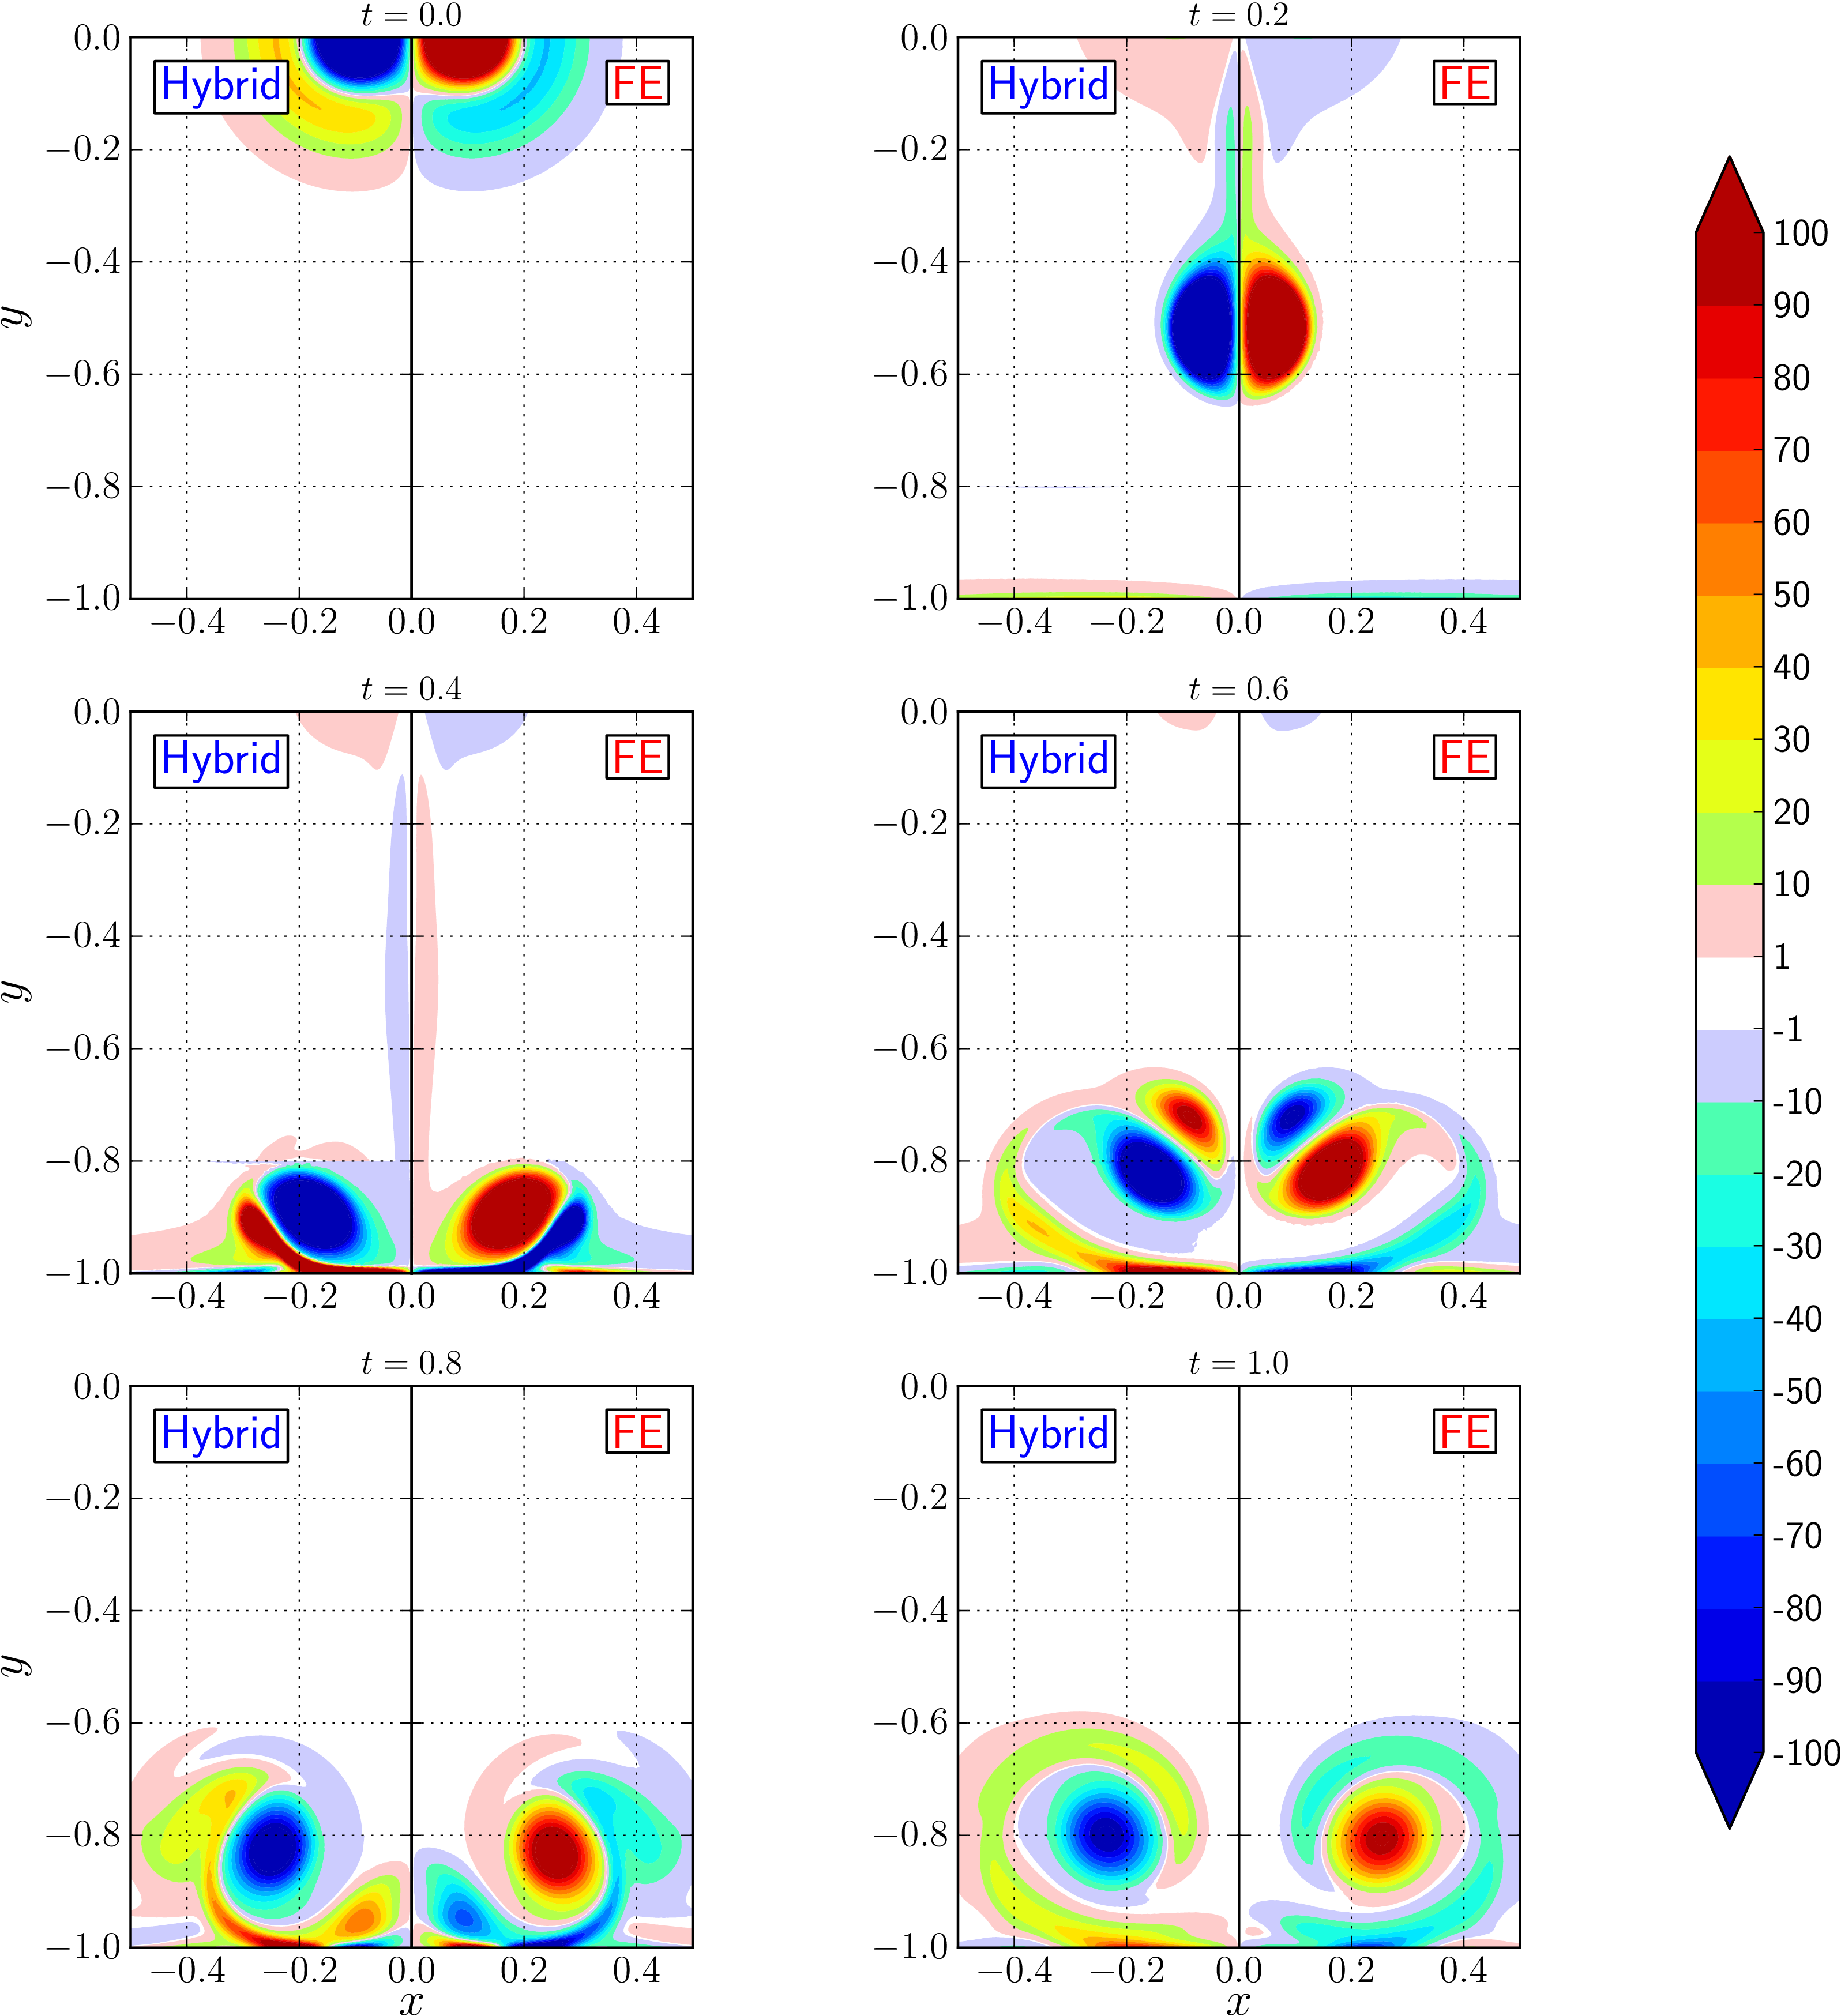
\includegraphics[width=\linewidth]{./figures/validation/cbColl/hybrid_doubleMonolope_contourfComparisonNew_compressed-crop.png}
	\caption{Plot of the dipole at $t = [0, 0.2, 0.4, 0.6, 0.8, 1]$, comparing the hybrid simulation (left half) and FE only simulation (right half).}
	\label{fig:hybrid_doubleMonolope_contourfComparison}
	\end{figure}

	\begin{figure}[!p]
     \centering
     \begin{subfigure}[t]{0.4\textwidth}
             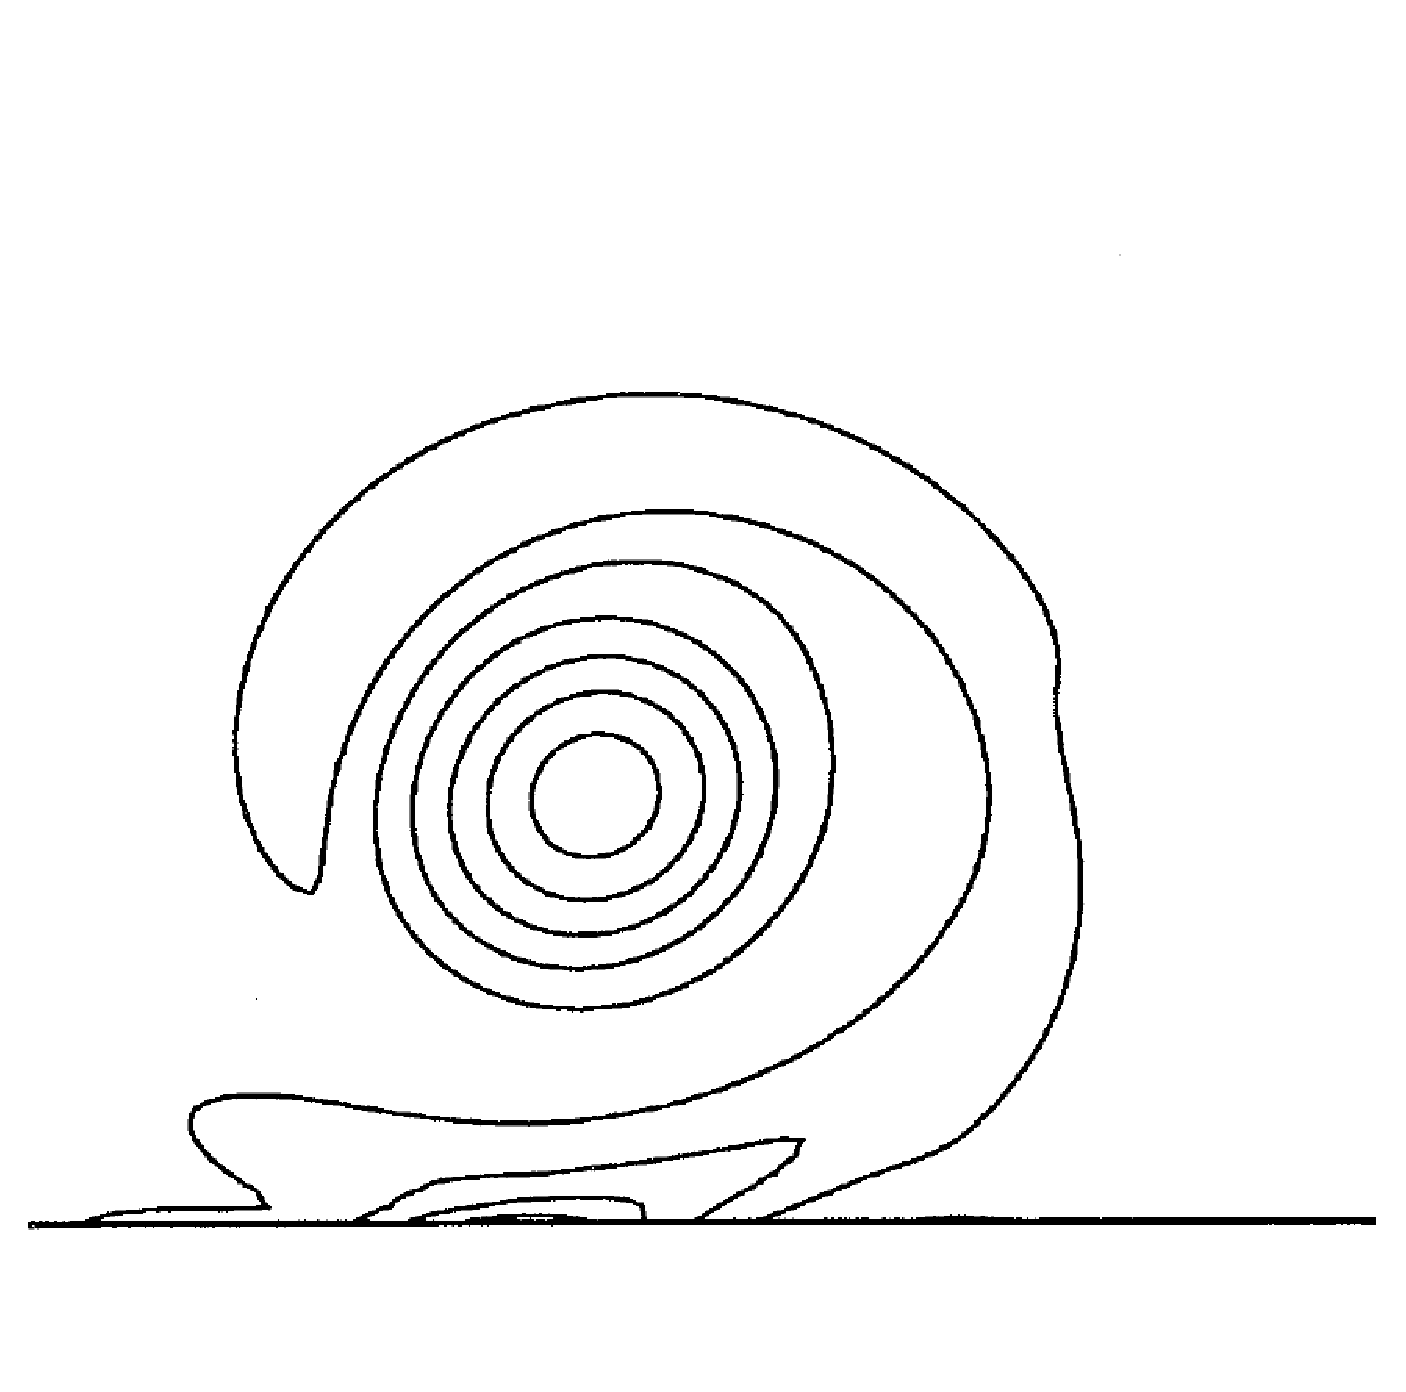
\includegraphics[width=\textwidth]{figures/eulerian/VorticityContourPlot-rotated270.pdf}
             \caption{Literature}
             \label{fig:hybrid_VorticityContourPlot}
     \end{subfigure}%
     ~ %add desired spacing between images, e. g. ~, \quad, \qquad etc.
       %(or a blank line to force the subfigure onto a new line)
     \begin{subfigure}[t]{0.5\textwidth}
             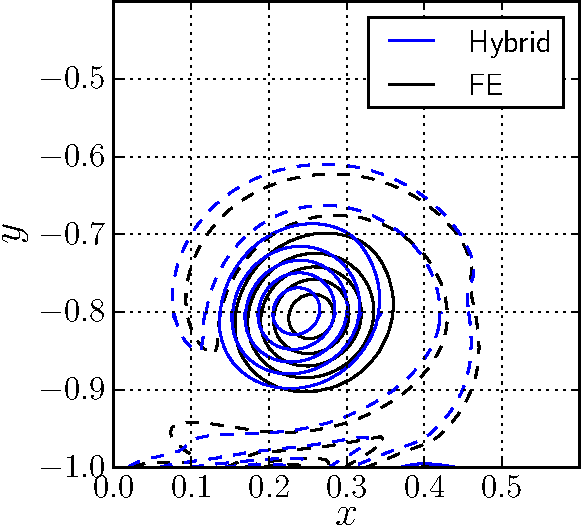
\includegraphics[width=\textwidth]{./figures/validation/cbColl/hybrid_doubleMonolope_contourComparison_t1-crop.pdf}
             \caption{Present study}
             \label{fig:hybrid_dipole_contourLine_t1p0}
     \end{subfigure}
     \caption{Comparison of the vorticity contours at $t=1$. The figure compares the plot obtained by \textbf{(a)} literature, Clercx and Bruneau \cite{Clercx2006a}, and \textbf{(b)} the present study, the hybrid and FE only simulation.}
     \label{fig:hybrid_vorticity_contour_comparison}
	\end{figure}	

	\begin{figure}[!p]
     \centering
     \begin{subfigure}[t]{0.49\textwidth}
             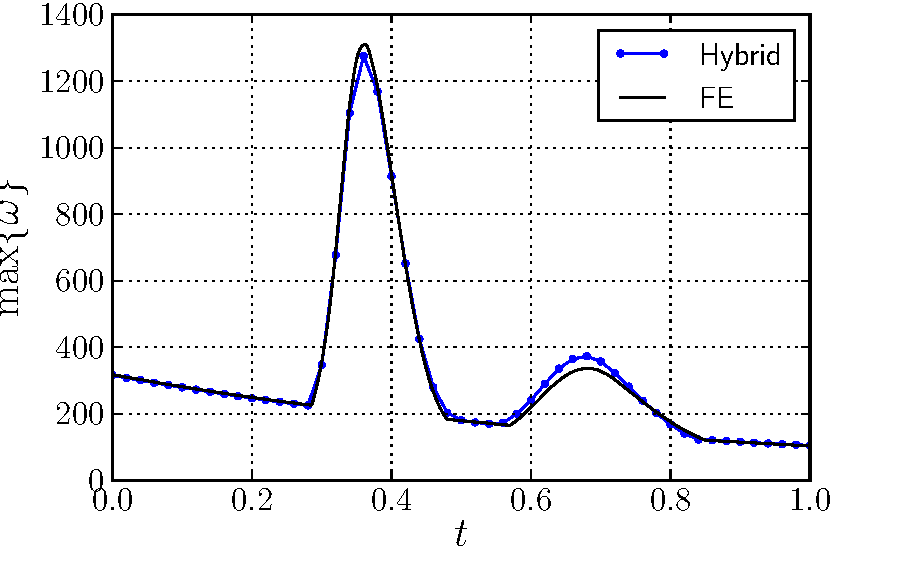
\includegraphics[width=\textwidth]{./figures/validation/cbColl/hybrid_doubleMonopole_parameter_wMax.pdf}
             \caption{Maximum vorticity $\max\{\omega\}$}
             \label{fig:hybrid_dipole_maxVorticity_comparison}
     \end{subfigure}%
     ~ %add desired spacing between images, e. g. ~, \quad, \qquad etc.
       %(or a blank line to force the subfigure onto a new line)
     \begin{subfigure}[t]{0.49\textwidth}
             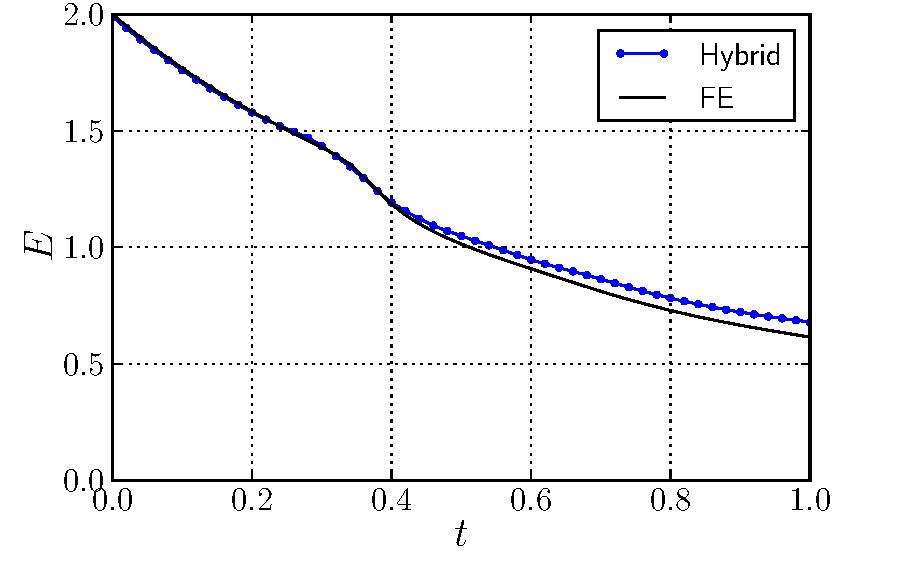
\includegraphics[width=\textwidth]{./figures/validation/cbColl/hybrid_doubleMonopole_parameter_E.pdf}
             \caption{Kinetic Energy $E(t)$}
             \label{fig:hybrid_dipole_KineticEnergy_comparison}
     \end{subfigure}
     
     \begin{subfigure}[b]{0.49\textwidth}
             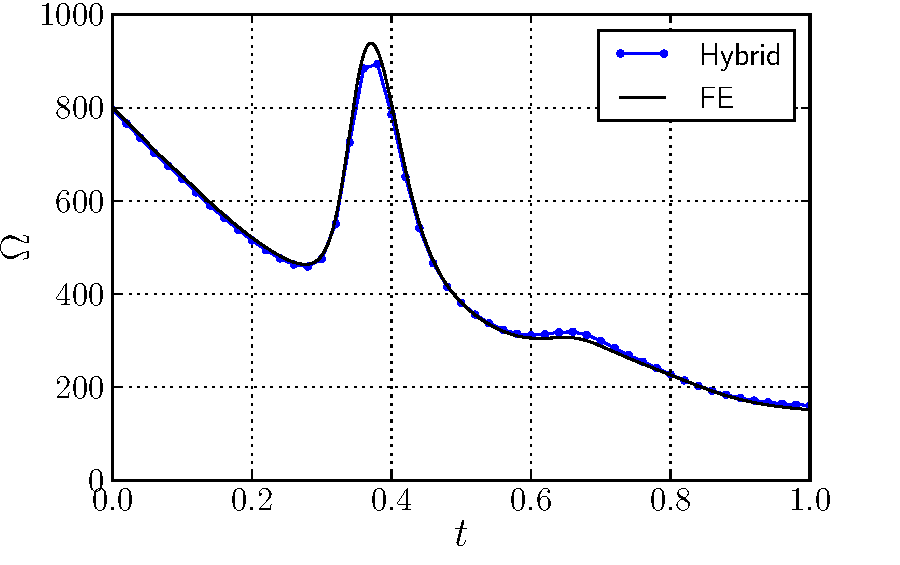
\includegraphics[width=\textwidth]{./figures/validation/cbColl/hybrid_doubleMonopole_parameter_Omega.pdf}
             \caption{Enstrophy $\Omega(t)$}
             \label{fig:hybrid_dipole_Enstrophy_comparison}
	 \end{subfigure}
     ~
	 \begin{subfigure}[b]{0.48\textwidth}
	 		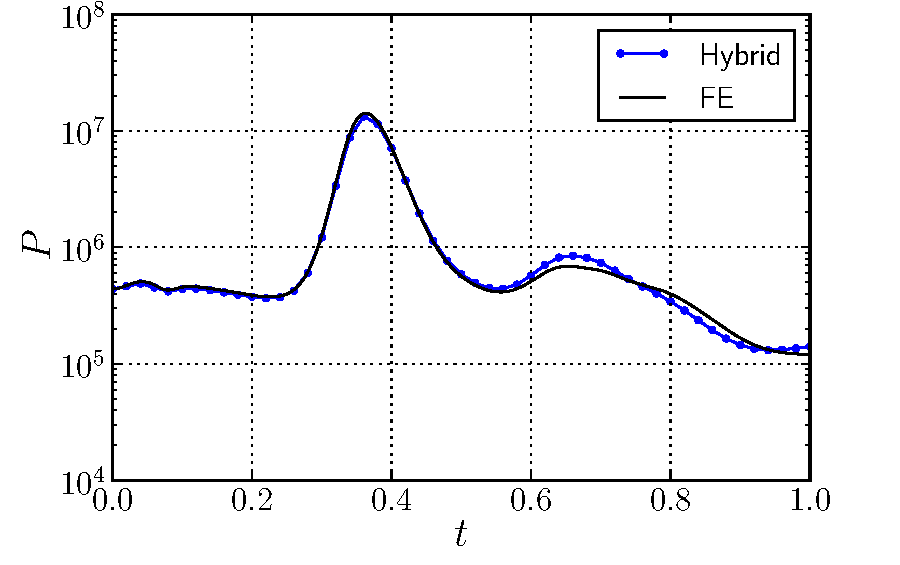
\includegraphics[width=\textwidth]{./figures/validation/cbColl/hybrid_doubleMonopole_parameter_P.pdf}
             \caption{Palinstrophy $P(t)$}
			\label{fig:hybrid_dipole_Palinstrophy_comparison}
	 \end{subfigure}     
     
     \caption{Variation in the fluid parameters from $t=0$ to $t=1$. The figure compares the hybrid results [{\color{plotBlue}{---}}, solid blue] with the FE only [---, solid black] results.} %Figure \textbf{(d)} compares the vorticity generated at the bottom-left wall ($y=-1$, $-0.6\leqslant x \leqslant 0$) at $t=0.4$ [{\color{plotBlue}{---}}, solid blue], $t=0.6$ [{\color{plotRed}{---}}, solid red] and $t=1$ [{\color{plotGreen}{---}}, solid green].}
     \label{fig:hybrid_dipole_comparison}
	\end{figure}

To investigate further on the cause of this difference, we studied the change in maximum vorticity $\omega_{max}$, the kinetic energy $E$, the enstrophy $\Omega$, and the palinstrophy $P$, shown in Figure \ref{fig:hybrid_dipole_Palinstrophy_comparison}. The variation in maximum vorticity, Figure \ref{fig:hybrid_dipole_maxVorticity_comparison}, shows that the first peak in the hybrid is nearly the same as FE only simulation, at $t\approx 0.35$. However, the second peak in vorticity, at $t\approx0.65$ is higher than the standard simulation. Between $t=0.4$ and $t=0.6$, the dipole exits and renters the Eulerian domain, as seen in Figure \ref{fig:hybrid_doubleMonolope_contourfComparison}. 

Figure \ref{fig:hybrid_dipole_KineticEnergy_comparison} shows that, as the dipole leaves the Eulerian domain $\Omega_E$ from $t=0.4$, the kinetic energy $E$ is higher. At $t=1$, the kinetic energy of hybrid is approximately 10\% higher than FE only simulation.

Investigating the enstrophy $\Omega$ , Figure \ref{fig:hybrid_dipole_Enstrophy_comparison}, and the palinstrophy $P$, we see that the difference is simulation is observable from only $t=0.6$. Therefore, the variation in the simulation only occurs from the second collision of the dipole, when dipole re-enters the Eulerian domain. Therefore the cause the deviation must be the result of dipole entering the Eulerian domain.

% less, and is higher than the FE only simulation at $t\leq0.4$. Therefore, the core that is leaving and re-entering the Eulerian domain $\Omega_E$ has a higher kinetic energy $E$. This could be cause of deviation seen at $t=1$, figure \ref{fig:hybrid_vorticity_contour_comparison}.

%Figure \ref{fig:hybrid_dipole_Enstrophy_comparison} shows that the enstrophy $\Omega$ matches reasonable well with the FE only simulation and we see that there is a slight difference at the peaks. Similarly, figure \ref{fig:hybrid_dipole_Palinstrophy_comparison}, shows the variation in palinstrophy $P$. The solution stars to deviate from $t\approx0.5$, after the vortex core re-enters the domain.

Due to the increased kinetic energy $E$, we see that there is slight difference in the distribution of the vorticity field along $y=-1$, Figure \ref{fig:hybrid_doubleMonopole_vorticityAtBoundary}. The figure shows when the kinetic energy of the simulations match, at $t=0.4$, the distribution of the vorticity is the same. However as time progresses, the difference in the shape of the distribution becomes apparent. At $t=1$, we see that the vorticity peak is wider and is due to the increased generation of vorticity from the wall to repel the dipole with higher kinetic energy $E$.

%or $t=0.4$ the solution matches, at $t=0.6$ the peak in vorticity is larger for the hybrid simulation, and for $t=1$, the peak has a larger span. The increased kinetic energy $E$ of the vortex could provide a possible explanation for this. With a higher kinetic energy, the wall generates stronger vorticity to repel the dipole.

	\begin{figure}[!t]
	\centering
	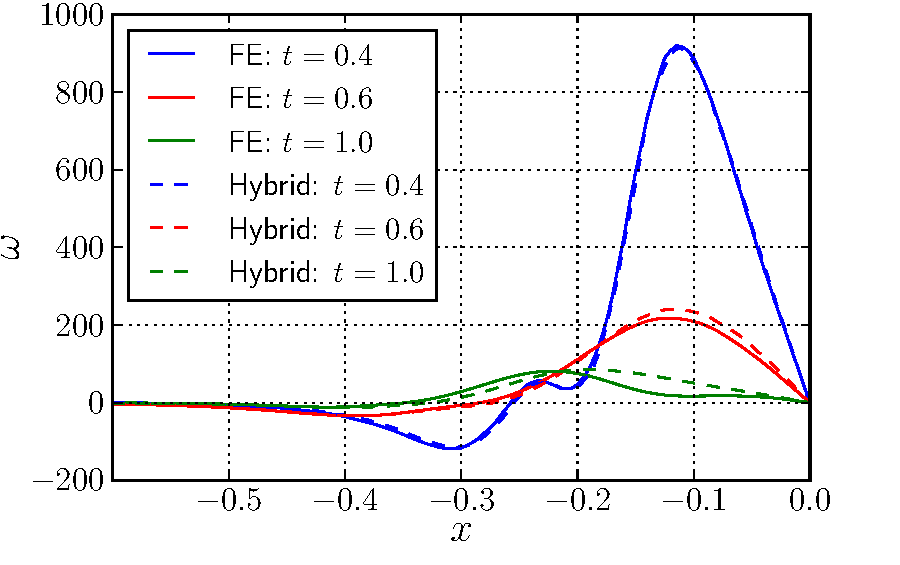
\includegraphics[width=0.5\linewidth]{./figures/validation/cbColl/hybrid_doubleMonopole_vorticityAtBoundary.pdf}
	\caption{Compares the vorticity generated at the bottom-left wall ($y=-1$, $-0.6\leqslant x \leqslant 0$) at $t=0.4$ [{\color{plotBlue}{---}}, blue], $t=0.6$ [{\color{plotRed}{---}}, red] and $t=1$ [{\color{plotGreen}{---}}, green].}
	\label{fig:hybrid_doubleMonopole_vorticityAtBoundary}
	\end{figure}

We investigated further with a higher resolved Lagrangian method, with a smaller nominal blob spacing $h$, a larger number of panels $N_{panels}$, and a smaller Lagrangian time step size $\Delta t_L$. However, these simulation did not provide significant improvement to the present results and was inconclusive. 
%Therefore, we see that the primary source of the error in not the resolution of the Lagrangian solution, but entering and re-entering of the vorticity into the Eulerian domain.


\subsection{Discussion of Results}

In conclusion, the results of the dipole collision simulation showed that:
\begin{itemize}
\item The hybrid method is capable of dealing with the no-slip boundary.
\item The results of the simulation are in good agreement upto $t=0.5$.
\item After $t=0.5$, when the dipole re-enters, the hybrid simulation starts to deviate due to the presence of artificial vorticity.
\item At $t=1$, due to the higher kinetic energy $E$ in flow, the location of the vortex core at $t=1$ is different.
\end{itemize}

The present investigation verified and validated that the algorithm for determine the vortex panel strength described in section \ref{seec:coupling-mthlcs} was capable of dealing with the no-slip boundary. The Eulerian method provided the necessary vorticity distribution into the fluid domain to oppose the oncoming dipole and the circulation of the vortex panels was determined directly from the Eulerian domain.

However, deviation with the hybrid simulation and the Eulerian simulation was observed was caused by the presence of the artificial vorticity.  With a boundary offset of $d_{bdry}=2\cdot{h}$, as used by Stock \cite{Stock2010a}, the present results were obtained. However, during further investigation with impulsively started cylinder in section \ref{sec:vvhm-isc}, we determined that using such a small offset results in the amplification of the effect of the artificial vorticity, resulting in the mismatch of the kinetic energy at $t=1$.

Therefore the limitation of the present test case is that it does not provide a full understanding of the collision of the dipole with the wall boundary. So, a simulation with various $d_{bdry}$ in future, can provide a more detailed understanding of the collision problem.

However, as the main purpose of this test case was to determine whether the hybrid method was capable of dealing with the wall boundary. The present test case provided this necessary confirmation and furthermore gave us an understanding of the potential inaccuracies, if the artificial vorticity if it is not dealt with.



%the coupling of the Lagrangian method (without a vorticity diffusion from the panel) and Eulerian method is able to simulate the collision of dipole with the no-slip wall. We observed that the Eulerian method provided the necessary vorticity distribution into the fluid domain to oppose the oncoming dipole. Furthermore, using the algorithm described in section \ref{seec:coupling-mthlcs}, we were able to determine the strengths of the vortex panels that satisfied the no-slip boundary condition and the total circulation.

%However, an issue with the present results was the effect of the artificial vorticity on the simulation. The present simulation used the boundary offset $d_{bdry}$ according to the literature of Stock \cite{Stock2010a}. However, in the later simulation, in section ??, we realized that our hybrid method required a larger offset from the boundary. Therefore the results of the present test case does not accurate depict the potential of the hybrid simulation. 

%Even though, we used a small $d_{bdry}$ cause an increased influence of the artificial vorticity, the results shows a similar behavior as the FE only simulation. The impact only become apparent after multiple re-entry of the dipole. Thus a suggestion for an improved understanding of how the hybrid method deals with a dipole collision, is to perform a additional investigations with various $d_{bdry}$.
%Though, due to the multiple re-entry of the dipole through the Eulerian outer boundary $\Sigma_o$, where we have artificial vorticity, there was an increase in the kinetic energy. The difference in the kinetic energy meant that there was a difference in the location of the vortex core at $t=1$.



%the boundary conditions of the Lagrangian method was able accurately calculated by simply using the approach described in section ??, where circulation of the vortex panels was determined from the Eulerian method and the no-slip boundary conditio

%wby only ensuring no-slip boundary condition on the vortex panels the boundary conditions of the Lagrangian method 

%As the dipole re-enters the Eulerian domain during the collision, the dipole passes through the region of artificial vorticity multiple times. 



%we determined that the exists a slight difference in the geometry of the vorticity contours and the location of the dipole at the end of the simulation. The deviation of the dipole stars as the dipole enters the Eulerian domain. The entering and the re-entering process of the dipole introduces artificial vorticity from the Dirichlet boundary $\Sigma_d$, increasing the overall kinetic energy $E$ of the problem. This intern has an influence on the position of the dipole at $t=1$. Increasing the resolution of the Lagrangian solution only minimally increases the accuracy of the results. 

%It is recommended that a further focused study should be performed on the artificial vorticity generated from the boundary of Eulerian domain $\Sigma_d$. If this artificial vorticity can be further minimized, we could potential attain more accurate results.

\section{Impulsively Started Cylinder at $Re=550$}
\label{sec:vvhm-isc}
In this section, we will study the flow around an \printAcron{impulsively started cylinder}{ISC} at $Re=550$. The purpose of this test case is ensure that we are able to correctly predict the lift and drag forces acting on a body. In section \ref{subsec:eul_isc}, the FE only simulation was validated against the study of Koumoutsakos and Leonard \cite{Koumoutsakos1995a}, and the study of Rosenfeld et al. \cite{MosheRosenFeldDochanKwak1991}. The FE only investigation will be therefore be used a benchmark for the current hybrid study.

\subsection{Problem Definition}

The description of the impulsively started test case was initially introduced in section \ref{subsec:eul_isc}. For the hybrid simulation, we performed similar investigation and compared the results with the benchmark study and the aforementioned literature. The parameters of the simulation are tabulated in table \ref{tab:h_ISCParameters}. 

	\begin{figure}[!b]
	\centering
	%\includegraphics[trim=0cm 2.5cm 0cm 2.5cm, clip, width=\linewidth]
	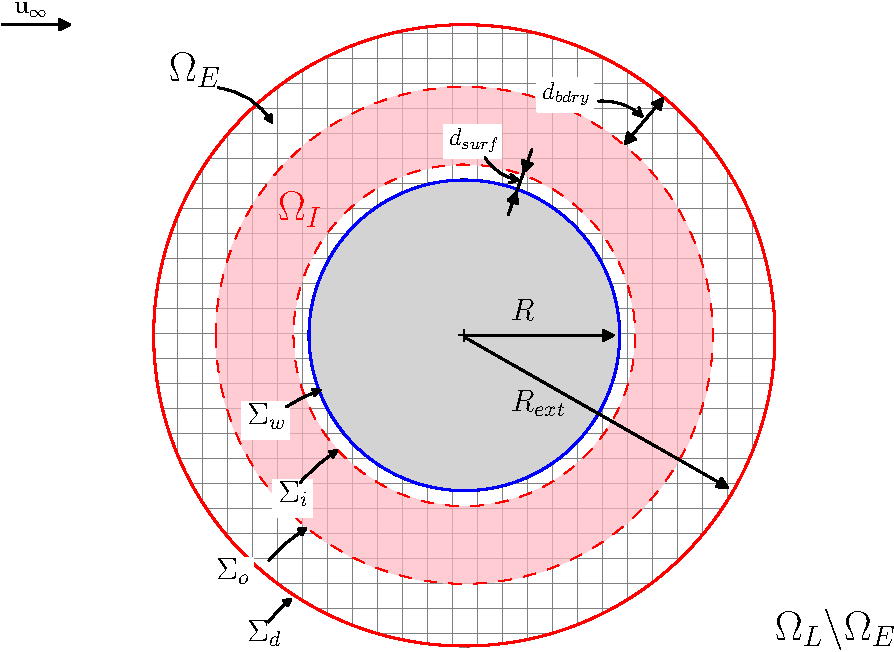
\includegraphics[width=0.6\linewidth]{./figures/validation/isc/hisc_dd-crop.pdf}
	\caption{(\textit{Not to Scale}) The domain decomposition for the Impulsively started cylinder. The parameters of the domain are tabulated in table \ref{tab:h_ISCParameters}.}
	\label{fig:hisc_dd}
	\end{figure}

	\ctable[
		caption = {Summary of the parameters of the hybrid simulation for the impulsively started cylinder test case at $Re=550$.},
		label   = {tab:h_ISCParameters},
		pos = !t,]{lcll}{}{\FL
		Parameters					& Value 				& Unit		& Description \ML
		$Re$  			       		& $550$ 				&-			& Reynolds number \\ 
		$\mathbf{u}_{\infty}$		& $[1,0]$ 				&\si{m.s^{-1}}& Freestream velocity\\		
		$R$			         		& $1$ 					&\si{m}		& Radius to Eulerian boundary $\Sigma_{wall}$\\		
 		$R_{ext}$ & 1.5 & \si{m} & Radius to Eulerian boundary $\Sigma_d$ \\
		$\nu$						& $\num{3.6e-3}$ 		&\si{kg.s^{-1}.m^{-1}}& Kinematic viscosity\\
		$\lambda$					& 1 & - & Overlap ratio\\
		$h$							& 0.008 & \si{m} & Nominal blob spacing\\		
		$h_{grid}$ 					& $0.008$ to $0.04$ & \si{m}	& FE cell diameter \\
		$ N_{\mathrm{cells}}$ 		& $32138$ 	& -						& Number of mesh cells\\						
		$N_{panels}$ & 100 & - & Number of panels\\
		$\Delta t_L$				& 0.005 & \si{s} & Lagrangian time step size\\
		$\Delta t_E$				& 0.001  & \si{s} & Eulerian time step size\\		
		$k_E$						& 5 & - & Number of Eulerian sub-steps\\			
		$ N_{\mathrm{t-steps}}$ 	& 40000 & -			& Number of time integration steps\\
		$t$							& 0 to 40 & - & Simulation time\\
		$d_{bdry}$					& $0.1\cdot{R}$ & \si{m} & Interpolation domain offset from boundary $\Sigma_d$\\
		$d_{surf}$					& $3\cdot{h}$ & \si{m} & Interpolation domain offset from boundary $\Sigma_{wall}$\LL}

Figure \ref{fig:hisc_dd} shows the domain decomposition of the hybrid simulation. The Lagrangian domain $\Omega_L$ resolves the full fluid domain, with an Eulerian domain $\Omega_E$ resolving the near-wall region of the cylinder. The interpolation domain $\Omega_I$ is defined by the inner boundary $\Sigma_i$ and the outer boundary $\Sigma_o$. The inner boundary $\Sigma_i$, is defined with an offset $d_{surf}=3\cdot{h}$ from the cylinder wall $\Sigma_{w}$ and the  outer boundary $\Sigma_{o}$ of the interpolation region $\Omega_{I}$ is defined with a larger offset $d_{bdry} = 0.1\cdot{R}$ from the boundary $\Sigma_d$. We observed in the previous test cases that the main error of the hybrid scheme is the artificial vorticity generated at the $\Sigma_d$ and therefore to minimize its influence, we have chosen a larger offset than used by Stock \cite{Stock2010a}.

%The initial boundary conditions of the Eulerian Dirichlet boundary $\Sigma_d$, is the velocity field induced by the vortex panels. At time progress, the vorticity is generated from the Eulerian boundary $\Sigma_{wall}$, transferring to the vortex blobs inside the interpolation region $\Omega_{int}$. 


\subsection{Results}

We investigated two aspects of the impulsively started cylinder problem. The first study focused on the impact of coupling parameters on the accuracy of the lift and the drag forces. The parameters of interest are the number of vortex panels $N_{panels}$, nominal blob spacing $h$, and time step size of the Lagrangian method $\Delta t_L$. The second study focused on the long run performance of the forces acting of the cylinder. Artificial perturbation was induced, as described in section \ref{subsec:eul_isc}, to induced vortex shedding at a smaller simulation time $t$.

Figure \ref{fig:hybrid_cylinder_contourComparison_tStarting} shows the vorticity contour at $t = [1,3,5,7]$. The plot compares the hybrid simulation (top halves) with the FE only simulation (bottom halves). The hybrid halves of the plot depicts the Eulerian sub-domain $\Omega_E$ in pink. After studying the figure, we observer that the vorticity contours of the hybrid simulation matches with the FE only simulation. The only difference between both simulation is the artificial vorticity emanating from the Dirichlet boundary $\Sigma_d$. However, we must note that the magnitude of the artificial vorticity is in the range $|\omega|\leqslant0.2$, and with the maximum vorticity in the domain $\max\{\omega\}=32$, we have that the strength of the artificial vorticity is less than $1\%$ of the maximum vorticity in the fluid. Therefore, we have ensured that the Lagrangian method and the Eulerian method has similar discretization at the region of overlap. In section \ref{sec:vvhm-love}, we determined that this is required to ensure an accurate coupling scheme.



	\begin{figure}[!t]
	\centering
	%\includegraphics[trim=0cm 2.5cm 0cm 2.5cm, clip, width=\linewidth]
	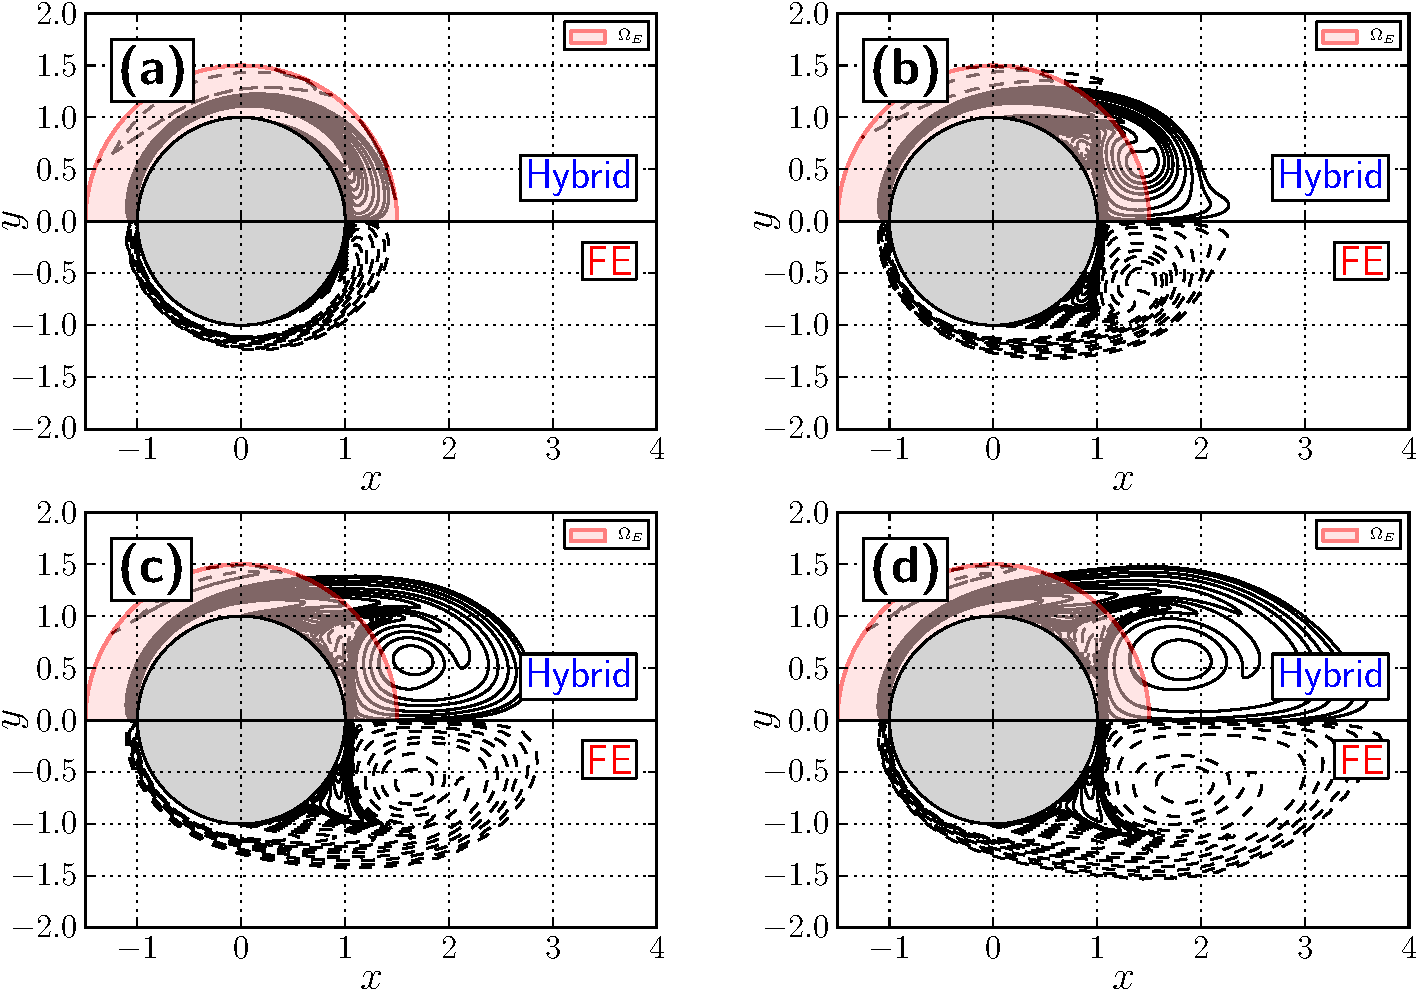
\includegraphics[width=\linewidth]{./figures/validation/isc/hybrid_cylinder_contourComparison_tStarting-crop.pdf}
	\caption{Comparison of the vorticity contours for \textbf{(a)} $t=1$, \textbf{(b)} $t=3$, \textbf{(c)} $t=5$ and \textbf{(d)} $t=7$ with contour levels $[-7,..., -3, -2, -1,$ $0.5, -0.2, -0.1, 0.1, 0.2, 0.5,$ $1, 2, 3,..., 7]$. The figures compares the hybrid simulation (top half) with FE only simulation (bottom half).}
	\label{fig:hybrid_cylinder_contourComparison_tStarting}
	\end{figure}

%	\begin{figure}[!p]
%     \centering
%     \begin{subfigure}[t]{0.49\textwidth}
%             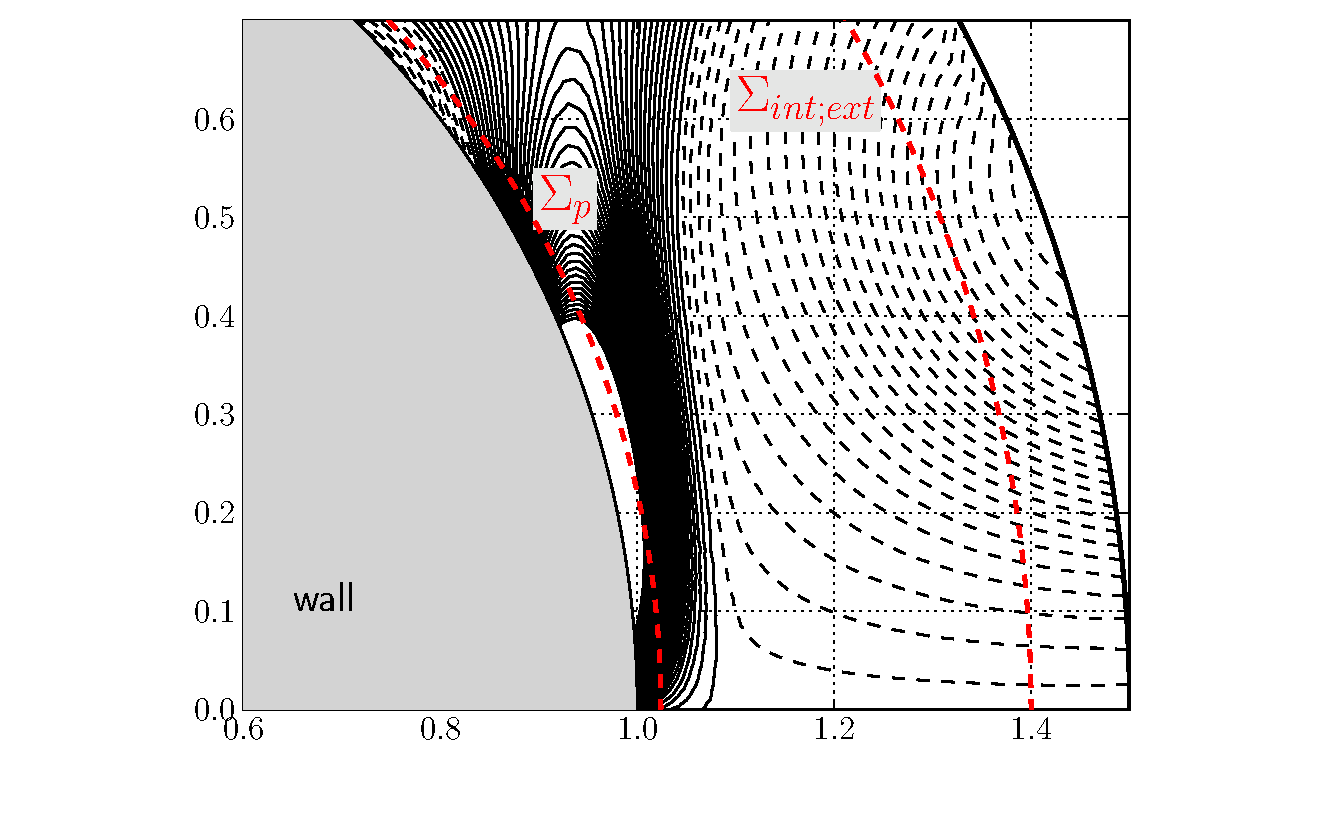
\includegraphics[width=\textwidth]{./figures/validation/isc/hisc_EulerianDomain_wall.pdf}
%             \caption{Wall region: Eulerian method}
%             \label{fig:hisc_EulerianDomain_wall}
%     \end{subfigure}%
%     ~ %add desired spacing between images, e. g. ~, \quad, \qquad etc.
%       %(or a blank line to force the subfigure onto a new line)
%     \begin{subfigure}[t]{0.49\textwidth}
%             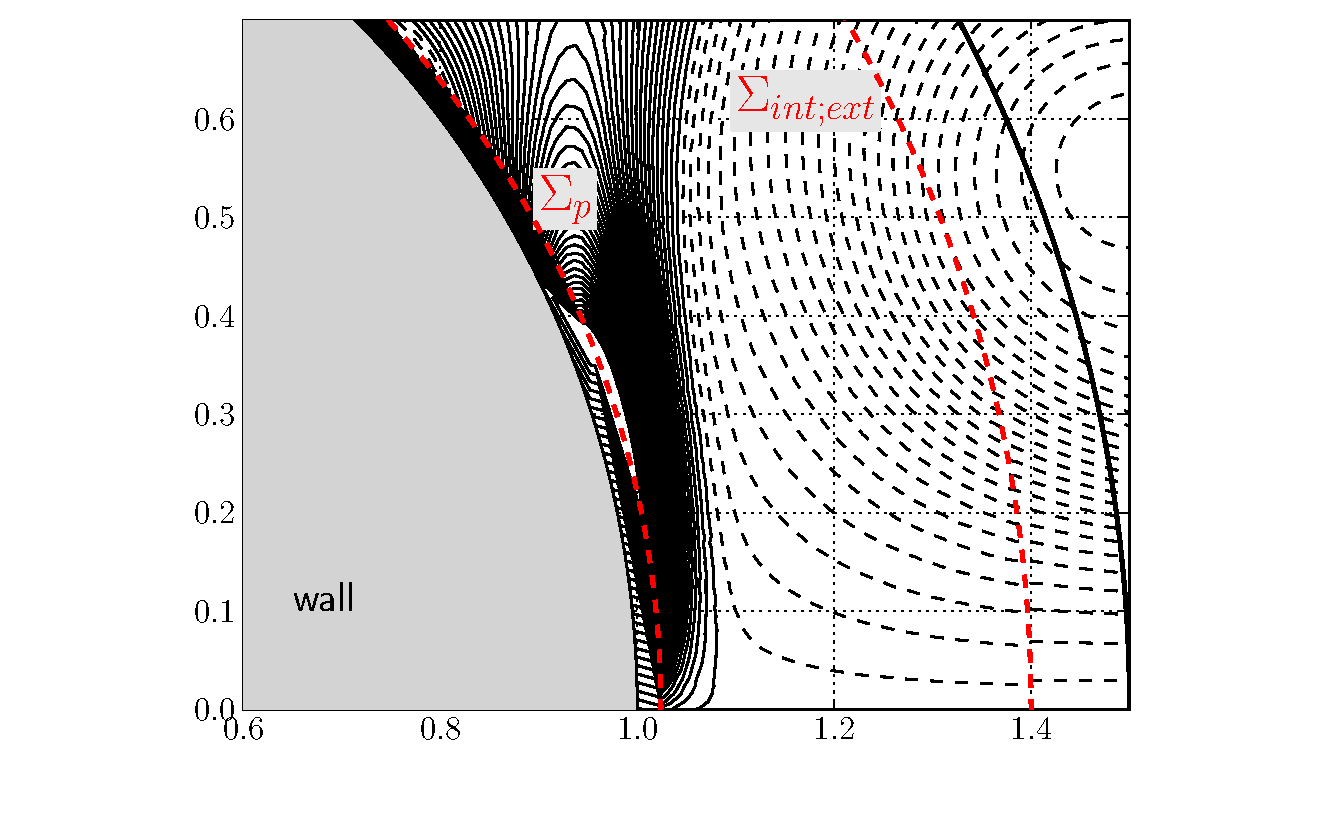
\includegraphics[width=\textwidth]{./figures/validation/isc/hisc_LagrangianDomain_wall.pdf}
%             \caption{Wall region: Lagrangian method}
%             \label{fig:hisc_LagrangianDomain_wall}
%     \end{subfigure}
%     
%     \begin{subfigure}[t]{0.49\textwidth}
%             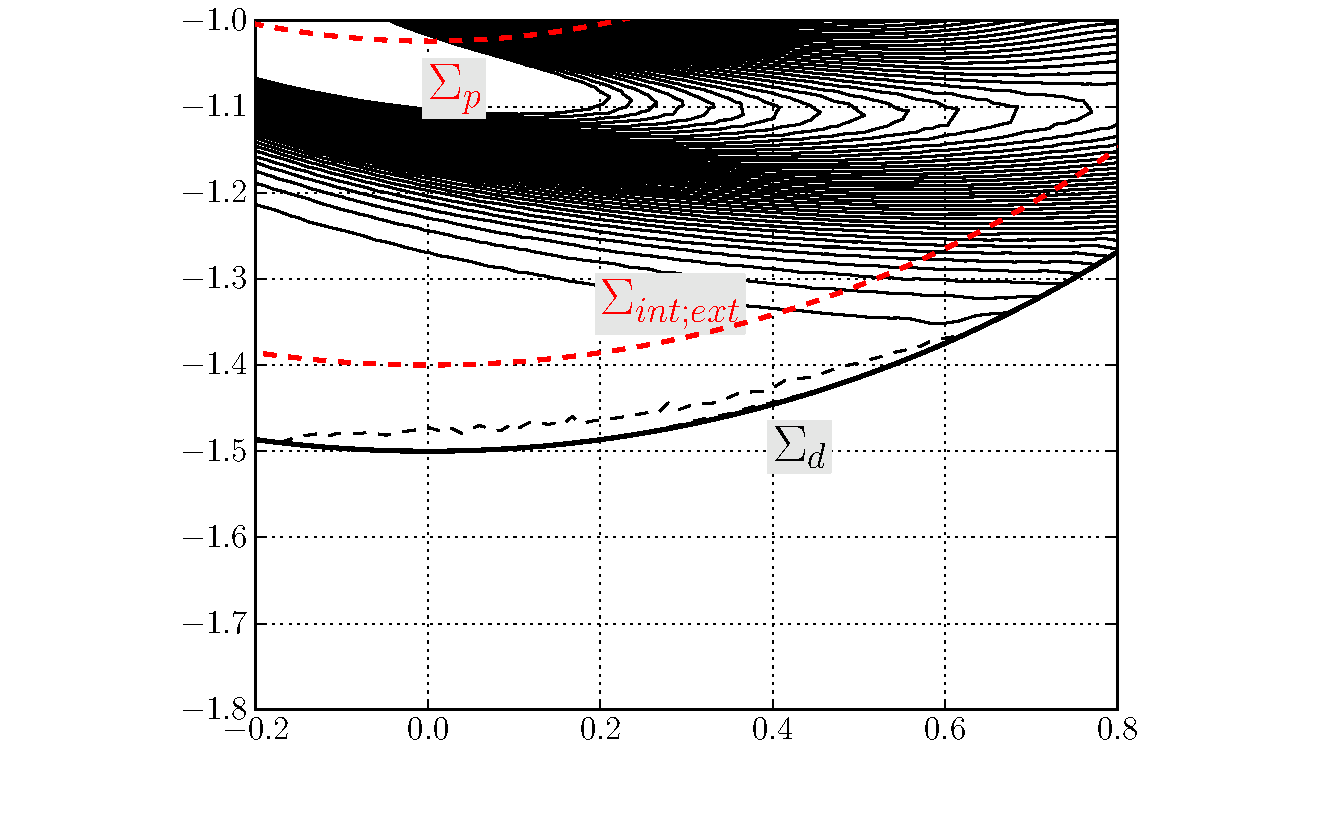
\includegraphics[width=\textwidth]{./figures/validation/isc/hisc_EulerianDomain_bdry.pdf}
%             \caption{Boundary region: Eulerian method}
%             \label{fig:hisc_EulerianDomain_bdry}
%     \end{subfigure}%
%     ~ %add desired spacing between images, e. g. ~, \quad, \qquad etc.
%       %(or a blank line to force the subfigure onto a new line)
%     \begin{subfigure}[t]{0.49\textwidth}
%             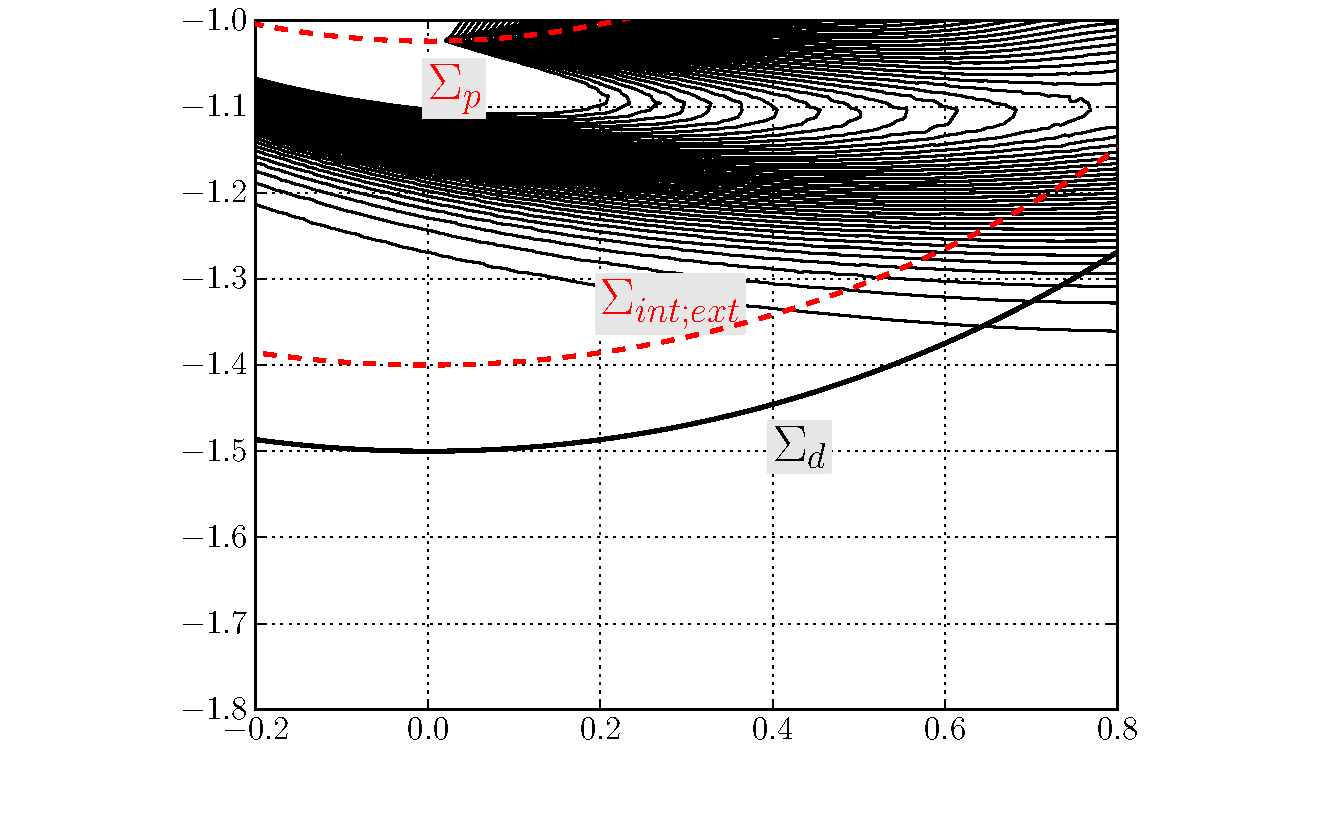
\includegraphics[width=\textwidth]{./figures/validation/isc/hisc_LagrangianDomain_bdry.pdf}
%             \caption{Boundary region: Lagrangian method}
%             \label{fig:hisc_LagrangianDomain_bdry}
%     \end{subfigure}     
%     \caption{Eulerian method and Lagrangian method resolutions}
%     \label{fig:hisc_EulerianVsLagrangian}
%	\end{figure}

	\begin{figure}[!p]
	\centering
	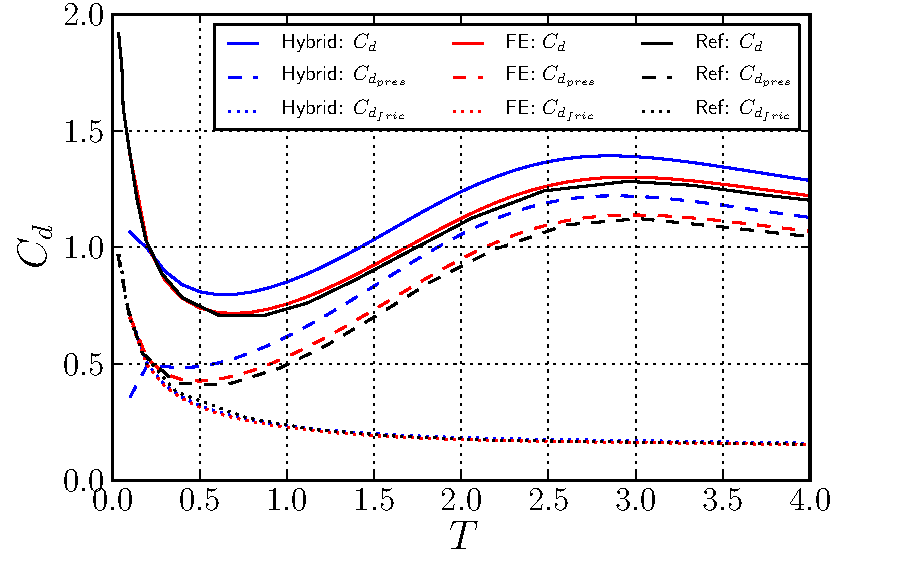
\includegraphics[width=0.6\linewidth]{./figures/validation/isc/hybrid_ISC_drag.pdf}
	\caption{ Evolution of the drag coefficient during the initial stages $t=0$ to $t=4$ with total drag coefficient $C_d$ (solid), pressure drag coefficient $C_{d_{pres}}$ (dashed) and friction drag coefficient $C_{d_{fric}}$ (dotted). The figure compares results of hybrid simulation ({\color{plotBlue}{\textbf{blue}}}), FE only simulation ({\color{plotRed}{\textbf{red}}}) and reference data (\textbf{black}) of Koumoutsakos and Leonard \cite{Koumoutsakos1995a}}
	\label{fig:hybrid_ISC_drag}
	\end{figure}

	\begin{figure}[!p]
     \centering
     \begin{subfigure}[t]{0.49\textwidth}
             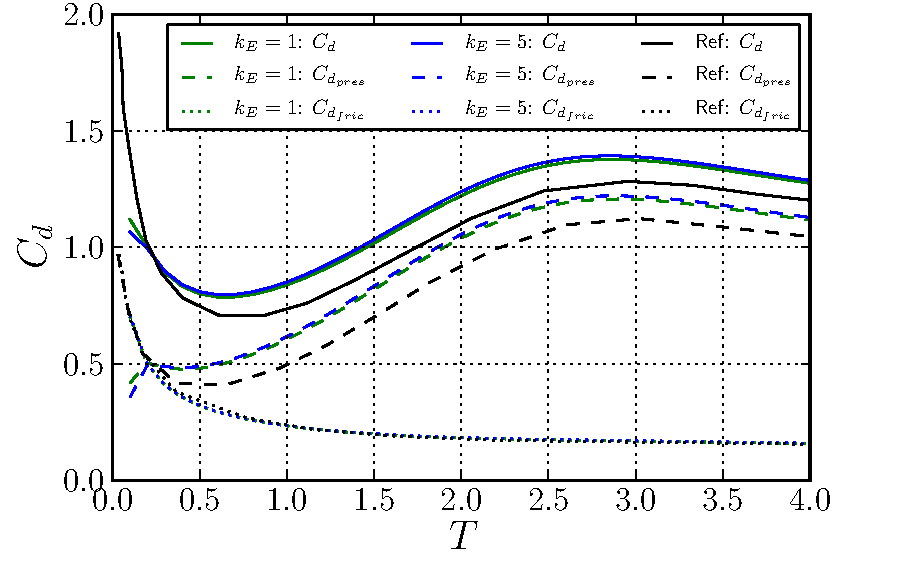
\includegraphics[width=\textwidth]{./figures/validation/isc/hybrid_ISC_drag_kComparison.pdf}
             \caption{Variation in Lagrangian time step size $\Delta t_L$: $k_E=1$ with $\Delta t_L = \Delta t_E$ and $k_E=5$ with $\Delta t_L = 5\cdot{\Delta t_E}$}
             \label{fig:hybrid_ISC_drag_kComparison}
     \end{subfigure}%
     ~ %add desired spacing between images, e. g. ~, \quad, \qquad etc.
       %(or a blank line to force the subfigure onto a new line)
     \begin{subfigure}[t]{0.49\textwidth}
             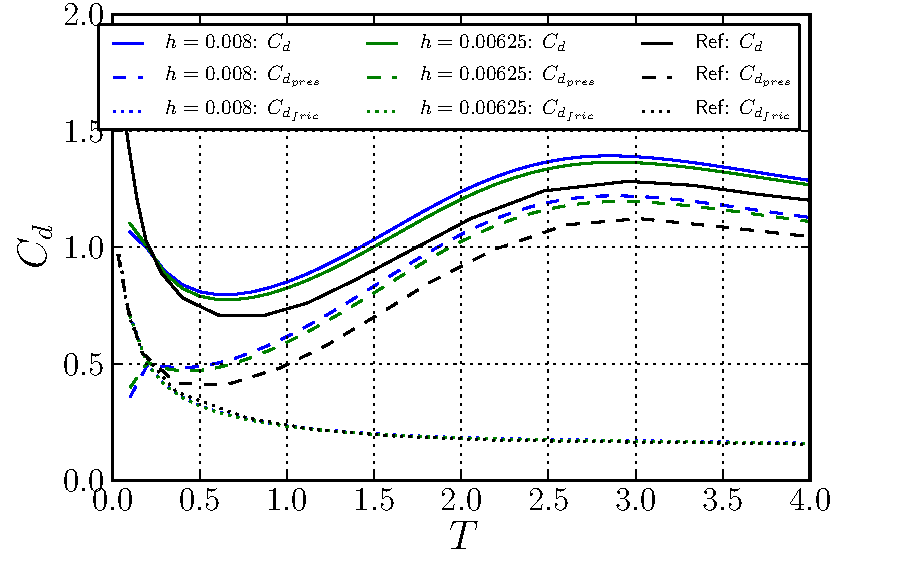
\includegraphics[width=\textwidth]{./figures/validation/isc/hybrid_ISC_drag_nBlobComparison.pdf}
             \caption{Variation in nominal blob spacing $h$: $h=0.008$ and $h=0.005$}
             \label{fig:hybrid_ISC_drag_nBlobComparison}
     \end{subfigure}
     
     \begin{subfigure}[b]{0.49\textwidth}
             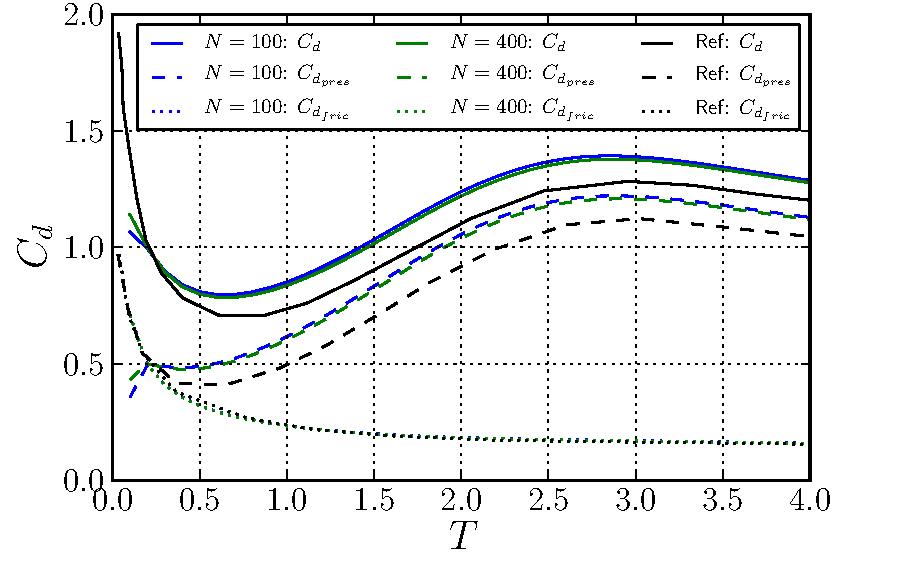
\includegraphics[width=\textwidth]{./figures/validation/isc/hybrid_ISC_drag_nPanelComparison.pdf}
             \caption{Variation in number of panels $N_{panels}$: $N=100$ and $N=400$}
             \label{fig:hybrid_ISC_drag_nPanelComparison}
	 \end{subfigure}
    
     \caption{Parameters sensitivity analysis on the drag evolution of the cylinder from $t=0$ to $t=4$, compared with literature data (\textbf{black}) obtained from Koumoutsakos and Leonard \cite{Koumoutsakos1995a}}
     \label{fig:hybrid_ISC_parameterSensitivity}
	\end{figure}
	
	
	\begin{figure}[!p]
	\centering
	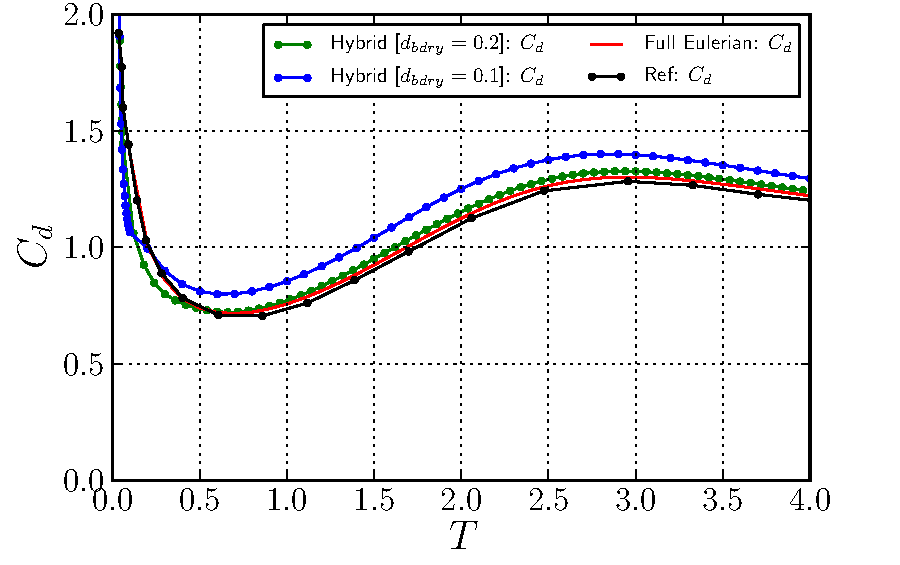
\includegraphics[width=0.6\linewidth]{./figures/validation/isc/hybrid_ISC_drag_comparison_dbdry2.pdf}
	\caption{Variation in $d_{bdry} = [0.1R, 0.2R]$. Compared with benchmark FE only simulation and literature, Koumoutsakos and Leonard \cite{Koumoutsakos1995a}}
	\label{fig:hybrid_ISC_parameterSensitivity_dbdry}
	\end{figure}	
	
	\begin{figure}[!p]
	\centering
	\includegraphics[width=0.6\linewidth]{./figures/validation/isc/hybrid_cylinder_LongRun_liftDrag.pdf}
	\caption{Evolution of the lift and drag coefficient from $t=0$ to $t=40$ with artificial perturbation \cite{Lecointe1984}. The figure compares hybrid ({\color{plotBlue}{\textbf{blue}}}), FE only ({\color{plotRed}{\textbf{red}}}), and the reference data (\textbf{black}) from Rosenfeld et al. \cite{MosheRosenFeldDochanKwak1991}.}
	\label{fig:hybrid_cylinder_LongRun_liftDrag}
	\end{figure}	



	\begin{figure}[!p]
	\centering
	\includegraphics[width=\linewidth]{./figures/validation/isc/hybrid_cylinder_LongRun_contourfComparison_compressed-crop.png}
	\caption{Plot of the vorticity field at $t=[10,20,30,40]$, comparing the hybrid simulation (left) with the FE only simulation (right).}
	\label{fig:hybrid_cylinder_LongRun_contourfComparison}
	\end{figure}
	

Figure \ref{fig:hybrid_ISC_drag} shows the evolution of the drag coefficient $C_d$, the friction drag $C_{d_{fric}}$, and the pressure drag $C_{d_{pres}}$. The results are compared with the FE only simulation and the reference data obtained from Koumoutsakos and Leonard \cite{Koumoutsakos1995a}. Observing the figure, we see that the hybrid simulation has a larger drag coefficient, due to the increased pressure drag $C_{d_{pres}}$. 

Varying the Lagrangian time step $\Delta t_L$, Figure \ref{fig:hybrid_ISC_drag_kComparison}, the nominal blob spacing $h$, Figure \ref{fig:hybrid_ISC_drag_nBlobComparison}, and the number of vortex panels, Figure \ref{fig:hybrid_ISC_drag_nPanelComparison}, we see that the accuracy of the simulation increases with increasing spatial and temporal resolution. The parameter sensitivity analysis showed that the simulation with $h=0.00625$ showed the largest improvement.

However, during the end of the present study it became apparent that other parameters of the hybrid method might also have an impact on the accuracy of the simulation. Figure \ref{fig:hybrid_ISC_parameterSensitivity_dbdry} shows the impact of increasing the $d_{bdry}$ of the interpolation domain. We see that with $d_{bdry}=0.2R$, there is much larger agreement with the benchmark results. However, determined the appropriate $d_{bdry}$ for a given flow condition becomes a challenging topic. As further increase of $d_{bdry}$ means that less of the Eulerian solution is transferred to the Lagrangian domain. This could also cause a detrimental effect as the now the simulation becomes less coupled. Therefore, we propose a future research on determining the appropriate $d_{bdry}$ such that the incorrect Eulerian solution at the boundary does not pose a concern to the coupling.



%Moreover, the drag coefficient is under-estimated at the first few time instances. To investigate further on the causes of this trends, we performed a parameter sensitivity analysis. 

%Figure \ref{fig:hybrid_ISC_parameterSensitivity} shows the impact of varying the resolution of the Lagrangian method w.r.t to the Eulerian method on the accuracy of the drag coefficient calculated. To reduce the artificial vorticity, we modified the Lagrangian time step size $\Delta t_L$, the nominal blob spacing $h$, and the number of vortex panels $N_{panels}$. 

%Figure \ref{fig:hybrid_ISC_drag_kComparison} investigates the effect of changing the Lagrangian time step size $\Delta t_L$ on the drag coefficient. The Lagrangian time step was varied with setting the number of Eulerian sub-steps $k_E$ to $k_E=1$ and $k_E=5$. With fixed Eulerian time step size $\Delta t_E=0.001$, the Lagrangian time step sizes were $\Delta t_L = 0.001$ and $\Delta t_L=0.005$, respectively. The figure shows that reducing the Lagrangian time-step size by a $5^{\mathrm{th}}$, only educes the error slightly. Therefore, varying the Lagrangian time-step size has only a minimal improvement.

%Figure \ref{fig:hybrid_ISC_drag_nBlobComparison} shows the effect of varying the nominal blob spacing $h$ from $h=0.008$ to $h=0.00625$. The figure shows that by a small increase he resolution of the blobs as a larger improvement on the drag coefficient, that varying the Lagrangian time step size. Therefore, to improve the coupling, it is more ideal to increase the spatial resolution of the Lagrangian method than the temporal resolution. 
%
%Figure \ref{fig:hybrid_ISC_drag_nPanelComparison} shows the effect of varying the number of vortex panels $N_{panels}$ from $N=100$ to $N=400$. Increasing the number of panels by $4$ times, has a smaller effect than the improvement of varying the resolution of the vortex blobs.


The second focus of the impulsively started cylinder is the long run evolution of the lift and the drag of the cylinder, from $t=0$ to $t=40$. We performed similar comparison as done in section \ref{subsec:eul_isc}. An artificial perturbation was induced according to Leocointe and Piquet \cite{Lecointe1984}. Figure \ref{fig:hybrid_cylinder_LongRun_liftDrag} compares the evolution of the lift coefficient $C_l$, and the drag coefficient $C_d$ of hybrid simulation, with the FE only simulation, and the reference data from Rosenfeld et al. \cite{MosheRosenFeldDochanKwak1991}. 

	\begin{figure}[!t]
     \centering
     \begin{subfigure}[t]{0.49\textwidth}
             \includegraphics[width=\textwidth]{./figures/validation/isc/hybrid_isc_firstDipole_hybrid_compressed-crop.png}
             \caption{Hybrid}
             \label{fig:hybrid_isc_firstDipole_hybrid_compressed-crop}
     \end{subfigure}%
     ~ %add desired spacing between images, e. g. ~, \quad, \qquad etc.
       %(or a blank line to force the subfigure onto a new line)
     \begin{subfigure}[t]{0.49\textwidth}
             \includegraphics[width=\textwidth]{./figures/validation/isc/hybrid_isc_firstDipole_FE_compressed-crop.png}
             \caption{FE only}
             \label{fig:hybrid_isc_firstDipole_FE_compressed-crop}
     \end{subfigure}
     \caption{Plot of the first shed vortex at $t=40$, comparing (\textbf{a}) the hybrid simulation, and (\textbf{b}) the FE only simulation.}
     \label{fig:hybrid_isc_firstDipole}
	\end{figure}

Investigating the evolution of drag shows that the hybrid simulation has higher drag. After $t=5$, there is slight mismatch in the oscillation of the drag. However observing the amplitude fluctuation, we see that the simulation tend to fluctuate around $C_d=1.4$. Observing the evolution of lift shows that the hybrid simulation has a larger initial amplitude. Furthermore, there exist a negative phase shift in the amplitude. However, at time progress, $t>20$, we see that the frequency and the amplitude of the oscillation is similar to the reference data. A through investigation of the oscillation requires a longer simulation where the amplitude of the oscillation would become fixed. However, due to the lack of computational resources, a longer simulation than $t=40$ with the current simulation parameters was not feasible.

Figure \ref{fig:hybrid_cylinder_LongRun_contourfComparison} compares the vorticity field of the hybrid simulation (left), and the FE only simulation (right) at time instances $t=[10,20,30,40]$. We see that the initial vorticity distribution are in good agreement. As time progress, the simulations deviate away from each other and is simply due to the difference in the spatial discretization.

The difference in the spatial discretization becomes apparent in Figure \ref{fig:hybrid_isc_firstDipole}, The figure shows the state of the first shed vortex at $t=40$, for the hybrid simulation and the FE only simulation. For an efficient FE only simulation, we had to under-resolve the mesh, away from the cylinder. However, with the auto-adaptive nature of the Lagrangian method, the hybrid simulation has a well defined first vortex core. Furthermore, we see that the dipole sustains is strength, unlike the FE only simulation with is more diffusive, when under-resolved.


\subsection{Discussion of Results}	

In conclusion, the results of the impulsively started cylinder test cases showed that:
\begin{itemize}
\item When the hybrid method is under-resolved, the cylinder experience a higher drag.
\item Increasing the boundary offset $d_{bdry}$ from $0.1R$ to $0.2R$ improved the simulation results. However, an increased offset also means less coupled results as more Eulerian solution is ignored. This can have detrimental effect for high Reynolds number flows.
\end{itemize}

As the present study was limited with computational resource and time, a detailed investigation of the $d_{bdry}$ could not be performed. A research in future in this regard could help us determine the ideal $d_{bdry}$ for a given flow condition.

Due to the limited computation resources and time, the long run simulation was performed with less regard on the accuracy. However, the results showed that even with less resolved method, the hybrid method is capable of observing similar oscillations as the well-resolved FE only simulation. In addition to this, when observing the starting vortex at $t=40$, it became apparent that the hybrid method provides a well-resolved solution even at $D=13$. This highlights the advantage of the auto-adaptive nature of the hybrid method and the ease of resolves an unsteady vorticity field.

If the hybrid method can provide additional accuracy without sacrificing the efficiency, for example with $d_{bdry}=0.2R$, the hybrid method has the potential to substantially outperform the convectional grid methods for unsteady flow problems of a VAWT.


%We were also able to observe the auto-adaptive nature of our hybrid scheme. The first vortex shed from the cylinder, was still well-resolved at $t=40$ in the hybrid scheme, whereas the FE only simulation failed to sustain the structure and the strength of the vortex. 

%In conclusion, we 
\section{Stalled Elliptic Airfoil at $Re=5000$}
\label{sec:vvhm-ea}

The purpose of investigating the stalled elliptical airfoil at $Re=5000$ is to demonstrate the feasibility of using the hybrid method to simulate a complex problem, such as a flow around a thin stalled airfoil. The FE only simulation is as a benchmark for the current study.
\subsection{Problem Definition}

The study of the stalled elliptical airfoil at $RE=5000$, is performed similarly to the study of the impulsively started cylinder at $Re=550$, see section \ref{sec:vvhm-isc}. The main difference now is the mesh geometry (now representing a thin stalled airfoil), and a higher Reynolds number.

Figure \ref{fig:hellipticAirfoil_dd-crop} depicts the configuration of the hybrid simulation. We studied the flow around a thin airfoil with thickness to chord ratio $t/c$ of $12\%$, having a with a chord length $L=1$, and a maximum thickness $W=0.12$. As we have a elliptical airfoil, the maximum thickness is located at $0.5L$. Furthermore, the airfoil is pitched to $20^{\circ}$ about center of rotation $0.25L$, to create a stalled flow. The parameters of the simulation are summarized in table \ref{tab:h_ea_Parameters}. 


	\begin{figure}[!t]
	\centering
	%\includegraphics[trim=0cm 2.5cm 0cm 2.5cm, clip, width=\linewidth]
	\includegraphics[width=0.6\linewidth]{./figures/validation/ellipse/hellipticAirfoil_dd-crop.pdf}
	\caption{(\textit{Not to scale}) The domain decomposition for the stalled elliptical airfoil. The parameters of the domain are tabulated in table \ref{tab:h_ea_Parameters}.}
	\label{fig:hellipticAirfoil_dd-crop}
	\end{figure}

	\ctable[
		caption = {Summary of the parameters of the hybrid simulation for the stalled elliptical airfoil test case.},
		label   = {tab:h_ea_Parameters},
		pos = !t,]{lcll}{}{\FL
		Parameters					& Value 				& Unit		& Description \ML
		$Re$  			       		& $5000$ 				&-			& Reynolds number \\ 
		$\mathbf{u}_{\infty}$		& $[1,0]$ 				&\si{m.s^{-1}}& Freestream velocity\\		
		$L$			         		& $1$ 					&\si{m}		& Chord length\\		
		$W$			         		& $0.12$ 				&\si{m}		& Maximum thickness\\		
 		$\nu$						& $\num{2e-4}$ 		&\si{kg.s^{-1}.m^{-1}}& Kinematic viscosity\\
		$\lambda$					& 1 & - & Overlap ratio\\
		$h$							& \num{1.67e-3} & \si{m} & Nominal blob spacing\\		
		$h_{grid}$ 					& $0.0014$ to $0.008$ & \si{m}	& FE cell diameter \\
		$ N_{\mathrm{cells}}$ 		& $118196$ 	& -						& Number of mesh cells\\						
		$N_{panels}$ & 400 & - & Number of panels\\
		$\Delta t_L$				& \num{1e-4} & \si{s} & Lagrangian time step size\\
		$\Delta t_E$				& \num{1e-3}  & \si{s} & Eulerian time step size\\		
		$k_E$						& 10 & - & Number of Eulerian sub-steps\\			
		$ N_{\mathrm{t-steps}}$ 	& 10000 & -			& Number of time integration steps\\
		$t$							& 0 to 10 & - & Simulation time\\
		$d_{bdry}$					& $0.1\cdot{L}$ & \si{m} & Interpolation domain offset from boundary $\Sigma_d$\\
		$d_{surf}$					& $3\cdot{h}$ & \si{m} & Interpolation domain offset from boundary $\Sigma_{wall}$\LL}

\subsection{Results}

The results shows the hybrid method is capable of simulating the flow past a lifting body. Figure \ref{fig:hybrid_ellipseForce} shows the evolution of the lift and the drag coefficient. We see that the lift and the drag coefficient are in good agreement upto $t=2$. However, as time progress we see the results of the simulation deviate from each other. A possible explanation is the higher Reynolds number. When we deal with higher Reynolds number, we see that coupling procedure is more sensitive.

% The lift and the drag forces determined by the hybrid method matches upto $t=2$. The oscillation of the lift after $t=3$ is fundamentally different, which peaks occuring at different time instances. Similarly, the peak drag occurs at different time instances, however we can see that the maximum and minimum drag coefficient during is similar. 


% Figure \ref{fig:hybrid_ellipse_HybridvsFE_contourDeviation} compares the vorticity plot of hybrid and the FE only simulation at time instances $t=[1,2,3,4]$. We see that the results of the simulation are in good agreement for the initial time-steps. However, as we a Reynolds number $Re=5000$, we obser
%
%It is apparent that from $t=3$, the structure of the shed vorticity is different. For higher Reynolds number flows, the error in the coupling, seemed to have a greater impact on the evolution of the vorticity field. 
%
%	\begin{figure}[!t]
%	\centering
%	\includegraphics[width=\linewidth]{./figures/validation/ellipse/hybrid_ellipse_HybridvsFE_contourDeviation_compressed-crop.png}
%	\caption{hybrid ellipse HybridvsFE contourDeviation}
%	\label{fig:hybrid_ellipse_HybridvsFE_contourDeviation}
%	\end{figure}

%To further investigate the effect of the artificial vorticity, we investigated the evolution of the lift and the drag forces, depicted in Figure \ref{fig:hybrid_ellipseForce}. The lift and the drag forces determined by the hybrid method matches upto $t=2$. The oscillation of the lift after $t=3$ is fundamentally different, which peaks occuring at different time instances. Similarly, the peak drag occurs at different time instances, however we can see that the maximum and minimum drag coefficient during is similar. 

Figure \ref{fig:hybrid_ellipse_Hybrid_contours} shows the plot of vorticity field at $t=[1,2,3,...,10]$. We see that thanks to adaptive nature of the scheme, the shed vortices are well-defined. Furthermore, in the near-wall region, the Eulerian region is able to capture the complex stalled structure of the airfoil.
	
	\begin{figure}[!p]
     \centering
     \begin{subfigure}[t]{0.49\textwidth}
             \includegraphics[width=\textwidth]{./figures/validation/ellipse/hybrid_ellipseForce_CL.pdf}
             \caption{Hybrid}
             \label{fig:hybrid_ellipseForce_CL}
     \end{subfigure}%
     ~ %add desired spacing between images, e. g. ~, \quad, \qquad etc.
       %(or a blank line to force the subfigure onto a new line)
     \begin{subfigure}[t]{0.49\textwidth}
             \includegraphics[width=\textwidth]{./figures/validation/ellipse/hybrid_ellipseForce_CD.pdf}
             \caption{FE only}
             \label{fig:hybrid_ellipseForce_CD}
     \end{subfigure}
     \caption{Forces}
     \label{fig:hybrid_ellipseForce}
	\end{figure}	

	\begin{figure}[!p]
	\centering
	\includegraphics[width=\linewidth]{./figures/validation/ellipse/hybrid_ellipse_Hybrid_contours_compressed-crop.png}
	\caption{Plot of the vorticity contours at $t=[1,2,3,4,5,6,7,8,9,10]$.}
	\label{fig:hybrid_ellipse_Hybrid_contours}
	\end{figure}
	
\subsection{Discussion of results}	

The results of the stalled elliptical airfoil at $Re=5000$ showed that:
\begin{itemize}
\item The hybrid method is able to simulate the unsteady flow separation.
\item A higher Reynolds number flow problem is still a challenge and accuracy has only achieved upto $t=2$.
\end{itemize}

The simulation showed that the present hybrid method is capable of simulating the flow past an airfoil that undergoes a unsteady flow separation. This is a key aspect of the VAWT simulation and the through this test case we have shown the capability of simulation the flow of a VAWT blades.

However, for the Reynolds number regimes of VAWT, turbulence models such as URANS and LES are fundamental requirement for efficient and accurate computation of the flow. Furthermore, we also require the implementation of the moving body to with requires an Arbitrary Lagrangian-Eulerian formulation for the Eulerian domain. A research in this regards in an essential towards the development of the hybrid method for VAWT.

%However, due the large number of parameters that have an influence on the accuracy of the simulation, such as the number of panels, nominal particle spacing, overlap ration, particle core size, the diffusion scheme.


	
\section{Multi-body problem}
\label{sec:vvhm-mb}

The hybrid method has the feasibility of simulating the flow about multiple decomposed Eulerian domains. To demonstrate this feasibility, we simulated the flow around two impulsively started cylinders with segregated Eulerian domains. 

\subsection{Problem Definition}

The parameters of the simulation are shown in table \ref{tab:h_ISCParameters}. The two cylinder configuration is represented by two Eulerian sub-domains, $\Omega_{E_{A}}$ and $\Omega_{E_B}$, belonging to cylinder $A$ and cylinder $B$ respectively. The configuration of the two cylinder is depicted in Figure \ref{fig:hmisc_dd-crop}. The locations of the cylinder $A$ and $B$ are at $(x_A,y_A) = (-R_{ext},0)$ and $(x_B,y_B) = (R_{ext},R)$, respectively. These positions ensure that the Eulerian sub-domains do not overlap, and the Lagrangian method is used to communicate between theses sub-domains.

	\begin{figure}[!h]
	\centering
	\includegraphics[width=0.6\linewidth]{./figures/validation/multipleCylinder/hmisc_dd-crop.pdf}
	\caption{(\textit{Not to Scale}) The hybrid domain decomposition configuration of two impulsively started cylinder test case. }
	\label{fig:hmisc_dd-crop}
	\end{figure}

\subsection{Results}

The simulation of multi-body problem was ran upto $t=22$, reaching the limit of the computational resource. Figure \ref{fig:hybrid_multipleCylinder_contours_compressed-crop} shows the plot of the vorticity at various time instances, at $t=[1,4,7,10,13,16,19,22]$. The plot shows the transfer of vorticity from cylinder $A$ to cylinder $B$ with the help of the Lagrangian method. The Lagrangian method serves as the global communication tool for transferring the information between various Eulerian sub-domains. 

	\begin{figure}[!p]
	\centering
	\includegraphics[width=\linewidth]{./figures/validation/multipleCylinder/hybrid_multipleCylinder_contours_compressed-crop.png}
	\caption{Plot of the vorticity contours at $t=[1,4,7,10,13,16,19,22]$ at $Re=550$.}
	\label{fig:hybrid_multipleCylinder_contours_compressed-crop}
	\end{figure}

\subsection{Discussion of results}

The simulation shows the feasibility of simulating a multi-body problem. The advantage of the hybrid method for such problems is that, in future when the moving body problem is implemented, the two bodies can move independently. In a convectional grid method, where the two methods have to share a single Eulerian domain, the determination of efficient mesh becomes a non-trival aspect.

In conclusion, we see that the hybrid method is capable of simulating a multi-body VAWT problem with greater ease than the convectional grid based method.

% two body can be moved independent to each other. In future, when a moving body problem is implemented, the two Eulerian domains can 

%Therefore, by extending the current hybrid method implementation to take in account of the moving body, it should be feasible to simulate a VAWT simulation.

%\section{Discussion of conclusions}





